% !TEX encoding = UTF-8 Unicode
% !TEX TS-program = pdflatex
\newif\ifprint % to compile the print version or the digital one
\printtrue     % to compile the print version
\printfalse    % to compile the digital version  (default) - comment this line to compile the print version
% toptesti document class
\documentclass[%
    a4paper, % not needed, by default it is a4paper, or also b5paper can be used
    corpo=12pt, % dimension of basic font
    % oneside is generally the way to go
    oneside, % two side optimizes for two-face printing, having chapters open on the right (aka odd numbers), if you don't want blank pages put oneside here
    stile=standard,
    %evenboxes, % not needed, to put supervisors and candidate at the same level
    tipotesi=magistrale,
    numerazioneromana, % roman numbering for appendixes and preambles, up to Table of Contents
    openright, % to force opening on the right for double-sided printing
    cucitura=0mm, % for printing, 7mm should be enough
    %dvipsnames, % for compatibility with xcolor, it does not work
]{toptesi}

%%%%%%%%%%%%%%%%%%%%%%%%%%%%%%%%%%%%%%%%%%%%%%%%%%%%
\usepackage[english]{babel}
\usepackage[utf8]{inputenc}
\usepackage[T1]{fontenc}
\usepackage{lmodern}

\usepackage{hyperref} % must be loaded before glossaries-extra

% bibliography
\usepackage[hyperref=true,backref=true,backend=biber,maxbibnames=9,maxcitenames=2,style=numeric,citestyle=numeric,sorting=none]{biblatex} % hyperref uses links, backref goes back to citations, uses biber as backend, with 9 names at most in bibliography and 2 in citations, citing using numbers, and sorting in citation order
% sorting can be also ydnt for year descending, name, title or ynt for ascending year

\usepackage{adjustbox} % to resize boxes by keeping the same aspect ratio
\usepackage{algorithm} % algorithm environment
\usepackage{algpseudocode} % improved pseudo-code
\usepackage{amsfonts}               %  AMS mathematical fonts
\usepackage{amsmath}
\usepackage{amssymb}                %  AMS mathematical symbols
\usepackage{bm}                     %  black/bold mathematical symbols
\usepackage{booktabs}               %  better tables
\usepackage[labelfont=bf]{caption} % font=footnotesize % to have reduced caption font size
\usepackage{csquotes}
\usepackage{enumitem} %left align the bulleted points
\usepackage{geometry}
%\usepackage{glossaries} % to use acronyms and glossary, it has also glossaries-extra as extension, but commands are different
\usepackage[%
    toc, % puts the link in the ToC
    %record = on, % to avoid use bib2gls
    abbreviations, % to load abbreviations / acronyms
    symbols, % to load symbols  A.P.
    acronyms, % to load acronyms A.P.
    automake, % to make the glossaries automatically A.P.
    %nonumberlist, % to avoid printing the numbers of the references in the acronyms page
]{glossaries-extra}
\usepackage{graphicx}               %  post-script images
%\usepackage{iwona} % extra fonts, substitute standard ones
\usepackage{listings} % to insert formatted code
\usepackage{lipsum} % for lorem ipsum text, not needed in the real work
\usepackage{makecell} % to change dimensions of cells, for math cases
\usepackage{mathtools} % for additional commands
\usepackage{mfirstuc} % to have capitalization capabilities
\usepackage[final]{microtype}      % microtypography, final lets latex use it also in bibliography
\usepackage{multirow} % to allow for cells covering more than 1 row in tables
\usepackage{nicefrac}       % compact symbols for 1/2, etc.
%\usepackage[lofdepth,lotdepth]{subfig}
\usepackage{ragged2e} % for justifying text
\usepackage{siunitx} % support for SI units of measurement and number typesetting
%\usepackage{subfig} A.P. i used subcaption instead
\usepackage{svg} % for svg support, works only if inkscape is installed, default for Overleaf v2
%\usepackage{subfigure}              %  subfigure compatibility, can be removed if subfig
\usepackage{tabularx} % equal-width columns in tables
\usepackage{textcomp} % extra fonts and symbols
\usepackage{url}            % simple URL typesetting
\usepackage{verbatim} % for extended verbatim support
\usepackage{xcolor} % to define colors and use standard CSS names add dvipsnames as option, but it clashes with xcolor loaded in toptesi, pay attention that if it goes in conflict with tikz/beamer, simply use \documentclass[usenames,dvipsnames]{beamer}, along with other custom options when defining the document class

% here ARIEL PRIARONE ADDED:
\usepackage{pgf}
\usepackage{pgfplots}
\DeclareUnicodeCharacter{2212}{−}
\usepgfplotslibrary{groupplots,dateplot}
\usetikzlibrary{patterns,shapes.arrows}
\pgfplotsset{compat=newest}
\usepackage{caption}
\usepackage{subcaption}
\usepackage{layouts}
\usepackage{dsfont}
\usepackage{xfrac}
%\usepackage{fontspec}
\def \thesisAxisWidth {\linewidth}
\def \thesisFigFontsize {8}

% configuration for glossaries
% convert and load converted glossaries in .tex ,format from .bib
\setabbreviationstyle{long-short-desc} % style before loading resources
% this command sets the style to title for long names of acronyms only in the glossary description, leading to capitalized first-letter for all words
% \glssetcategoryattribute{\glsxtrabbrvtype}{glossname}{capitalisewords} % doesn't work
% resources to load if using a bib file with bib2gls
%\GlsXtrLoadResources[%
% src={glossaries}, % name of the file without extension
% selection=all, % select all the entries
%]
% not needed
%\newglossary*{abbreviation}{Acronyms} % to change the name of this glossary for acronyms

%\renewcommand{\glsclearpage}{\paginavuota} % to allow glossaries to clear pages, done manually is better


% setup for hyperref
\hypersetup{%
    pdfpagemode={UseOutlines},
    bookmarksopen,
    pdfstartview={FitH},
    colorlinks,
    linkcolor={black}, % it is suggested to keep them black, since when printing it it costs per page, and if they have color it's twice the price per page
    citecolor={black},
    urlcolor={black}
  }
%

% setup for svg
\svgsetup{%
    inkscapeformat=pdf, % to force usage of PDF
    inkscapelatex=false, % to disable latex rendering of text, produces errors
}

% setup for siunitx, it does not work in the summary
\sisetup{%
    detect-all, % to use the same font as for writing when using \num
    mode=text, % to allow it to work also in math mode
    group-separator = {,}, % separator for number grouping
    group-minimum-digits = 3, % minimum number of digits a number must have to be grouped in 3-digit groups
}

% listings colours
\definecolor{rulecolor}{rgb}{0,0,0}
\definecolor{commentcolor}{rgb}{0,0.6,0}
\definecolor{linenumbercolor}{rgb}{0.5,0.5,0.5}
\definecolor{keywordcolor}{rgb}{0,0,0.95}
\definecolor{backcolor}{rgb}{1,1,1}%{0.95,0.95,0.92}
\definecolor{stringcolor}{rgb}{0.58,0,0.82}

% setup for lstlisting
\lstset{ %
	backgroundcolor=\color{backcolor},   % choose the background color; you must add \usepackage{color} or \usepackage{xcolor}; should come as last argument
	basicstyle=\footnotesize,        % the size of the fonts that are used for the code
	breakatwhitespace=false,         % sets if automatic breaks should only happen at whitespace
	breaklines=true,                 % sets automatic line breaking
	captionpos=t,                    % sets the caption-position to bottom
	commentstyle=\color{commentcolor},    % comment style
	extendedchars=true,              % lets you use non-ASCII characters; for 8-bits encodings only, does not work with UTF-8
	frame=single,	                   % adds a frame around the code
	keepspaces=true,                 % keeps spaces in text, useful for keeping indentation of code (possibly needs columns=flexible)
	keywordstyle=\color{keywordcolor},       % keyword style
	%language=VHDL,                 % the language of the code
	numbers=left,                    % where to put the line-numbers; possible values are (none, left, right)
	numbersep=5pt,                   % how far the line-numbers are from the code
	numberstyle=\tiny\color{linenumbercolor}, % the style that is used for the line-numbers
	rulecolor=\color{rulecolor},         % if not set, the frame-color may be changed on line-breaks within not-black text (e.g. comments (green here))
	showspaces=false,                % show spaces everywhere adding particular underscores; it overrides 'showstringspaces'
	showstringspaces=false,          % underline spaces within strings only
	showtabs=false,                  % show tabs within strings adding particular underscores
	stepnumber=1,                    % the step between two line-numbers. If it's 1, each line will be numbered
	stringstyle=\color{stringcolor},     % string literal style
	tabsize=4,	                   % sets default tabsize to 2 spaces
	title=\lstname,                   % show the filename of files included with \lstinputlisting; also try caption instead of title
	inputencoding=utf8,
	literate=
	{á}{{\'a}}1 {é}{{\'e}}1 {í}{{\'i}}1 {ó}{{\'o}}1 {ú}{{\'u}}1
	{Á}{{\'A}}1 {É}{{\'E}}1 {Í}{{\'I}}1 {Ó}{{\'O}}1 {Ú}{{\'U}}1
	{à}{{\`a}}1 {è}{{\`e}}1 {ì}{{\`i}}1 {ò}{{\`o}}1 {ù}{{\`u}}1
	{À}{{\`A}}1 {È}{{\'E}}1 {Ì}{{\`I}}1 {Ò}{{\`O}}1 {Ù}{{\`U}}1
	{ä}{{\"a}}1 {ë}{{\"e}}1 {ï}{{\"i}}1 {ö}{{\"o}}1 {ü}{{\"u}}1
	{Ä}{{\"A}}1 {Ë}{{\"E}}1 {Ï}{{\"I}}1 {Ö}{{\"O}}1 {Ü}{{\"U}}1
	{â}{{\^a}}1 {ê}{{\^e}}1 {î}{{\^i}}1 {ô}{{\^o}}1 {û}{{\^u}}1
	{Â}{{\^A}}1 {Ê}{{\^E}}1 {Î}{{\^I}}1 {Ô}{{\^O}}1 {Û}{{\^U}}1
	{œ}{{\oe}}1 {Œ}{{\OE}}1 {æ}{{\ae}}1 {Æ}{{\AE}}1 {ß}{{\ss}}1
	{ű}{{\H{u}}}1 {Ű}{{\H{U}}}1 {ő}{{\H{o}}}1 {Ő}{{\H{O}}}1
	{ç}{{\c c}}1 {Ç}{{\c C}}1 {ø}{{\o}}1 {å}{{\r a}}1 {Å}{{\r A}}1
	{€}{{\euro}}1 {£}{{\pounds}}1 {«}{{\guillemotleft}}1
	{»}{{\guillemotright}}1 {ñ}{{\~n}}1 {Ñ}{{\~N}}1 {¿}{{?`}}1
}


% biblatex setup
% generally 9000 is ok, if higher than 10000 it's bad
% If you want to break on URL numbers
\setcounter{biburlnumpenalty}{9000}
% If you want to break on URL lower case letters
\setcounter{biburllcpenalty}{9000}
% If you want to break on URL UPPER CASE letters
\setcounter{biburlucpenalty}{9000}


% how to change Contents to Table of Contents
\addto\captionsenglish{% Replace "english" with the language you use
  \renewcommand{\contentsname}%
    {Table of Contents}%
}

% to change the name of Abbreviations to Acronyms
% not needed if use use entry types and define those
% \renewcommand{\abbreviationsname}{Acronyms}

% to allow line comments in algorithms
\algnewcommand{\LineComment}[1]{\State \(\triangleright\) #1}

% to declare abs and norm
\DeclarePairedDelimiter\abs{\lvert}{\rvert}%
\DeclarePairedDelimiter\norm{\lVert}{\rVert}%

% Swap the definition of \abs* and \norm*, so that \abs
% and \norm resizes the size of the brackets, and the 
% starred version does not.
\makeatletter
\let\oldabs\abs
\def\abs{\@ifstar{\oldabs}{\oldabs*}}
%
\let\oldnorm\norm
\def\norm{\@ifstar{\oldnorm}{\oldnorm*}}
\makeatother

%% *** ARIEL PRIARONE ***
\let\dummy\autoref % This redefine autoref as dummy
\def\autoref#1{\textbf{\dummy{#1}}} % this is like \autoref but in bold
\newcommand{\algorithmautorefname}{algorithm} % to make autoref work with algorithms
\addto\extrasenglish{\def\figureautorefname{figure}}%
\addto\extrasenglish{\def\chapterautorefname{chapter}}%
\addto\extrasenglish{\def\sectionautorefname{section}}%
\addto\extrasenglish{\def\subsectionautorefname{subsection}}%
\addto\extrasenglish{\def\subsubsectionautorefname{subsubsection}}%
\addto\extrasenglish{\def\paragraphautorefname{paragraph}}%
\addto\extrasenglish{\def\tableautorefname{table}}%
\addto\extrasenglish{\def\equationautorefname{equation}}%

\newcommand{\vect}[1]{\bm{#1}}  % for vectors
\newcommand{\quoted}[1]{``#1''} % for quotes
\newcommand{\argmin}[1]{\mathrm{arg}\,\underset{#1}{\mathrm{min}}}
\newcommand{\argmax}[1]{\mathrm{arg}\,\underset{#1}{\mathrm{max}}}
\newcommand{\citepage}[2]{\cite[p.~#2]{#1}}

\DeclareMathOperator*{\E}{\mathbb{E}}

\colorlet{punct}{red!60!black}
\definecolor{delim}{RGB}{20,105,176}
\colorlet{numb}{magenta}
\definecolor{eclipseStrings}{RGB}{42,0.0,255}
\definecolor{eclipseKeywords}{RGB}{0,100,0}
\lstdefinelanguage{json}{
    basicstyle=\scriptsize\ttfamily,
    commentstyle=\color{eclipseStrings}, % style of comment
    stringstyle=\color{eclipseKeywords}, % style of strings
    numbers=left,
    numberstyle=\scriptsize,
    stepnumber=1,
    numbersep=8pt,
    showstringspaces=false,
    breaklines=true,
    frame=lines,
    string=[s]{"}{"},
    comment=[l]{\#},
    morecomment=[l]{:"},
    literate=
        *{0}{{{\color{numb}0}}}{1}
         {1}{{{\color{numb}1}}}{1}
         {2}{{{\color{numb}2}}}{1}
         {3}{{{\color{numb}3}}}{1}
         {4}{{{\color{numb}4}}}{1}
         {5}{{{\color{numb}5}}}{1}
         {6}{{{\color{numb}6}}}{1}
         {7}{{{\color{numb}7}}}{1}
         {8}{{{\color{numb}8}}}{1}
         {9}{{{\color{numb}9}}}{1}
}



\newcommand{\mask}[1]{            } % to mask text
\newcommand{\maskk}[1]{           } % to mask text in introduction
\newcommand{\maskkk}[1]{          } % decide where to put this paragraph
\newcommand{\maskglossaries}[1]{  } % to mask glossaries
\newcommand{\masklicence}[1]{     }
\newcommand{\maskongoig}[1]{    #1} % to mask ongoig work
\newcommand{\todo}[0]{            } % still something to do here
% change this configuration with your info
% if you need fewer or more supervisors you have to change \relatore command by adding or removing lines in the table in toptesi_config
\newcommand{\thesistitle}{EDGE NOVELTY RECOGNITION}
\newcommand{\thesisuniversitylogo}{images/logo/polito_logo_2021_blu.jpg} % choose your logo
\newcommand{\thesiscandidatename}{Ariel}
\newcommand{\thesiscandidatesurname}{Priarone}
\newcommand{\thesissupervisoronetitle}{prof.}
\newcommand{\thesissupervisoronename}{Marcello}
\newcommand{\thesissupervisoronesurname}{Chiaberge}
\newcommand{\thesissupervisortwotitle}{dott.}
\newcommand{\thesissupervisortwoname}{Umberto}
\newcommand{\thesissupervisortwosurname}{Albertin}
\newcommand{\thesissupervisorthreetitle}{dott.}
\newcommand{\thesissupervisorthreename}{Gianluca}
\newcommand{\thesissupervisorthreesurname}{Dara}
\newcommand{\thesisdate}{03 2024}
\newcommand{\thesiscourse}{Mechatronic Engineering}
\newcommand{\thesisuniversity}{UNIVERSITY}
\newcommand{\thesislevel}{Master} % master or bachelor
\newcommand{\thesiscandidatetext}{Candidate}
\newcommand{\thesissupervisortext}{Supervisors}

% fontsize is {size}{spacing}\family
\newcommand {\institutionfont}{\fontsize {22}{30}\scshape}
\newcommand {\divisionfont}{\fontsize {16}{20}\rmfamily}
\newcommand {\pretitlefont}{\fontsize {16}{16}\rmfamily}
\newcommand {\customtitlefont}{\fontsize {21}{28}\scshape}% {iwona}{bx}{n}}
\newcommand {\fixednamesfont}{\fontsize {14}{20}\mdseries}
\newcommand {\namesfont}{\fontsize {14}{20}\bfseries}
\newcommand {\footfont}{\fontsize {15}{18}\rmfamily}


\addbibresource{bibliography.bib}

% % to load the glossaries, not needed if using bib2gls
 % for glossary entry
% @entry{bird,
%     name={bird},
%     description = {feathered animal},
%     see={[see also]{duck,goose}}
% }

% if this bib file does not work, try using \input{file.tex}
% where all the \newabbreviation commands have been inserted
% containing all the definitions

% Gls to capitalize first letter
% GLS for full uppercase
% for abbreviations also
% glsxtrshort for abbreviation
% similar for long, full, and capital configurations, add pl at the end for plurals
% glsentryshort, long, plural (referred to shorts) must be used when in section titles
% glslink to allow the link but use a different text (as for href)


% if you want to use also description for the abbreviations/acronyms, you should use bib2gls and define all the entries in a bib file, which is incompatible with Overleaf

\newacronym{pm}{PM}{Proactive Maintenance} %% maintenance techniques
\newacronym{pvm}{PvM}{Preventive Maintenance}
\newacronym{rm}{RM}{Reactive Maintenance}
\newacronym{pdm}{PdM}{Predictive Maintenance}
\newacronym{cbm}{CM}{Condition Based Maintenance}
\newacronym{iot}{IOT}{Internet Of Things}
\newacronym{os}{OS}{Operating System}
\newacronym{rul}{RUL}{\gls{glo:rul}}


\newacronym{nd}{ND}{Novelty Detection}  %% machine learning
\newacronym{fd}{FD}{Fault Detection}    
\newacronym{ml}{ML}{Machine Learining}  
\newacronym{uml}{UML}{Unsupervised Machine Learining}
\newacronym{svm}{SVM}{Support Vector Machine}
\newacronym{iforest}{iForest}{Isolation Forest}
\newacronym{mlp}{MLP}{Multilayered Perceptront}
\newacronym{dl}{DL}{\gls{glo:deep}}
\newacronym{ann}{ANN}{Artificial Neural Network}
\newacronym{dt}{DT}{Decision Tree}
\newacronym{knn}{$k$-NN}{k-Nearest Neighbors}
\newacronym{pf}{PF}{Particle Filter}
\newacronym{art}{ART}{Adaptive Resonance Theory}
\newacronym{som}{SOM}{Self-Organizing Map}
\newacronym{ae}{AE}{Autoencoder}
\newacronym{cnn}{CNN}{Convolutional Neural Network}
\newacronym{rnn}{RNN}{Recurrent Neural Network}
\newacronym{dbn}{DBN}{Deep Belief Network}
\newacronym{gan}{GAN}{Generative Adversarial Network}
\newacronym{tl}{TL}{Transfer Learning}
\newacronym{dlr}{DLR}{Deep Reinforcement Learning}
\newacronym{cep}{CEP}{Cepstral Editing Procedure}
\newacronym{pw}{PW}{Pre-Whitening }
\newacronym{lr}{LR}{Linear Regressor}
\newacronym{rf}{RF}{Random Forest}
\newacronym{ls}{LS}{Least Squares}
\newacronym{gd}{GD}{Gradient Descent}
\newacronym{cart}{CART}{Classification and Regression Tree}

\newacronym{pc}{PC}{Personal Computer} %% miscellanea
\newacronym{lcm}{LCM}{Least Common Multiple}
\newacronym{AI}{AI}{Artificial intelligence}
\newacronym{aka}{a.k.a.}{Also Known As}
\newacronym{wrt}{w.r.t.}{With Respect To}
\newacronym{pof}{POF}{Pareto Optimal Front}
\newacronym{dbscan}{DBSCAN}{Density-Based Spatial Clustering of Applications with Noise}
\newacronym{gmm}{GMM}{Gaussian Mixture Model}
\newacronym{bgmm}{BGMM}{Gaussian Mixture Model}
\newacronym{em}{EM}{Expetaion Maximization}
\newacronym{pdf}{PDF}{Probability Density Function}
\newacronym{aic}{AIC}{Akaike Information Criterion}
\newacronym{bic}{BIC}{Bayesian Information Criterion}
\newacronym{lof}{LOF}{Local Outlier Factor}
\newacronym{rtd}{RTD}{resistance temperature detector}
\newacronym{lcsr}{LCSR}{Loop CurrentStep Response}
\newacronym{bpfo}{BPFO}{Ballpass frequency, outer race}
\newacronym{bpfi}{BPFI}{Ballpass frequency, inner race}
\newacronym{ftf}{FTF}{Fundamental train frequency (cage speed)}
\newacronym{bsf}{BSF}{Ball (roller) spin frequency}




%Symbols
\glsxtrnewsymbol[
    description={\textbf{Cluster} A set of objects that are more similar to each other than to those in other clusters.}]
    {sym:cluster}
    {\ensuremath{\vect{\mathcal{C}}}}

\glsxtrnewsymbol[
    description={\textbf{Snapshot} A set of features that describe the state of a system at a given time.}]
    {sym:snap}
    {\ensuremath{\vect{\mathcal{S}}}}
    
\glsxtrnewsymbol[
    description={\textbf{Snapshots Set} A set of snapshots \gls{sym:snap}.}]
    {sym:snapset}
    {\ensuremath{\vect{\mathbf{S}}}}

\glsxtrnewsymbol[
    description={\textbf{Distance} Vector difference between two points in the features space.}]
    {sym:dist}
    {\ensuremath{\vect{d}}}

\glsxtrnewsymbol[
    description={\textbf{Radius} Euclidean distance between the centroid \gls{sym:cent} of a cluster and its farthest point.}]
    {sym:radius}
    {\ensuremath{\vect{r}}}

\glsxtrnewsymbol[
    description={\textbf{Centroid} Point in the features space that represents a cluster. Ideally it is the center of mass of the cluster it represents.}]  
    {sym:cent}
    {\ensuremath{\vect{c}}}

\glsxtrnewsymbol[
    description={\textbf{Features} A set of metrics that describe the state of a system.}]
    {sym:feat}
    {\ensuremath{\vect{f}}}

\glsxtrnewsymbol[
    description={\textbf{Feature number} The number of features that describe the state of a system.}]
    {sym:feats}
    {\ensuremath{F}}



%Glossary
\newglossaryentry{glo:std}{
    name={standardized},
    description={a signal that has been transformed to have a zero mean and unit variance}}

\newglossaryentry{glo:snap}{
    name={snapshot},
    description={an array of features that describe the state of a system in a specific time period. It's filled with any metric (time domain, frequency domain, etc.)}}

\newglossaryentry{glo:heuristic}{
    name={heuristic},
    description={\quoted{any device, be it a 
    program, rule, piece of knowledge, etc., which one is not 
    entirely confident will be useful in providing a practical 
    solution, but which one has reason to believe will be useful, and 
    which is added to a problem-solving system in expectation that 
    on average the performance will improve.}\cite{romanycia1985heuristic}}}

\newglossaryentry{glo:cent}{
    name={centroid},
    description={The center of a cluster. It's the point that minimizes the sum of the distances between itself and all the points in the cluster. From a phisical point of view, it's the center of mass of the cluster, if all the points of the cluster are treated as equal point masses.}}

\newglossaryentry{glo:edge}{
    name={edge computing},
    description={\quoted{Edge computing is an emerging computing paradigm which refers to a range of networks and devices at or near the user. Edge is about processing data closer to where it's being generated, enabling processing at greater speeds and volumes, leading to greater action-led results in real time.}\cite{edge_computing_accenture}}}

\newglossaryentry{glo:clust}{
    name={cluster},
    description={In a set of data points, a cluster is a subset of the former that are more similar to each other than to the rest of the data points. This is a broad definition that leaves to the algorithm applied to perform the clustering the freedom to define what \quoted{similar} means.}}

\newglossaryentry{glo:lin-sep}{
    name={linearly separable},
    description={Two sets of data points in a two-dimensional space are said to be linearly separable when they can be completely separable by a single straight line. In general, two groups of data points are separable in a n-dimensional space if they can be separated by an (n-1)-dimensional hyperplane \cite{lazar2009linearly}.}}

\newglossaryentry{glo:likelihood}{
    name={likelihood function},
    description={The likelihood function is a measure of how likely is it that a given parametric model would generate the observed data.}}

\newglossaryentry{glo:preventivemaintenance}{
    name={Preventive Maintenance},
    description={Maintenance carried out at predetermined intervals or according to prescribed criteria. Intended to reduce the probability of failure or the degradation of the functioning of an item \cite{EN13306:2018}.}
}

\newglossaryentry{glo:predeterminedmaintenance}{
    name={Predetermined Maintenance},
    description={Preventive maintenance carried out at established intervals of time or number of units of use, without previous condition investigation. \emph{Note: Intervals of times or number of unit of use may be established from knowledge of the failure mechanisms of the item\cite{EN13306:2018}.}}
}

\newglossaryentry{glo:conditionbasedmaintenance}{
    name={Condition Based Maintenance},
    description={Preventive maintenance including a combination of condition monitoring, inspection, testing, analysis, and ensuing maintenance actions. \emph{Note: Condition monitoring and/or inspection and/or testing may be scheduled, on request, or continuous \cite{EN13306:2018}.} }
}

\newglossaryentry{glo:predictivemaintenance}{
    name={Predictive Maintenance},
    description={Condition-based maintenance carried out following a forecast derived from repeated analysis or known characteristics and evaluation of the significant parameters of the degradation of the item \cite{EN13306:2018}.}
}

\newglossaryentry{glo:correctivemaintenance}{
    name={Corrective Maintenance},
    description={Maintenance carried out after fault recognition and intended to put an item into a state in which it can perform a required function \cite{EN13306:2018}.}
}

\newglossaryentry{glo:deferredcorrectivemaintenance}{
    name={Deferred Corrective Maintenance},
    description={Corrective maintenance not immediately carried out after fault detection but is delayed in accordance with given rules \cite{EN13306:2018}.}
}

\newglossaryentry{glo:immediatecorrectivemaintenance}{
    name={Immediate Corrective Maintenance},
    description={Corrective maintenance carried out without delay after a fault has been detected to avoid unacceptable consequences \cite{EN13306:2018}.}
}

\newglossaryentry{glo:scheduledmaintenance}{
    name={Scheduled Maintenance},
    description={Maintenance carried out in accordance with an established time schedule or established number of units of use. \emph{Note: Corrective deferred maintenance may also be scheduled \cite{EN13306:2018}.} }
}

\newglossaryentry{glo:remotemaintenance}{
    name={Remote Maintenance},
    description={Maintenance of an item carried out without physical access by personnel to the item \cite{EN13306:2018}.}
}

\newglossaryentry{glo:onlinemaintenance}{
    name={On Line Maintenance},
    description={Maintenance carried out on the item while it is operating and without impact on its performance. \emph{Note: In this type of maintenance, it is important that all safety procedures are followed \cite{EN13306:2018}.} }
}

\newglossaryentry{glo:onistemaintenance}{
    name={On Site Maintenance},
    description={Maintenance carried out at the location where the item is normally located \cite{EN13306:2018}.}
}

\newglossaryentry{glo:operatormaintenance}{
    name={Operator Maintenance},
    description={Maintenance actions carried out by an operator. \emph{Note: Such maintenance actions should be clearly defined.} \cite{EN13306:2018}}
}

\newglossaryentry{glo:maintenancelevel}{
    name={Maintenance Level},
    description={Level of maintenance. M \cite{EN13306:2018}.aintenance task categorization by complexity \cite{EN13306:2018}.}
}

\newglossaryentry{glo:deep}{
    name={Deep Learning},
    description={a class of algorithms which are based on artificial neural networks optimized to work with unstructured data such as images, voice, videos and text \cite{KOTU2019307}.}
}

\newglossaryentry{glo:trad_ml}{
    name={Traditional \gls{ml}},
    description={algorithm learning from data to perform a task without being explicitly programmed, excluding deep learning algorithms.}
}
    
\newglossaryentry{glo:rul}{
    name={Remaining Useful Life},
    description={The remaining time before system health falls below a defined failure threshold \cite{ISO13381_1}.}
}


 \makeglossaries
 \label{glossary}

\begin{document}

\title{\vspace*{-5mm}\textbf{\thesistitle}\\Summary} % vspace is needed to shift upwards the title
\date{\thesisdate}
\author{\textbf{Candidate}:\\\thesiscandidatename~\thesiscandidatesurname\\
\textbf{Supervisors}:\\\thesissupervisoronetitle~\thesissupervisoronename~\thesissupervisoronesurname\\
\thesissupervisortwotitle~\thesissupervisortwoname~\thesissupervisortwosurname\\
\thesissupervisorthreetitle~\thesissupervisorthreename~\thesissupervisorthreesurname}


\ateneo{\thesisuniversity} % university name
\logosede[5cm]{\thesisuniversitylogo} % logo, square brackets contain the height

\titolo{\thesistitle} % title
%\sottotitolo{Metodo dei satelliti medicei} % subtitle

% place/remove a slash \\ to put the name on the following line or after Master Degree Course
\corsodilaurea{\thesiscourse} % course name


%~251197 % id number is not needed

\candidato{\thesiscandidatename~\textsc{\thesiscandidatesurname}} % candidate

% using tabular we can have more than 1 supervisor under the same column
\relatore{\tabular{@{}l}%
    \xmakefirstuc{\thesissupervisoronetitle}~\thesissupervisoronename~\textsc{\thesissupervisoronesurname}\\[0.4ex]
    \xmakefirstuc{\thesissupervisortwotitle}~\thesissupervisortwoname~\textsc{\thesissupervisortwosurname}\\[0.4ex]
    \xmakefirstuc{\thesissupervisorthreetitle}~\thesissupervisorthreename~\textsc{\thesissupervisorthreesurname}
    \endtabular}
%\terzorelatore{Ciao}

% in this way we have Academic Year without stile=classica, so without lines
%\sedutadilaurea{\textsc{Academic~Year} 2019-2020}% per la laurea magistrale
% for PoliTo there is only month year
\sedutadilaurea{\thesisdate}% per la laurea magistrale
% PhD
%\esamedidottorato{Novembre 1610}
%\ciclodidottorato{XV}

% offset for binding, the smaller the better
%\setbindingcorrection{3mm}


\english% or \italian (default)

\iflanguage{english}{%
	%\retrofrontespizio{This work is subject to the Creative Commons Licence}

	\CorsoDiLaureaIn{\thesislevel's Degree Course in\space}

	\TesiDiLaurea{\thesislevel's Degree Thesis}

	\InName{in}
	\CandidateName{\xmakefirstuc{\thesiscandidatetext}}% or Candidates
	\AdvisorName{\xmakefirstuc{\thesissupervisortext}}% or Supervisor
	%\TutorName{Tutor}
	%\NomeTutoreAziendale{Internship Tutor}

	%\NomePrimoTomo{First volume}
	%\NomeSecondoTomo{Second Volume}
	%\NomeTerzoTomo{Third Volume}
	%\NomeQuartoTomo{Fourth Volume}
}{}


% front page
% frontespizio can be used for the first page print
% while the custom-made frontpage can be used as hard-cover
% use pdfjoin or pdfseparate to extract or put together the pages if needed
%\frontespizio* % without star the logo is on top
\newgeometry{top=4cm,left=3cm,right=3cm,bottom=4cm,heightrounded}
\begin{titlepage}
\centering
%
%{\institutionfont \textbf{\MakeUppercase{\thesisuniversity}} \par}
%
%\vspace{\stretch{2}} % changing this number and the others changes the proportion
%
{\divisionfont \textbf{\thesislevel's Degree in \thesiscourse} \par}
%
\vspace{\stretch{4}}
%
\includegraphics[width=0.9\linewidth]{\thesisuniversitylogo}\\
%
\vspace{\stretch{4}}
%
{\divisionfont \textbf{\thesislevel's Degree Thesis} \par}
%
\vspace{\stretch{3}}
%
{\customtitlefont \textbf{\thesistitle} \par}
%
\vspace{\stretch{10}}
%
\makebox[\textwidth]{\null\hfill\def\arraystretch{2}% % to change the spacing change this number
\begin{minipage}[t]{.375\textwidth}\raggedright
    \begin{adjustbox}{width={\textwidth},totalheight={\textheight},keepaspectratio} % with adjustbox it adapts to the lengths of the names, remove it if you want the same font dimension
    \begin{tabular}[t]{@{}l@{}}
        \fixednamesfont \textbf{\thesissupervisortext} \\
        \namesfont \xmakefirstuc{\thesissupervisoronetitle}~\thesissupervisoronename~\MakeUppercase{\thesissupervisoronesurname}\\
        \namesfont \xmakefirstuc{\thesissupervisortwotitle}~\thesissupervisortwoname~\MakeUppercase{\thesissupervisortwosurname}\\
        \namesfont \xmakefirstuc{\thesissupervisorthreetitle}~\thesissupervisorthreename~\MakeUppercase{\thesissupervisorthreesurname}
    \end{tabular}
    \end{adjustbox}
\end{minipage}
%
\hfill
%
\begin{minipage}[t]{.375\textwidth}\raggedleft
\begin{adjustbox}{width={\textwidth},totalheight={\textheight},keepaspectratio} % with adjustbox it adapts to the lengths of the names, remove it if you want the same font dimension
\begin{tabular}[t]{@{}l@{}}
    \fixednamesfont \textbf{\thesiscandidatetext} \\
    \namesfont \thesiscandidatename~\MakeUppercase{\thesiscandidatesurname}
\end{tabular}
\end{adjustbox}
\end{minipage}\hfill\null}\\
%
\vspace{\stretch{5}}
%
{\footfont \textbf{\thesisdate} \par}
%
\end{titlepage}

\restoregeometry
 % custom frontpage
%\retrofrontespizio
% insert text for the back of the front page
% if you insert any remove the following \paginavuota
% either a blank page or a back is needed to have double-sided printing
% pay attention to leave the space for the page

%\paginavuota % clears a page

\frontmatter

% abstract if needed
% \begin{abstract}
%     Predictive Maintenance and Novelty Detection are important topics in modern industrial engineering, aimed at proactively identifying equipment failures before they affect system functionality. Embracing these practices is crucial for reducing equipment downtime and optimizing maintenance efforts. Predictive Maintenance aims to quantify and forecast the state of degradation of a system. A quite novel frontier is the direct implementation of Predictive Maintenance within the maintained device, using the principles of Edge Computing.

The fourth industrial revolution is characterized by the integration of Artificial Intelligence and the Internet of Things paradigm into factories. Nowadays, more than a decade since the beginning of this industrial revolution, the maintenance approach remained unchanged in most industrial applications. The primary factor impeding the advancement of the maintenance approach is the significant expense associated with implementing Condition-Based or Predictive maintenance strategies, coupled with a lack of knowledge about the modelling or behaviour of a failing system.

In most facilities, maintenance continues to be performed according to a predefined schedule. An optimization of this approach involves intervening in the system only when necessary, which requires the knowledge of when a system is malfunctioning. Fault Detection and Novelty Detection enable triggering an event when a known fault occurs or when a new, unfamiliar behaviour emerges in the maintained system. 

In this thesis, a framework that performs Novelty Detection is proposed. The structure of the framework is thought to be modular and general-purpose to ease the implementation into different systems. It is developed following an Unsupervised Machine Learning approach to overcome the common lack of physical models of the maintained device. The Machine Learning core of the framework is based on the features extracted from the data gathered from sensors. In the first phase, the data are used to train the models. Then, the framework operates in real time, continuously assessing the status of the system. This solution provides a novelty metric that estimates how unfamiliar the current state of the system is and a forecast of the future evolution of the system.

Firstly, it has been developed to be executed and tested on a PC using various Unsupervised Machine Learning algorithms. The algorithm that appeared to better balance performance and hardware resource consumption was deployed on a microcontroller. The proposed solution includes all the tools necessary in the data pipeline. Relying on the general-purpose structure proposed, the framework can be easily set up on a machine and extended to an arbitrary configuration of sensors and features. 

The PC implementation underwent testing using various Unsupervised algorithms on publicly available datasets, while the edge implementation was tested through laboratory experiments.

Both the tests on datasets and the experimental results showed that the proposed framework is able to detect novelties and give an estimate of the future evolution of the novelty metric of the system.
% \end{abstract}

% to create blank pages for openright in frontmatter
% use one of the following two methods
% 1) use the following three lines
%\phantom{0} % needed otherwise cleardoublepage does not clean the page because it sees it empty
%\cleardoublepage
%\thispagestyle{empty} % to have empty page, without numbers
% 2) or

\ifprint \customClearDoublePage \fi % to have a blank page and start on a fresh right page
\ringraziamenti % acknowledgements

\ifprint \vspace*{10\baselineskip} \else
{I would like to thank the PoliTO Interdepartmental Centre for Service Robotics (PIC4Ser) for giving me the opportunity to work on this project. The guidance and infrastructure provided by the centre have been invaluable during the development of this work.
\vspace*{5\baselineskip}}
\fi

\begin{flushright}
    To my parents, who have given me everything.\\
    Thank you for always making me believe that anything is possible.\\
    \textit{{Ai miei genitori, che mi hanno dato tutto.\\ 
    Grazie per avermi sempre fatto credere che tutto sia possibile.}} \\[\baselineskip]
    \textit{Ariel}
\end{flushright}


\ifprint \customClearDoublePage \fi % to have a blank page and start on a fresh right page


\maskabstract{
%\fontsize{11}{13.6}\selectfont{
\sommarioPredictive Maintenance and Novelty Detection are important topics in modern industrial engineering, aimed at proactively identifying equipment failures before they affect system functionality. Embracing these practices is crucial for reducing equipment downtime and optimizing maintenance efforts. Predictive Maintenance aims to quantify and forecast the state of degradation of a system. A quite novel frontier is the direct implementation of Predictive Maintenance within the maintained device, using the principles of Edge Computing.

The fourth industrial revolution is characterized by the integration of Artificial Intelligence and the Internet of Things paradigm into factories. Nowadays, more than a decade since the beginning of this industrial revolution, the maintenance approach remained unchanged in most industrial applications. The primary factor impeding the advancement of the maintenance approach is the significant expense associated with implementing Condition-Based or Predictive maintenance strategies, coupled with a lack of knowledge about the modelling or behaviour of a failing system.

In most facilities, maintenance continues to be performed according to a predefined schedule. An optimization of this approach involves intervening in the system only when necessary, which requires the knowledge of when a system is malfunctioning. Fault Detection and Novelty Detection enable triggering an event when a known fault occurs or when a new, unfamiliar behaviour emerges in the maintained system. 

In this thesis, a framework that performs Novelty Detection is proposed. The structure of the framework is thought to be modular and general-purpose to ease the implementation into different systems. It is developed following an Unsupervised Machine Learning approach to overcome the common lack of models of the maintained device. The Machine Learning core of the framework is based on the features extracted from the data gathered from sensors. In the first phase, the data are used to train the models. Then, the framework operates in real time, continuously assessing the status of the system. This solution provides a novelty metric that estimates how unfamiliar the current state of the system is and a forecast of the future evolution of the system. It can be trained also with faulty data, to detect known faults.

Firstly, it has been developed to be executed and tested on a PC using various Unsupervised Machine Learning algorithms. The algorithm that appeared to better balance performance and hardware resource consumption was deployed on a microcontroller. The proposed solution includes all the tools necessary in the data pipeline. Relying on the general-purpose structure proposed, the framework can be easily set up on a machine and extended to an arbitrary configuration of sensors and features. 

The PC implementation underwent testing using various Unsupervised algorithms on publicly available datasets, while the edge implementation was tested through laboratory experiments.

Both the tests on datasets and the experimental results showed that the proposed framework is able to detect novelties and give an estimate of the future evolution of the novelty metric of the system. Moreover, the tests investigated the limit of applicability of this implementation.

    }} % abstract

{\ifprint \customClearDoublePage \fi
\pdfbookmark[0]{\contentsname}{toc}%
\tableofcontents}

\listoftables % ToC for tables

\listoffigures % ToC for figures

% actually abbreviation is the name used for acronym in glossaries-extra
% title sets the name
% type tells the type of glossary to print
% style overrides the global style
% here we are printing only abbreviations
% printunsrtglossary if using record, otherwise printglossary is ok

%\printunsrtglossary[style=altlist,title=Acronyms,type=\glsxtrabbrvtype] % A.P. rimosso perchè toptesi fa schifo
\maskglossaries{\printglossaries}

% also list of symbols here if needed

% to remove all first use occurrences given the presence of the summary
\glsresetall
% to skip all the first use occurrences, using only short forms
% \glsunsetall
 

\mainmatter

%\part{Prima Parte} % parts division, not needed
% Chapters always open on a right-side page, i.e. odd numbers, so a blank page is inserted if needed
%\cleardoublepage[empty] % to have a fully blank page
% a blank page appears before the first chapter in some configurations, on the last version it doesn't

% list here all the chapters
\mask{\chapter{Introduction}
\label{ch:introduction}

\section{Motivation}
\label{sec:motivation}

\begin{figure}
    \centering
    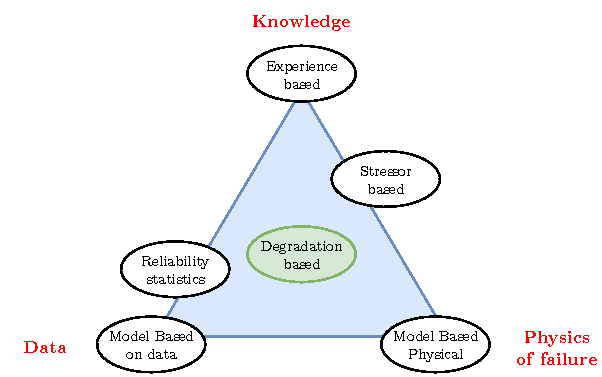
\includegraphics[scale=1.3]{images/Intro/MaintTriangle.pdf}
    \caption{Maintenance triangle}
    \label{fig:MaintTriangle}
\end{figure} 

Takin for example a survey published by the U.S. Department of Commerce in 2020, the maintenance expenditure of the manufacturing industry in the USA was \$57.3 billion, while the losses due to preventable maintenance issues amounted to \$119.1 billion. The top 25\% of those 
establishments relying on reactive maintenance were associated with 3.3 times more downtime 
than those in the bottom 25\% \cite{NIST}. This means that the economic impact of failures exceeds the cost of maintenance by a factor of 2.1, and this is concentrated in those sectors that rely more on reactive maintenance. The aforementioned emphasizes the importance of developing a general purpose \gls{pdm} system that can be applied in a large variety of systems.

In the article \cite{Maintenance_cat}, the authors divide the \gls{cbm} strategies in five categories:

\begin{itemize}
    \item \emph{experience based} predictions are based on the experience and knowledge outside or within the company. It is based on little scattered data on average conditions. The only  requirement is that the experience of the experts is quantified and used;
    \item \emph{reliability statistics} predictions are based on the statistical analysis of the failure data without considering the specific system. These methods also estimate the life
    of an average component operating under historically average conditions;
    \item \emph{stressor based} predictions can be considered an extension of the reliability statistics methods. The difference is that they also consider a measure of the stress (humidity, temperature, etc.) that the component is exposed to;
    \item \emph{degradation based} predictions are based on the extrapolation of the degradation of the component;
    \item \emph{model based} predictions are based on the knowledge of the physics of the system. The assumption is that the degradation can be computed instead of measured. They can be based on a physical model or on a data-driven model.
\end{itemize}


The authors of \cite{Maintenance_cat} also propose a distribution of these categories in a triangle, as shown in \autoref{fig:MaintTriangle}. Each vertex represents a requisite for the implementation, and the distance of the method to the vertex represents how dependent it is on that requisite. To obtain a general purpose \gls{pdm} framework, the \emph{degradation based} approach seems the most promising, since it is the least dependent on a specific requisite.

Moreover, to enhance even more the general purpose nature of the framework, a \gls{uml} model can be chosen. This speeds up the implementation of the framework on a machine about which little is known, plus, it can be implemented on a new machine without a deep knowledge of the \gls{uml} algorithms themself.

In the paper \cite{GridPredictMaintenance}, it is pointed out that \gls{glo:edge} implementations, not only enable the use of the framework for special applications but also enhance the cybersecurity of facilities that may not need an edge implementation due to technical limitations.
\section{Objective of the thesis}
\label{sec:objectives}

The goal of this thesis is to design, code and test a \gls{cbm} framework that will perform \gls{nd}, \gls{fd} and \gls{pdm}. This framework is thought to be general purpose, it needs just to receive time-series data from sensors, and set in training or evaluation mode.
This system will be implemented twice:
\begin{itemize}
    \item  coding in \texttt{python} and running it on a \gls{pc};
    \item   coding in \texttt{C} and running it on a microcontroller.
\end{itemize}

The development of the framework has been done modular and configurable, so that it can be easily adapted to different use cases. Things like the number of sensors, the sampling frequency, and the number and types of features to extract are easily configurable in a single file. The framework is also designed to be easily expandable, so that new features can be added simply by developing a method that appends the new feature to the feature vector, without the need to modify the rest of the framework.

To do that first a real bearing vibration dataset published by \cite{IMSpaper} has been analyzed to decide how to preprocess the data, which features to extract and which algorithm to use. 
The candidate algorithms described in \autoref{ch:Unsupervised} have been applied to the dataset and the results have been compared. These algorithms are \textbf{K-means}, \textbf{\gls{dbscan}}, \textbf{Gaussian Mixture Model}, \textbf{Isolation Forest}, \textbf{Local Outlier Factor} and \textbf{One-Class support vector machine}. 

All of the tests have been done trying to follow the most unsupervised approach possible, so the only information used to train the algorithm has been the data itself. Every user input needed by the algorithm has been chosen using an easily automatable method, to preserve the unsupervised nature of the framework that will be developed. For example, user inputs are the number of clusters in K-means, or the radius in the \gls{dbscan}.

At the end of the analysis, considering the trade-off between the performance of the algorithm, the computational cost and the simplicity, K-means has been chosen as the algorithm to implement in a real-time framework, developed in texttt{python}. Then, the data of the dataset was polled from a database at regular intervals and fed to the framework to simulate a real sensor polling the signal from the machine and evaluate the real-time performance of the implementation.

After that, a version of the framework with simplified architecture has been implemented in \texttt{C} and tested on a \texttt{STM32F767ZI} microcontroller board.

\section{Notations}
\label{sec:notations}
In this thesis, the following notations are used:
\begin{itemize}
  \item bold lowercase letters ($\vect{a}$, $\vect{b}$, $\vect{c}$) are used to denote vectors;
  \item italic lowercase letters ($a$, $b$, $c$) are used to denote scalars;
  \item bold uppercase letters ($\vect{A}$, $\vect{B}$, $\vect{C}$) are used to denote matrices;
  \item $\vect{a}_{i(j)}$ is the $j$th element of the vector $\vect{a}_i$;
  \item $||\vect{a}||_2$ is the $l^2$-norm of the vector $\vect{a}$, defined as $\sqrt{\sum_{i=1}^{n} a_i^2}$, denoted also as $\norm{a}$ for simplicity;
  \item $||\vect{a}||_n$ is the generic $l^n$-norm of the vector $\vect{a}$, defined as $\sqrt[n]{\sum_{i=1}^{n} \abs{a_i}^n}$;
  \item parenthesis encapsulating an index are used to condense descriptions, for example \quoted{\textbf{$\vect{a}_{i(j)}$ is the force applied to the $i$th ($j$th) step}} means that $\vect{a}_i$ is the force applied to the $i$th step and $\vect{a}_j$ is the force applied to the $j$th step;
  \item date and times are presented in the \gls{iso} 8601 format \cite{iso8601}. for example \texttt{YYYY-MM-DDThh:mm:ss}, where \texttt{T} is the date-time separator;
\end{itemize}

No distinction in notation is made between a vector in the phisycal sense (applied to a point, with a direction, and a magnitude) and a vector in the mathematical sense (a generic number $\in \mathbb{R}^n $).

As regard the flowcharts, the following symbols shown in \autoref{tab:flowsymbols} are used.


\begin{longtblr}[
  caption = {Symbols used in the flowcharts},
  label = {tab:flowsymbols},
]{
  cell{2}{1} = {t},
  cell{3}{1} = {t},
  cell{5}{1} = {t},
  cell{6}{1} = {t},
  cell{7}{1} = {t},
  hline{1,13} = {-}{0.08em},
  hline{2} = {-}{},
}
\textbf{Symbol} & \textbf{Name} & \textbf{Usage}\\
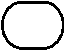
\includegraphics[scale=1]{images/FlowSymbols/terminator.pdf} & terminator & start or stop the process\\

\includegraphics[scale=1]{images/FlowSymbols/storedData.pdf} & stored data & save some data\\

\includegraphics[scale=1]{images/FlowSymbols/data.pdf} & data & elaborate some data\\

\includegraphics[scale=1]{images/FlowSymbols/process.pdf} & actions & perform automated actions\\

\includegraphics[scale=1]{images/FlowSymbols/document.pdf} & document & read or write a docuument\\
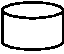
\includegraphics[scale=1]{images/FlowSymbols/database.pdf} & database & perform an action on a database\\

\includegraphics[scale=1]{images/FlowSymbols/display.pdf} & display & report, plot or display a value\\

\includegraphics[scale=1]{images/FlowSymbols/manualInput.pdf} & manual input & request an input from the user\\

\includegraphics[scale=1]{images/FlowSymbols/manualOperation.pdf} & manual operation & request the user to do something\\

\includegraphics[scale=1]{images/FlowSymbols/or.pdf} & or & join flow line\\
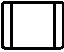
\includegraphics[scale=1]{images/FlowSymbols/predefProcess.pdf} & predefined process & run a programmed process
\end{longtblr}


%\printinunitsof{in}\prntlen{\textwidth}

% \begin{figure*}
%   \centering
% \begin{subfigure}{0.3\linewidth}  % <----
%  % This file was created with tikzplotlib v0.10.1.
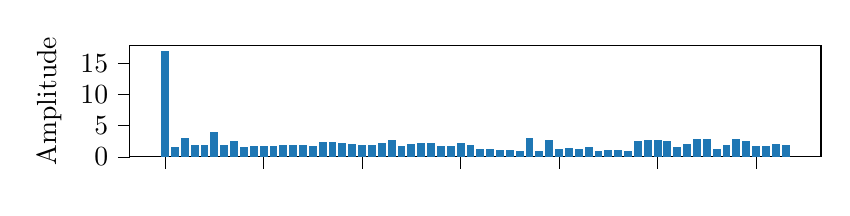
\begin{tikzpicture}

\definecolor{darkgray176}{RGB}{176,176,176}
\definecolor{steelblue31119180}{RGB}{31,119,180}

\begin{axis}[
height=3cm,
scaled x ticks=manual:{}{\pgfmathparse{#1}},
tick align=outside,
tick pos=left,
width=294.76926pt,
x grid style={darkgray176},
xmin=-3.59, xmax=66.59,
xtick style={color=black},
xticklabels={},
y grid style={darkgray176},
ylabel={Amplitude},
ymin=0, ymax=17.9224917606911,
ytick style={color=black},
ytick={0,5,10,15,20},
yticklabels={
  \(\displaystyle {0}\),
  \(\displaystyle {5}\),
  \(\displaystyle {10}\),
  \(\displaystyle {15}\),
  \(\displaystyle {20}\)
}
]
\draw[draw=none,fill=steelblue31119180] (axis cs:-0.4,0) rectangle (axis cs:0.4,17.0690397720867);
\draw[draw=none,fill=steelblue31119180] (axis cs:0.6,0) rectangle (axis cs:1.4,1.57701532870284);
\draw[draw=none,fill=steelblue31119180] (axis cs:1.6,0) rectangle (axis cs:2.4,3.04515592469192);
\draw[draw=none,fill=steelblue31119180] (axis cs:2.6,0) rectangle (axis cs:3.4,1.98727065046711);
\draw[draw=none,fill=steelblue31119180] (axis cs:3.6,0) rectangle (axis cs:4.4,1.87901229043815);
\draw[draw=none,fill=steelblue31119180] (axis cs:4.6,0) rectangle (axis cs:5.4,3.94494985947408);
\draw[draw=none,fill=steelblue31119180] (axis cs:5.6,0) rectangle (axis cs:6.4,1.94821362148988);
\draw[draw=none,fill=steelblue31119180] (axis cs:6.6,0) rectangle (axis cs:7.4,2.53456682074799);
\draw[draw=none,fill=steelblue31119180] (axis cs:7.6,0) rectangle (axis cs:8.4,1.53982779775888);
\draw[draw=none,fill=steelblue31119180] (axis cs:8.6,0) rectangle (axis cs:9.4,1.81855063876657);
\draw[draw=none,fill=steelblue31119180] (axis cs:9.6,0) rectangle (axis cs:10.4,1.74372106320514);
\draw[draw=none,fill=steelblue31119180] (axis cs:10.6,0) rectangle (axis cs:11.4,1.78981913351115);
\draw[draw=none,fill=steelblue31119180] (axis cs:11.6,0) rectangle (axis cs:12.4,1.9283565514217);
\draw[draw=none,fill=steelblue31119180] (axis cs:12.6,0) rectangle (axis cs:13.4,1.98727539890716);
\draw[draw=none,fill=steelblue31119180] (axis cs:13.6,0) rectangle (axis cs:14.4,1.83637697194901);
\draw[draw=none,fill=steelblue31119180] (axis cs:14.6,0) rectangle (axis cs:15.4,1.70629362470728);
\draw[draw=none,fill=steelblue31119180] (axis cs:15.6,0) rectangle (axis cs:16.4,2.32898911515285);
\draw[draw=none,fill=steelblue31119180] (axis cs:16.6,0) rectangle (axis cs:17.4,2.38726500121464);
\draw[draw=none,fill=steelblue31119180] (axis cs:17.6,0) rectangle (axis cs:18.4,2.2146470907513);
\draw[draw=none,fill=steelblue31119180] (axis cs:18.6,0) rectangle (axis cs:19.4,2.08886171015996);
\draw[draw=none,fill=steelblue31119180] (axis cs:19.6,0) rectangle (axis cs:20.4,1.91586717365543);
\draw[draw=none,fill=steelblue31119180] (axis cs:20.6,0) rectangle (axis cs:21.4,1.97741699428014);
\draw[draw=none,fill=steelblue31119180] (axis cs:21.6,0) rectangle (axis cs:22.4,2.26324345140917);
\draw[draw=none,fill=steelblue31119180] (axis cs:22.6,0) rectangle (axis cs:23.4,2.74150949309368);
\draw[draw=none,fill=steelblue31119180] (axis cs:23.6,0) rectangle (axis cs:24.4,1.67879784390802);
\draw[draw=none,fill=steelblue31119180] (axis cs:24.6,0) rectangle (axis cs:25.4,1.99560308046926);
\draw[draw=none,fill=steelblue31119180] (axis cs:25.6,0) rectangle (axis cs:26.4,2.18236194366914);
\draw[draw=none,fill=steelblue31119180] (axis cs:26.6,0) rectangle (axis cs:27.4,2.28116664486001);
\draw[draw=none,fill=steelblue31119180] (axis cs:27.6,0) rectangle (axis cs:28.4,1.76545125094874);
\draw[draw=none,fill=steelblue31119180] (axis cs:28.6,0) rectangle (axis cs:29.4,1.79936118428771);
\draw[draw=none,fill=steelblue31119180] (axis cs:29.6,0) rectangle (axis cs:30.4,2.21046386064049);
\draw[draw=none,fill=steelblue31119180] (axis cs:30.6,0) rectangle (axis cs:31.4,1.92512684988102);
\draw[draw=none,fill=steelblue31119180] (axis cs:31.6,0) rectangle (axis cs:32.4,1.29434219923151);
\draw[draw=none,fill=steelblue31119180] (axis cs:32.6,0) rectangle (axis cs:33.4,1.24905838096159);
\draw[draw=none,fill=steelblue31119180] (axis cs:33.6,0) rectangle (axis cs:34.4,1.0539404131426);
\draw[draw=none,fill=steelblue31119180] (axis cs:34.6,0) rectangle (axis cs:35.4,1.07785302549105);
\draw[draw=none,fill=steelblue31119180] (axis cs:35.6,0) rectangle (axis cs:36.4,1.00170991631713);
\draw[draw=none,fill=steelblue31119180] (axis cs:36.6,0) rectangle (axis cs:37.4,2.990570610034);
\draw[draw=none,fill=steelblue31119180] (axis cs:37.6,0) rectangle (axis cs:38.4,1.00976749017216);
\draw[draw=none,fill=steelblue31119180] (axis cs:38.6,0) rectangle (axis cs:39.4,2.77121989223762);
\draw[draw=none,fill=steelblue31119180] (axis cs:39.6,0) rectangle (axis cs:40.4,1.21267465980989);
\draw[draw=none,fill=steelblue31119180] (axis cs:40.6,0) rectangle (axis cs:41.4,1.44620941204964);
\draw[draw=none,fill=steelblue31119180] (axis cs:41.6,0) rectangle (axis cs:42.4,1.26138331095181);
\draw[draw=none,fill=steelblue31119180] (axis cs:42.6,0) rectangle (axis cs:43.4,1.60664374136418);
\draw[draw=none,fill=steelblue31119180] (axis cs:43.6,0) rectangle (axis cs:44.4,0.883196382772003);
\draw[draw=none,fill=steelblue31119180] (axis cs:44.6,0) rectangle (axis cs:45.4,1.0835546712407);
\draw[draw=none,fill=steelblue31119180] (axis cs:45.6,0) rectangle (axis cs:46.4,1.05267232084);
\draw[draw=none,fill=steelblue31119180] (axis cs:46.6,0) rectangle (axis cs:47.4,0.94061509525324);
\draw[draw=none,fill=steelblue31119180] (axis cs:47.6,0) rectangle (axis cs:48.4,2.5937245360833);
\draw[draw=none,fill=steelblue31119180] (axis cs:48.6,0) rectangle (axis cs:49.4,2.7964850933437);
\draw[draw=none,fill=steelblue31119180] (axis cs:49.6,0) rectangle (axis cs:50.4,2.71286149748853);
\draw[draw=none,fill=steelblue31119180] (axis cs:50.6,0) rectangle (axis cs:51.4,2.61834135486071);
\draw[draw=none,fill=steelblue31119180] (axis cs:51.6,0) rectangle (axis cs:52.4,1.64261763713365);
\draw[draw=none,fill=steelblue31119180] (axis cs:52.6,0) rectangle (axis cs:53.4,2.10765089952882);
\draw[draw=none,fill=steelblue31119180] (axis cs:53.6,0) rectangle (axis cs:54.4,2.79833649937833);
\draw[draw=none,fill=steelblue31119180] (axis cs:54.6,0) rectangle (axis cs:55.4,2.89223762573101);
\draw[draw=none,fill=steelblue31119180] (axis cs:55.6,0) rectangle (axis cs:56.4,1.32361974945306);
\draw[draw=none,fill=steelblue31119180] (axis cs:56.6,0) rectangle (axis cs:57.4,1.84030534558782);
\draw[draw=none,fill=steelblue31119180] (axis cs:57.6,0) rectangle (axis cs:58.4,2.82922380450697);
\draw[draw=none,fill=steelblue31119180] (axis cs:58.6,0) rectangle (axis cs:59.4,2.5822341294544);
\draw[draw=none,fill=steelblue31119180] (axis cs:59.6,0) rectangle (axis cs:60.4,1.71682916120663);
\draw[draw=none,fill=steelblue31119180] (axis cs:60.6,0) rectangle (axis cs:61.4,1.73398491114388);
\draw[draw=none,fill=steelblue31119180] (axis cs:61.6,0) rectangle (axis cs:62.4,2.13866133729592);
\draw[draw=none,fill=steelblue31119180] (axis cs:62.6,0) rectangle (axis cs:63.4,1.90570304888095);
\end{axis}

\end{tikzpicture}

%  \caption{Model 1}
%  \label{fig1a}
% \end{subfigure}

% \begin{subfigure}{0.3\linewidth}  % <----
%  % This file was created with tikzplotlib v0.10.1.
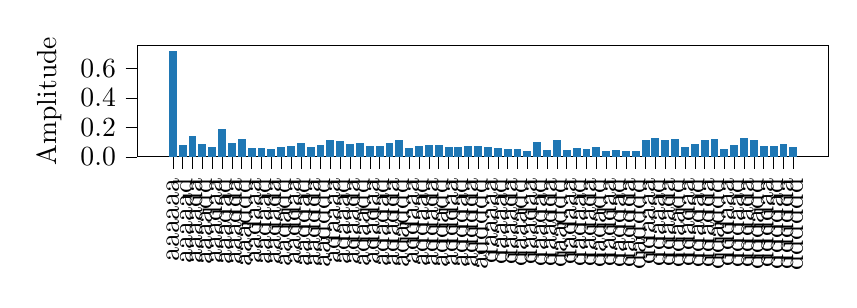
\begin{tikzpicture}

\definecolor{darkgray176}{RGB}{176,176,176}
\definecolor{steelblue31119180}{RGB}{31,119,180}

\begin{axis}[
height=3cm,
tick align=outside,
tick pos=left,
width=294.76926pt,
x grid style={darkgray176},
xmin=-3.59, xmax=66.59,
xtick style={color=black},
xtick={0,1,2,3,4,5,6,7,8,9,10,11,12,13,14,15,16,17,18,19,20,21,22,23,24,25,26,27,28,29,30,31,32,33,34,35,36,37,38,39,40,41,42,43,44,45,46,47,48,49,50,51,52,53,54,55,56,57,58,59,60,61,62,63},
xticklabel style={rotate=90.0},
xticklabels={
  aaaaaa,
  aaaaad,
  aaaada,
  aaaadd,
  aaadaa,
  aaadad,
  aaadda,
  aaaddd,
  aadaaa,
  aadaad,
  aadada,
  aadadd,
  aaddaa,
  aaddad,
  aaddda,
  aadddd,
  adaaaa,
  adaaad,
  adaada,
  adaadd,
  adadaa,
  adadad,
  adadda,
  adaddd,
  addaaa,
  addaad,
  addada,
  addadd,
  adddaa,
  adddad,
  adddda,
  addddd,
  daaaaa,
  daaaad,
  daaada,
  daaadd,
  daadaa,
  daadad,
  daadda,
  daaddd,
  dadaaa,
  dadaad,
  dadada,
  dadadd,
  daddaa,
  daddad,
  daddda,
  dadddd,
  ddaaaa,
  ddaaad,
  ddaada,
  ddaadd,
  ddadaa,
  ddadad,
  ddadda,
  ddaddd,
  dddaaa,
  dddaad,
  dddada,
  dddadd,
  ddddaa,
  ddddad,
  ddddda,
  dddddd
},
y grid style={darkgray176},
ylabel={Amplitude},
ymin=0, ymax=0.758179630791467,
ytick style={color=black},
ytick={0,0.2,0.4,0.6,0.8},
yticklabels={
  \(\displaystyle {0.0}\),
  \(\displaystyle {0.2}\),
  \(\displaystyle {0.4}\),
  \(\displaystyle {0.6}\),
  \(\displaystyle {0.8}\)
}
]
\draw[draw=none,fill=steelblue31119180] (axis cs:-0.4,0) rectangle (axis cs:0.4,0.722075838849016);
\draw[draw=none,fill=steelblue31119180] (axis cs:0.6,0) rectangle (axis cs:1.4,0.0816205118704516);
\draw[draw=none,fill=steelblue31119180] (axis cs:1.6,0) rectangle (axis cs:2.4,0.144788692125759);
\draw[draw=none,fill=steelblue31119180] (axis cs:2.6,0) rectangle (axis cs:3.4,0.0867045957893479);
\draw[draw=none,fill=steelblue31119180] (axis cs:3.6,0) rectangle (axis cs:4.4,0.0687644637243896);
\draw[draw=none,fill=steelblue31119180] (axis cs:4.6,0) rectangle (axis cs:5.4,0.191603550445973);
\draw[draw=none,fill=steelblue31119180] (axis cs:5.6,0) rectangle (axis cs:6.4,0.0912400814435433);
\draw[draw=none,fill=steelblue31119180] (axis cs:6.6,0) rectangle (axis cs:7.4,0.118441738979468);
\draw[draw=none,fill=steelblue31119180] (axis cs:7.6,0) rectangle (axis cs:8.4,0.063448949683056);
\draw[draw=none,fill=steelblue31119180] (axis cs:8.6,0) rectangle (axis cs:9.4,0.063549196660358);
\draw[draw=none,fill=steelblue31119180] (axis cs:9.6,0) rectangle (axis cs:10.4,0.0561566529115002);
\draw[draw=none,fill=steelblue31119180] (axis cs:10.6,0) rectangle (axis cs:11.4,0.0658459782078631);
\draw[draw=none,fill=steelblue31119180] (axis cs:11.6,0) rectangle (axis cs:12.4,0.0720379897131174);
\draw[draw=none,fill=steelblue31119180] (axis cs:12.6,0) rectangle (axis cs:13.4,0.0962993461770895);
\draw[draw=none,fill=steelblue31119180] (axis cs:13.6,0) rectangle (axis cs:14.4,0.0686195486369405);
\draw[draw=none,fill=steelblue31119180] (axis cs:14.6,0) rectangle (axis cs:15.4,0.0841955303823389);
\draw[draw=none,fill=steelblue31119180] (axis cs:15.6,0) rectangle (axis cs:16.4,0.114948175605847);
\draw[draw=none,fill=steelblue31119180] (axis cs:16.6,0) rectangle (axis cs:17.4,0.111103219250477);
\draw[draw=none,fill=steelblue31119180] (axis cs:17.6,0) rectangle (axis cs:18.4,0.0853474774953162);
\draw[draw=none,fill=steelblue31119180] (axis cs:18.6,0) rectangle (axis cs:19.4,0.0954229864952013);
\draw[draw=none,fill=steelblue31119180] (axis cs:19.6,0) rectangle (axis cs:20.4,0.0753330666191015);
\draw[draw=none,fill=steelblue31119180] (axis cs:20.6,0) rectangle (axis cs:21.4,0.0764573561609443);
\draw[draw=none,fill=steelblue31119180] (axis cs:21.6,0) rectangle (axis cs:22.4,0.0913486161286602);
\draw[draw=none,fill=steelblue31119180] (axis cs:22.6,0) rectangle (axis cs:23.4,0.115440781780618);
\draw[draw=none,fill=steelblue31119180] (axis cs:23.6,0) rectangle (axis cs:24.4,0.0605363919448476);
\draw[draw=none,fill=steelblue31119180] (axis cs:24.6,0) rectangle (axis cs:25.4,0.0715006546875076);
\draw[draw=none,fill=steelblue31119180] (axis cs:25.6,0) rectangle (axis cs:26.4,0.0834816059877538);
\draw[draw=none,fill=steelblue31119180] (axis cs:26.6,0) rectangle (axis cs:27.4,0.0825718187220844);
\draw[draw=none,fill=steelblue31119180] (axis cs:27.6,0) rectangle (axis cs:28.4,0.0657381299772261);
\draw[draw=none,fill=steelblue31119180] (axis cs:28.6,0) rectangle (axis cs:29.4,0.0684981211033183);
\draw[draw=none,fill=steelblue31119180] (axis cs:29.6,0) rectangle (axis cs:30.4,0.0735247581287173);
\draw[draw=none,fill=steelblue31119180] (axis cs:30.6,0) rectangle (axis cs:31.4,0.0714264975904106);
\draw[draw=none,fill=steelblue31119180] (axis cs:31.6,0) rectangle (axis cs:32.4,0.0674403501539547);
\draw[draw=none,fill=steelblue31119180] (axis cs:32.6,0) rectangle (axis cs:33.4,0.0592824747919798);
\draw[draw=none,fill=steelblue31119180] (axis cs:33.6,0) rectangle (axis cs:34.4,0.052030899559776);
\draw[draw=none,fill=steelblue31119180] (axis cs:34.6,0) rectangle (axis cs:35.4,0.0513258807665482);
\draw[draw=none,fill=steelblue31119180] (axis cs:35.6,0) rectangle (axis cs:36.4,0.0416017100177299);
\draw[draw=none,fill=steelblue31119180] (axis cs:36.6,0) rectangle (axis cs:37.4,0.101744455756126);
\draw[draw=none,fill=steelblue31119180] (axis cs:37.6,0) rectangle (axis cs:38.4,0.0463410493438625);
\draw[draw=none,fill=steelblue31119180] (axis cs:38.6,0) rectangle (axis cs:39.4,0.117328390407309);
\draw[draw=none,fill=steelblue31119180] (axis cs:39.6,0) rectangle (axis cs:40.4,0.0462494158731625);
\draw[draw=none,fill=steelblue31119180] (axis cs:40.6,0) rectangle (axis cs:41.4,0.0593257131667686);
\draw[draw=none,fill=steelblue31119180] (axis cs:41.6,0) rectangle (axis cs:42.4,0.0526934179057522);
\draw[draw=none,fill=steelblue31119180] (axis cs:42.6,0) rectangle (axis cs:43.4,0.0668781753176304);
\draw[draw=none,fill=steelblue31119180] (axis cs:43.6,0) rectangle (axis cs:44.4,0.0416416018534089);
\draw[draw=none,fill=steelblue31119180] (axis cs:44.6,0) rectangle (axis cs:45.4,0.0462760456257271);
\draw[draw=none,fill=steelblue31119180] (axis cs:45.6,0) rectangle (axis cs:46.4,0.0434239384103015);
\draw[draw=none,fill=steelblue31119180] (axis cs:46.6,0) rectangle (axis cs:47.4,0.0416410127228071);
\draw[draw=none,fill=steelblue31119180] (axis cs:47.6,0) rectangle (axis cs:48.4,0.117322919554115);
\draw[draw=none,fill=steelblue31119180] (axis cs:48.6,0) rectangle (axis cs:49.4,0.130187409367646);
\draw[draw=none,fill=steelblue31119180] (axis cs:49.6,0) rectangle (axis cs:50.4,0.114133627497582);
\draw[draw=none,fill=steelblue31119180] (axis cs:50.6,0) rectangle (axis cs:51.4,0.121358917513582);
\draw[draw=none,fill=steelblue31119180] (axis cs:51.6,0) rectangle (axis cs:52.4,0.0707478156876725);
\draw[draw=none,fill=steelblue31119180] (axis cs:52.6,0) rectangle (axis cs:53.4,0.0878711098289786);
\draw[draw=none,fill=steelblue31119180] (axis cs:53.6,0) rectangle (axis cs:54.4,0.112974228550204);
\draw[draw=none,fill=steelblue31119180] (axis cs:54.6,0) rectangle (axis cs:55.4,0.120443137445082);
\draw[draw=none,fill=steelblue31119180] (axis cs:55.6,0) rectangle (axis cs:56.4,0.053252675940857);
\draw[draw=none,fill=steelblue31119180] (axis cs:56.6,0) rectangle (axis cs:57.4,0.077975346334595);
\draw[draw=none,fill=steelblue31119180] (axis cs:57.6,0) rectangle (axis cs:58.4,0.125489421529731);
\draw[draw=none,fill=steelblue31119180] (axis cs:58.6,0) rectangle (axis cs:59.4,0.113761107750516);
\draw[draw=none,fill=steelblue31119180] (axis cs:59.6,0) rectangle (axis cs:60.4,0.0721800422035524);
\draw[draw=none,fill=steelblue31119180] (axis cs:60.6,0) rectangle (axis cs:61.4,0.0753054888730634);
\draw[draw=none,fill=steelblue31119180] (axis cs:61.6,0) rectangle (axis cs:62.4,0.0854419009187501);
\draw[draw=none,fill=steelblue31119180] (axis cs:62.6,0) rectangle (axis cs:63.4,0.0676569727174981);
\end{axis}

\end{tikzpicture}

%  \caption{Model 2}
%  \label{fig1b}
% \end{subfigure}

% \begin{subfigure}{0.3\linewidth}  % <----
%  % This file was created with tikzplotlib v0.10.1.
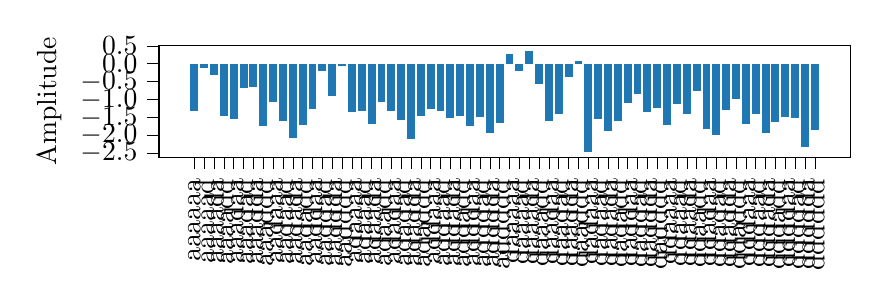
\begin{tikzpicture}

\definecolor{darkgray176}{RGB}{176,176,176}
\definecolor{steelblue31119180}{RGB}{31,119,180}

\begin{axis}[
height=3cm,
tick align=outside,
tick pos=left,
width=294.76926pt,
x grid style={darkgray176},
xmin=-3.59, xmax=66.59,
xtick style={color=black},
xtick={0,1,2,3,4,5,6,7,8,9,10,11,12,13,14,15,16,17,18,19,20,21,22,23,24,25,26,27,28,29,30,31,32,33,34,35,36,37,38,39,40,41,42,43,44,45,46,47,48,49,50,51,52,53,54,55,56,57,58,59,60,61,62,63},
xticklabel style={rotate=90.0},
xticklabels={
  aaaaaa,
  aaaaad,
  aaaada,
  aaaadd,
  aaadaa,
  aaadad,
  aaadda,
  aaaddd,
  aadaaa,
  aadaad,
  aadada,
  aadadd,
  aaddaa,
  aaddad,
  aaddda,
  aadddd,
  adaaaa,
  adaaad,
  adaada,
  adaadd,
  adadaa,
  adadad,
  adadda,
  adaddd,
  addaaa,
  addaad,
  addada,
  addadd,
  adddaa,
  adddad,
  adddda,
  addddd,
  daaaaa,
  daaaad,
  daaada,
  daaadd,
  daadaa,
  daadad,
  daadda,
  daaddd,
  dadaaa,
  dadaad,
  dadada,
  dadadd,
  daddaa,
  daddad,
  daddda,
  dadddd,
  ddaaaa,
  ddaaad,
  ddaada,
  ddaadd,
  ddadaa,
  ddadad,
  ddadda,
  ddaddd,
  dddaaa,
  dddaad,
  dddada,
  dddadd,
  ddddaa,
  ddddad,
  ddddda,
  dddddd
},
y grid style={darkgray176},
ylabel={Amplitude},
ymin=-2.61740256008719, ymax=0.509919465810349,
ytick style={color=black},
ytick={-3,-2.5,-2,-1.5,-1,-0.5,0,0.5,1},
yticklabels={
  \(\displaystyle {\ensuremath{-}3.0}\),
  \(\displaystyle {\ensuremath{-}2.5}\),
  \(\displaystyle {\ensuremath{-}2.0}\),
  \(\displaystyle {\ensuremath{-}1.5}\),
  \(\displaystyle {\ensuremath{-}1.0}\),
  \(\displaystyle {\ensuremath{-}0.5}\),
  \(\displaystyle {0.0}\),
  \(\displaystyle {0.5}\),
  \(\displaystyle {1.0}\)
}
]
\draw[draw=none,fill=steelblue31119180] (axis cs:-0.4,0) rectangle (axis cs:0.4,-1.31463451570886);
\draw[draw=none,fill=steelblue31119180] (axis cs:0.6,0) rectangle (axis cs:1.4,-0.134818691790791);
\draw[draw=none,fill=steelblue31119180] (axis cs:1.6,0) rectangle (axis cs:2.4,-0.319435036080992);
\draw[draw=none,fill=steelblue31119180] (axis cs:2.6,0) rectangle (axis cs:3.4,-1.45257985930736);
\draw[draw=none,fill=steelblue31119180] (axis cs:3.6,0) rectangle (axis cs:4.4,-1.5421469645371);
\draw[draw=none,fill=steelblue31119180] (axis cs:4.6,0) rectangle (axis cs:5.4,-0.673764853725896);
\draw[draw=none,fill=steelblue31119180] (axis cs:5.6,0) rectangle (axis cs:6.4,-0.651067231629759);
\draw[draw=none,fill=steelblue31119180] (axis cs:6.6,0) rectangle (axis cs:7.4,-1.74945636196658);
\draw[draw=none,fill=steelblue31119180] (axis cs:7.6,0) rectangle (axis cs:8.4,-1.07894447704247);
\draw[draw=none,fill=steelblue31119180] (axis cs:8.6,0) rectangle (axis cs:9.4,-1.611860529353);
\draw[draw=none,fill=steelblue31119180] (axis cs:9.6,0) rectangle (axis cs:10.4,-2.08587288612999);
\draw[draw=none,fill=steelblue31119180] (axis cs:10.6,0) rectangle (axis cs:11.4,-1.70951336361917);
\draw[draw=none,fill=steelblue31119180] (axis cs:11.6,0) rectangle (axis cs:12.4,-1.28157675228911);
\draw[draw=none,fill=steelblue31119180] (axis cs:12.6,0) rectangle (axis cs:13.4,-0.197861624149187);
\draw[draw=none,fill=steelblue31119180] (axis cs:13.6,0) rectangle (axis cs:14.4,-0.902246969989867);
\draw[draw=none,fill=steelblue31119180] (axis cs:14.6,0) rectangle (axis cs:15.4,-0.0599945188814577);
\draw[draw=none,fill=steelblue31119180] (axis cs:15.6,0) rectangle (axis cs:16.4,-1.36541350319367);
\draw[draw=none,fill=steelblue31119180] (axis cs:16.6,0) rectangle (axis cs:17.4,-1.3266188419031);
\draw[draw=none,fill=steelblue31119180] (axis cs:17.6,0) rectangle (axis cs:18.4,-1.69808295679741);
\draw[draw=none,fill=steelblue31119180] (axis cs:18.6,0) rectangle (axis cs:19.4,-1.08150865222734);
\draw[draw=none,fill=steelblue31119180] (axis cs:19.6,0) rectangle (axis cs:20.4,-1.3300365540605);
\draw[draw=none,fill=steelblue31119180] (axis cs:20.6,0) rectangle (axis cs:21.4,-1.56591194958796);
\draw[draw=none,fill=steelblue31119180] (axis cs:21.6,0) rectangle (axis cs:22.4,-2.10018255300044);
\draw[draw=none,fill=steelblue31119180] (axis cs:22.6,0) rectangle (axis cs:23.4,-1.46373211270423);
\draw[draw=none,fill=steelblue31119180] (axis cs:23.6,0) rectangle (axis cs:24.4,-1.27545670892696);
\draw[draw=none,fill=steelblue31119180] (axis cs:24.6,0) rectangle (axis cs:25.4,-1.33850245699865);
\draw[draw=none,fill=steelblue31119180] (axis cs:25.6,0) rectangle (axis cs:26.4,-1.52906230329855);
\draw[draw=none,fill=steelblue31119180] (axis cs:26.6,0) rectangle (axis cs:27.4,-1.45230662679311);
\draw[draw=none,fill=steelblue31119180] (axis cs:27.6,0) rectangle (axis cs:28.4,-1.73255965580102);
\draw[draw=none,fill=steelblue31119180] (axis cs:28.6,0) rectangle (axis cs:29.4,-1.50335007709024);
\draw[draw=none,fill=steelblue31119180] (axis cs:29.6,0) rectangle (axis cs:30.4,-1.94720337219532);
\draw[draw=none,fill=steelblue31119180] (axis cs:30.6,0) rectangle (axis cs:31.4,-1.65528675483821);
\draw[draw=none,fill=steelblue31119180] (axis cs:31.6,0) rectangle (axis cs:32.4,0.270054443767034);
\draw[draw=none,fill=steelblue31119180] (axis cs:32.6,0) rectangle (axis cs:33.4,-0.197751373312009);
\draw[draw=none,fill=steelblue31119180] (axis cs:33.6,0) rectangle (axis cs:34.4,0.367768464633188);
\draw[draw=none,fill=steelblue31119180] (axis cs:34.6,0) rectangle (axis cs:35.4,-0.564735648791296);
\draw[draw=none,fill=steelblue31119180] (axis cs:35.6,0) rectangle (axis cs:36.4,-1.61150252577791);
\draw[draw=none,fill=steelblue31119180] (axis cs:36.6,0) rectangle (axis cs:37.4,-1.40564010823609);
\draw[draw=none,fill=steelblue31119180] (axis cs:37.6,0) rectangle (axis cs:38.4,-0.371182760704031);
\draw[draw=none,fill=steelblue31119180] (axis cs:38.6,0) rectangle (axis cs:39.4,0.070349641149425);
\draw[draw=none,fill=steelblue31119180] (axis cs:39.6,0) rectangle (axis cs:40.4,-2.47525155891003);
\draw[draw=none,fill=steelblue31119180] (axis cs:40.6,0) rectangle (axis cs:41.4,-1.55614989351769);
\draw[draw=none,fill=steelblue31119180] (axis cs:41.6,0) rectangle (axis cs:42.4,-1.88234123808839);
\draw[draw=none,fill=steelblue31119180] (axis cs:42.6,0) rectangle (axis cs:43.4,-1.59270070771934);
\draw[draw=none,fill=steelblue31119180] (axis cs:43.6,0) rectangle (axis cs:44.4,-1.11190650381437);
\draw[draw=none,fill=steelblue31119180] (axis cs:44.6,0) rectangle (axis cs:45.4,-0.840681397994204);
\draw[draw=none,fill=steelblue31119180] (axis cs:45.6,0) rectangle (axis cs:46.4,-1.34368535787999);
\draw[draw=none,fill=steelblue31119180] (axis cs:46.6,0) rectangle (axis cs:47.4,-1.25517956985282);
\draw[draw=none,fill=steelblue31119180] (axis cs:47.6,0) rectangle (axis cs:48.4,-1.7101579930862);
\draw[draw=none,fill=steelblue31119180] (axis cs:48.6,0) rectangle (axis cs:49.4,-1.14244936083466);
\draw[draw=none,fill=steelblue31119180] (axis cs:49.6,0) rectangle (axis cs:50.4,-1.41050679464651);
\draw[draw=none,fill=steelblue31119180] (axis cs:50.6,0) rectangle (axis cs:51.4,-0.772205746905425);
\draw[draw=none,fill=steelblue31119180] (axis cs:51.6,0) rectangle (axis cs:52.4,-1.82325501180065);
\draw[draw=none,fill=steelblue31119180] (axis cs:52.6,0) rectangle (axis cs:53.4,-1.99315327974258);
\draw[draw=none,fill=steelblue31119180] (axis cs:53.6,0) rectangle (axis cs:54.4,-1.29641163379117);
\draw[draw=none,fill=steelblue31119180] (axis cs:54.6,0) rectangle (axis cs:55.4,-0.990550307115663);
\draw[draw=none,fill=steelblue31119180] (axis cs:55.6,0) rectangle (axis cs:56.4,-1.6980346169395);
\draw[draw=none,fill=steelblue31119180] (axis cs:56.6,0) rectangle (axis cs:57.4,-1.42284013393087);
\draw[draw=none,fill=steelblue31119180] (axis cs:57.6,0) rectangle (axis cs:58.4,-1.94315047574371);
\draw[draw=none,fill=steelblue31119180] (axis cs:58.6,0) rectangle (axis cs:59.4,-1.62789056222075);
\draw[draw=none,fill=steelblue31119180] (axis cs:59.6,0) rectangle (axis cs:60.4,-1.48520306606731);
\draw[draw=none,fill=steelblue31119180] (axis cs:60.6,0) rectangle (axis cs:61.4,-1.50855956912423);
\draw[draw=none,fill=steelblue31119180] (axis cs:61.6,0) rectangle (axis cs:62.4,-2.32843343387864);
\draw[draw=none,fill=steelblue31119180] (axis cs:62.6,0) rectangle (axis cs:63.4,-1.84413382243553);
\end{axis}

\end{tikzpicture}

%  \caption{Model 2}
%  \label{fig1b}
% \end{subfigure}

% \caption{Models}
% \label{fig2}
% \end{figure*}

% \begin{figure}[htbp]
%   \centering
%   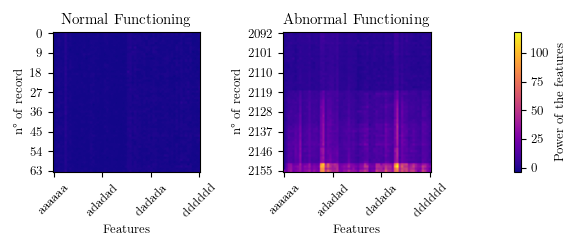
\includegraphics[scale=0.9]{images/Figure_5.png}
% \caption{Heatmap of the wavelet coefficients powers }
% \label{fig2}
% \end{figure}

% \begin{figure}[htbp]
%   \centering
%   \includesvg[width=\textwidth]{images/PMA_flowchart.svg}
% \caption{Predictive maintenance agent flowchart}
% \label{fig2}
% \end{figure}

% \begin{figure}[htbp]
%   \centering
%   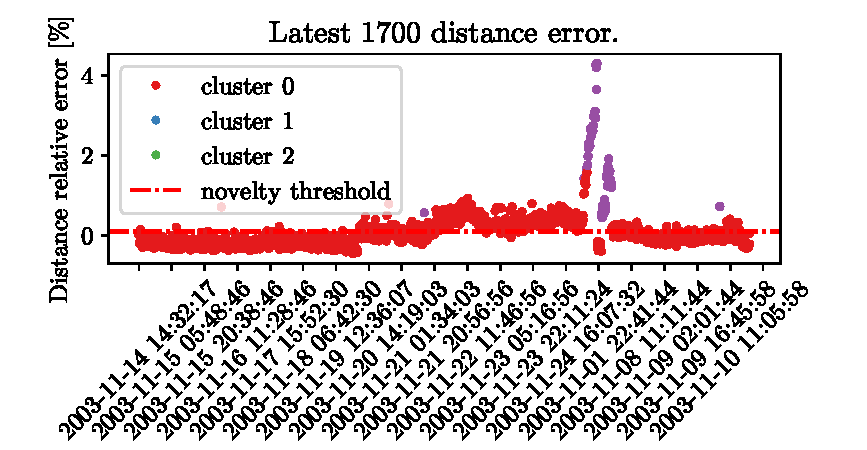
\includegraphics{images/Figure_1.pdf}
% \caption{Predictive maintenance agent flowchart}
% \label{fig2}
% \end{figure}}
\mask{\chapter{State of the Art}
\label{ch:state_of_the_art}

\begin{figure}[h]
    \centering
    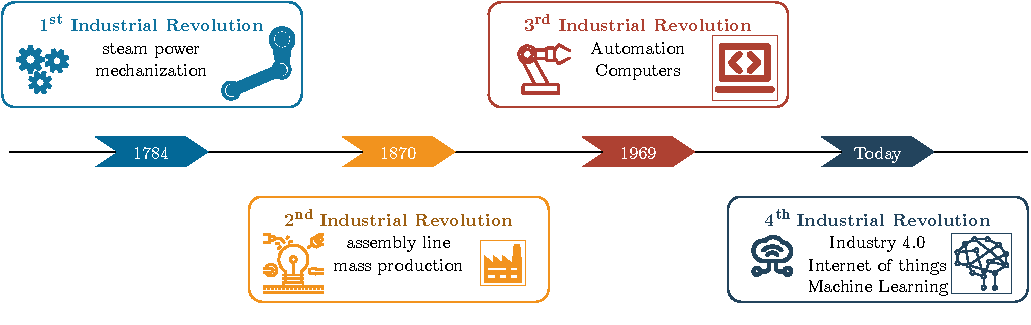
\includegraphics[width=\textwidth]{images/StateArt/Industry40.pdf}
    \caption{Industrial revolutions}
    \label{fig:ind40}    
\end{figure}

The invention of the modern steam engine in the $18^{th}$ century marked the beginning of the first industrial revolution. The second industrial revolution, in the $19^{th}$ century, was characterized by the introduction of mass production and the assembly line. The introduction of computers and automation in factories, in the $20^{th}$ century, enabled the third industrial revolution. Nowadays, we are currently living in the $4^{th}$ industrial revolution, that embraces the industry $4.0$ vision. State-of-the-art industries have small decentralized smart networks that make decisions autonomously. This is possible thanks to the \emph{Internet of Things} (\gls{iot}), smart sensors and actuators, and \emph{Big Data} analysis (\autoref{fig:ind40}). 
The data to be monitored varies \gls{wrt} the field of application. The most common are \cite{State_Art_Coanda_2020}:
\begin{itemize}
    \item Vibration Analysis - Efficient method for detecting issues in rotating equipment.
    \item Acoustic Analysis - Detects or monitors cracks in pipes and other structures.
    \item Lubrication Oils Analysis - Analyzes particles in oils to assess component wear.
    \item Particle Analysis in Working Environment - Applied to equipment operating in fluid environments.
    \item Corrosive Analysis - Ultrasound measurements to determine corrosion in various structures.
    \item Thermal Analysis - Identifies overheating in mechanical and electrical systems.
    \item Performance Analysis - Efficient technique for pinpointing operational problems in the system.
\end{itemize}



\paragraph{Standard terminology}
\begin{figure}
    \centering
    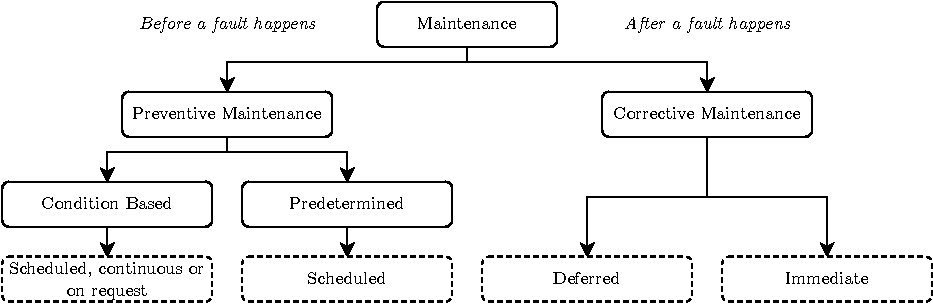
\includegraphics[width=\textwidth]{images/StateArt/EN_classification.drawio.pdf}
    \caption{Standard terminology for industrial maintenance \cite{rastegari2017condition}}
    \label{fig:standard_terminology}
\end{figure}

A standard terminology used for industrial maintenance is provided by the European committee for standardization with the standard \texttt{EN13306:2018} \cite{EN13306:2018}. The terminology is summarized in \autoref{fig:standard_terminology}. The most advanced maintenance technique family is \textbf{\gls{glo:conditionbasedmaintenance}}. This category includes the most modern \textbf{\gls{glo:predictivemaintenance}}. Note that the definition does not imply that the \quoted{monitoring} of the system must be continuous, it may also be scheduled or not even scheduled and performed both manually or by a program.

The standard also defines what \textbf{\gls{glo:onlinemaintenance}} and \textbf{\gls{glo:onistemaintenance}}. All these definitions are reported in the {glossary}.


\paragraph{\gls{rm} vs \gls{pm}}
\begin{figure}
    \centering
    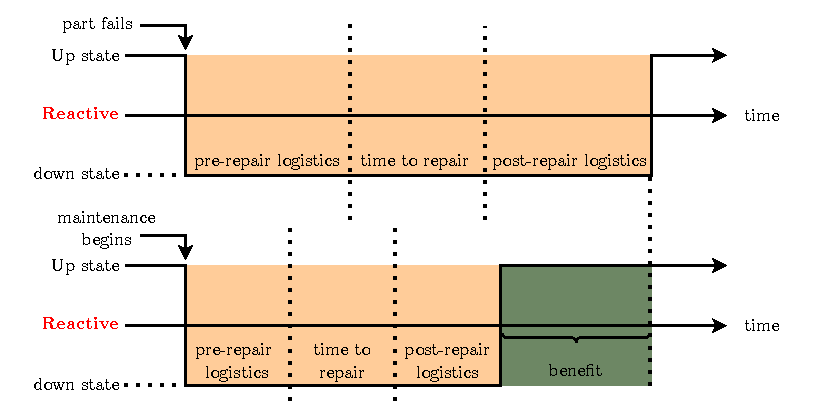
\includegraphics[width=\textwidth]{images/StateArt/lost_opportunities.pdf}
    \caption{Downtime comparison (\gls{rm} and \gls{pm})}
    \label{fig:lost_opportunities}
\end{figure}

As anticipated in the introduction, the two main approaches are \textbf{Reactive Maintenance} (\gls{aka} \gls{glo:correctivemaintenance}), which restores system functionality, and \textbf{Proactive Maintenance} (\gls{aka} \gls{glo:preventivemaintenance}), which preserves system functionality \cite{Rely_maint_book}.

The former approach leads to very high downtime \gls{wrt} the latter \cite{NIST}. For all the time a system is down, the company forfeits the opportunity to make a profit. This is called \emph{lost opportunity cost}. In reality, the total costs of downtime are even higher, because there are other costs associated with labor overhead and materials \cite{Lost_Opport_Cost}. The second approach optimizes both the pre-repair and post-repair logistics and, acting before the failure, can reduce also the total downtime. A qualitative diagram of these benefits is shown in \autoref{fig:lost_opportunities}. Other than the downtime, a more complete comparison between the advantages and disadvantages of the two approaches is shown in \autoref{tab:PM_vs_RM}.

% \usepackage{array}
% \usepackage{booktabs}


\begin{table}
    \centering
    \caption{Advantages and disadvantages of \gls{rm} and \gls{pm} maintenance \cite{Lost_Opport_Cost}}
    \resizebox{0.999999\textwidth}{!}{%
    \begin{tabular}{>{\hspace{0pt}}m{0.2\linewidth}>{\hspace{0pt}}m{0.344\linewidth}>{\hspace{0pt}}m{0.39\linewidth}} 
    \toprule
    \textbf{Maintenance} & \textbf{Advantages}                                                                                                                                                                                                                                                                                                                                                                                                                                                                                                                                                                                                                                                                                                                                                                                                                                                                                                                                  & \textbf{Disadvantages}                                                                                                                                                                                                               \\ 
    \hline
    Reactive             & \begin{tabular}{@{\labelitemi\hspace{\dimexpr\labelsep+0.5\tabcolsep}}l@{}}low setup cost\\easy to setup\end{tabular}                                                                                                                                                                                                                                                                                                                                                                                                                                                                                                                                                                                                                                                                                                                                                                                                                                & \begin{tabular}{@{\labelitemi\hspace{\dimexpr\labelsep+0.5\tabcolsep}}l@{}}unscheduled downtime\\increased labour costs\\unoptimized resources\\\begin{tabular}[c]{@{}l@{}}Increased manufacturing\\costs\end{tabular}\end{tabular}  \\ 
    \hline
    Proactive            & \begin{tabular}{@{}l@{}}{\labelitemi}\hspace{\dimexpr\labelsep+0.5\tabcolsep}\begin{tabular}[c]{@{}l@{}}increases system\\availability\end{tabular}\\{\labelitemi}\hspace{\dimexpr\labelsep+0.5\tabcolsep}\begin{tabular}[c]{@{}l@{}}minimizes logistical\\downtime\end{tabular}\\{\labelitemi}\hspace{\dimexpr\labelsep+0.5\tabcolsep}\begin{tabular}[c]{@{}l@{}}reduces unscheduled\\downtime\end{tabular}\\{\labelitemi}\hspace{\dimexpr\labelsep+0.5\tabcolsep}~decreases costs\\\hspace{0.5\leftmargin}{\labelitemii}\hspace{\dimexpr\labelsep+0.5\tabcolsep}optimizes parts\\\hspace{0.5\leftmargin}{\labelitemii}\hspace{\dimexpr\labelsep+0.5\tabcolsep}optimizes labour\\{\labelitemi}\hspace{\dimexpr\labelsep+0.5\tabcolsep}\begin{tabular}[c]{@{}l@{}}maintenance events\\planned\end{tabular}\\{\labelitemi}\hspace{\dimexpr\labelsep+0.5\tabcolsep}\begin{tabular}[c]{@{}l@{}}optimize logistical\\support~~\end{tabular}\end{tabular} & \begin{tabular}{@{\labelitemi\hspace{\dimexpr\labelsep+0.5\tabcolsep}}l@{}}high setup cost\\\begin{tabular}[c]{@{}l@{}}savings not seen\\immediately\end{tabular}\\not feasible forall equipment~\end{tabular}                       \\
    \bottomrule
    \end{tabular}
    }
    \end{table}

\paragraph{Passive vs Active maintenance}
\gls{pdm} techniques can be divided also into \emph{passive} and \emph{active}. The former uses existing sensors or adds new sensors to the system and these data are just analyzed. The latter, instead, uses actuators to perturb the system and then analyzes the response. The former is more common because it is less expensive and less invasive. The latter, instead, is more accurate but its application is limited to special applications. The most common field of application of active \gls{pdm} is electrical systems, where the perturbation can be applied by injecting a current or a voltage \cite{State_Art_Hasemian_2011}.

In \cite{State_Art_Hasemian_2011}, the author proposes also, as an example of active \gls{pdm}, the use of the Loop Current Step Response (\gls{lcsr}) technique. In this test, an electrical signal in the form of a step change is sent to the sensor using a Wheatstone bridge, causing heating in the \gls{rtd} sensing element. The resulting exponential transient at the bridge output is analyzed to determine the \gls{rtd}'s response time. Beyond measuring response time, the \gls{lcsr} test can serve other purposes, such as detecting water levels in a pipe and ensuring the proper installation of temperature sensors in thermowells. Moreover, it aids in verifying timely responses to temperature changes and identifying potential degradation due to ageing.

\paragraph{Models of degradation}
In \cite{Pred_Maint_Tech_Grall}, the authors propose a decision model that optimizes the inspection schedule and replacement time to minimize the cost of failure and unavailability. This procedure is based on two variables: the \emph{replacement threshold} and the \emph{inspection schedule}. Most of the non \gls{cbm} policy can be emulated with specific values of these two variables. This is applied to gradually deteriorating single-unit systems. The degradation is simulated with a random model that also considers the time to perform maintenance for an arbitrary period.

Another approach for characterizing the degradation of a system is to use a stochastic model hypothesizing the use of an imperfect monitoring system. The data from the sensors are used to update the model with a Bayesian approach. The study is tested on simulated data that emulate a decaying system using Markov chains \cite{CURCURU2010989}\cite{GALANTE19981361}.

\paragraph{Cloud based \gls{pdm}}
A relatively new structure for \gls{pdm} is proposed in \cite{CloudBased_Wang}. The authors investigate a low-cost cloud-based paradigm based on the concept of \emph{mobile \gls{glo:agent}s}, implemented in embedded Linux \gls{os} with open-source libraries. Compared to the traditional client-server paradigm, this approach enhances the scalability and flexibility of the system, reducing also the need for transmission of heavy raw data.

The concept of mobile \gls{glo:agent}s used in this implementation can be resumed as autonomous software entities that can migrate from one host to another, carrying their data and state \cite{CUCURULL2009712}.

The authors of \cite{CloudBased_Wang} tested the mobile \gls{glo:agent} implementation with induction motors that exhibited different failure modes. For example, a motor with a broken rotor bar defect is analyzed, collecting raw current measurements, envelope analysis, and spectrum analysis. Spectrum analysis poses challenges in distinguishing healthy and faulty motor signals. However, a comparison of current envelopes reveals marked differences in energy concentration associated with broken rotor bar-related frequencies. The defects analyzed by the system are broken bar, bowed rotor, unbalanced rotor, stator winding defect, and defective bearing.

In the study \cite{calabreseRUL}, a cloud-based \gls{pdm} system is proposed and tested on a gearbox in a bench test. This study performs anomaly detection, fault detection, and \gls{rul} prediction. The \gls{rul} predictions are made by selecting a health indicator that is strongly correlated with the remaining life of the component.


\paragraph{Thermal imaging}
Yet another tool for detecting anomalies, mostly used for electrical devices, is gathering images of the device using an infrared camera. This method has the advantage of being noninvasive. The process of images is a whole discipline, in \cite{Thermography}, the authors use a multilayered perceptron \gls{mlp} to classify $11$~\gls{glo:feature}s of the images. They achieved $78\%$ accuracy using the \gls{mlp} alone, which has been enhanced to $84\%$ performing a graph cut.

\paragraph{Algorithms for \gls{pdm}}
To continue the overview of state-of-the-art \gls{pdm} techniques, we will now focus on the algorithms used to analyze the data. The two main categories of algorithms are \gls{glo:trad_ml} and \gls{glo:deep} (\gls{dl}).  The survey \cite{ran2019survey} provides a comprehensive overview of the most common algorithms used in \gls{pdm}, that we summarized in \autoref{tab:ML_algorithms}, that is a merge of \cite{ran2019survey},\cite{particlefilter},\cite{yang2018particle},\cite{VONBIRGELEN2018480} and \cite{lira2011adaptive}. \gls{ann}, \gls{dt}, \gls{svm}, \gls{knn}, \gls{pf}, \gls{art} and \gls{som} are \gls{ml} algorithms, while \gls{ae}, \gls{cnn}, \gls{rnn}, \gls{dbn}, \gls{gan}, \gls{tl} and \gls{dlr} are \gls{glo:deep} algorithms. The most common field of application of each algorithm is also reported in the table.


{
\small
\begin{longtblr}[
    caption = {\gls{ml} and \gls{dl} algorithms used in \gls{pdm} \cite{ran2019survey}},
    label = {tab:ML_algorithms},
  ]{
    cells = {t},
    hline{1,16} = {-}{0.08em},
  }
  \textbf{Algorithm} & \textbf{Acronym} & \textbf{Typical application}\\ \hline
  Artificial Neural Network & \gls{ann} & {\labelitemi\hspace{\dimexpr\labelsep+0.5\tabcolsep}fault diagnostic in bearings\\\labelitemi\hspace{\dimexpr\labelsep+0.5\tabcolsep}\gls{rul} predictions of bearings}\\
  Decision Tree & \gls{dt} & {\labelitemi\hspace{\dimexpr\labelsep+0.5\tabcolsep}fault diagnostic\\\phantom{\labelitemi}\hspace{\dimexpr\labelsep+0.5\tabcolsep}- grids\\\phantom{\labelitemi}\hspace{\dimexpr\labelsep+0.5\tabcolsep}- rail vehicles\\\phantom{\labelitemi}\hspace{\dimexpr\labelsep+0.5\tabcolsep}- bearings\\\phantom{\labelitemi}\hspace{\dimexpr\labelsep+0.5\tabcolsep}- hydraulics etc.\\\labelitemi\hspace{\dimexpr\labelsep+0.5\tabcolsep}fault prognosis\\\phantom{\labelitemi}\hspace{\dimexpr\labelsep+0.5\tabcolsep}- turbofans\\\phantom{\labelitemi}\hspace{\dimexpr\labelsep+0.5\tabcolsep}- batteries\\\phantom{\labelitemi}\hspace{\dimexpr\labelsep+0.5\tabcolsep}- mechanical systems etc.}\\
  Support Vector Machines & \gls{svm} & {\labelitemi\hspace{\dimexpr\labelsep+0.5\tabcolsep}fault diagnostic\\\phantom{\labelitemi}\hspace{\dimexpr\labelsep+0.5\tabcolsep}- rotation machinery\\\phantom{\labelitemi}\hspace{\dimexpr\labelsep+0.5\tabcolsep}- bearings\\\phantom{\labelitemi}\hspace{\dimexpr\labelsep+0.5\tabcolsep}- wind turbines etc.\\\labelitemi\hspace{\dimexpr\labelsep+0.5\tabcolsep}\gls{rul} predictions\\\phantom{\labelitemi}\hspace{\dimexpr\labelsep+0.5\tabcolsep}- batteries\\\phantom{\labelitemi}\hspace{\dimexpr\labelsep+0.5\tabcolsep}- bearings etc.}\\
  $k$-Nearest Neighbor & \gls{knn} & {\labelitemi\hspace{\dimexpr\labelsep+0.5\tabcolsep}fault diagnostic\\\labelitemi\hspace{\dimexpr\labelsep+0.5\tabcolsep}\gls{rul} prediction\\\labelitemi\hspace{\dimexpr\labelsep+0.5\tabcolsep}Early fault warning}\\
  Particle Filter \cite{particlefilter} & \gls{pf} & \labelitemi\hspace{\dimexpr\labelsep+0.5\tabcolsep}\gls{rul} in turbine application \cite{yang2018particle}\\
  Adaptive resonance theory & \gls{art} & {\labelitemi\hspace{\dimexpr\labelsep+0.5\tabcolsep}anomaly detection metal \\\phantom{\labelitemi}\hspace{\dimexpr\labelsep+0.5\tabcolsep}oxide surge arrester \cite{lira2011adaptive}}\\
  Self-Organizing Maps & \gls{som} & \labelitemi\hspace{\dimexpr\labelsep+0.5\tabcolsep}anomaly detection \cite{VONBIRGELEN2018480}\\
  Auto-Encoder & \gls{ae} & {\labelitemi\hspace{\dimexpr\labelsep+0.5\tabcolsep}feature extraction\\\labelitemi\hspace{\dimexpr\labelsep+0.5\tabcolsep}data fusion\\\labelitemi\hspace{\dimexpr\labelsep+0.5\tabcolsep}fault diagnostic\\\labelitemi\hspace{\dimexpr\labelsep+0.5\tabcolsep}degradation estimation\\\labelitemi\hspace{\dimexpr\labelsep+0.5\tabcolsep}\gls{rul} predictions}\\
  Convolutional Neural Network & \gls{cnn} & {\labelitemi\hspace{\dimexpr\labelsep+0.5\tabcolsep}(joint) fault diagnostic\\\labelitemi\hspace{\dimexpr\labelsep+0.5\tabcolsep}degradation estimation\\\labelitemi\hspace{\dimexpr\labelsep+0.5\tabcolsep}\gls{rul} predictions}\\
  Recurrent Neural Network & \gls{rnn} & {\labelitemi\hspace{\dimexpr\labelsep+0.5\tabcolsep}fault diagnostic\\\labelitemi\hspace{\dimexpr\labelsep+0.5\tabcolsep}\gls{rul} predictions\\\labelitemi\hspace{\dimexpr\labelsep+0.5\tabcolsep}health indicator}\\
  Deep Belief Network & \gls{dbn} & {\labelitemi\hspace{\dimexpr\labelsep+0.5\tabcolsep}feature extraction\\\labelitemi\hspace{\dimexpr\labelsep+0.5\tabcolsep}fault classification\\\labelitemi\hspace{\dimexpr\labelsep+0.5\tabcolsep}\gls{rul} predictions}\\
  Generative Adversarial Network & \gls{gan} & {\labelitemi\hspace{\dimexpr\labelsep+0.5\tabcolsep}class imbalance\\\labelitemi\hspace{\dimexpr\labelsep+0.5\tabcolsep}fault identification\\\labelitemi\hspace{\dimexpr\labelsep+0.5\tabcolsep}\gls{rul} predictions}\\
  Transfer Learning & \gls{tn} & {\labelitemi\hspace{\dimexpr\labelsep+0.5\tabcolsep}fault diagnosis\\\labelitemi\hspace{\dimexpr\labelsep+0.5\tabcolsep}\gls{rul} predictions}\\
  Deep Reinforcement Learning & \gls{dlr} & {\labelitemi\hspace{\dimexpr\labelsep+0.5\tabcolsep}decision making\\\labelitemi\hspace{\dimexpr\labelsep+0.5\tabcolsep}fault diagnosis\\\labelitemi\hspace{\dimexpr\labelsep+0.5\tabcolsep}health indicator}
  \end{longtblr} }

\paragraph*{Fault / Novelty detection}

As anticipated in \autoref{sec:preface}, another distinction in the \gls{pdm} techniques arise from the data available to build a model and/or to train it.

\subparagraph*{Fault detection}
If there is a knowledge of the peculiar \gls{glo:feature}s of most faults, the algorithms can be trained to detect them. As anticipated, this is called \emph{fault detection} (\gls{fd}). For example, if the monitored system is a ball bearing, it is well known in the literature that there are four distinct fault modes, each of which has a specific frequency signature illustrated in \autoref{fig:bearing_faults} \cite{RollingSignature}:

\begin{eqnarray*}
    \text{Ballpass frequency, outer race (\gls{bpfo})}&=& \frac{n\cdot f_r}{2}\left\{1-\frac{d}{D} \cos \phi \right\}\\
    \text{Ballpass frequency, inner race (\gls{bpfi})}&=& \frac{n\cdot f_r}{2}\left\{1+\frac{d}{D} \cos \phi \right\}\\
    \text{Fundamental train frequency (\gls{ftf})}&=& \frac{f_r}{2}\left\{1-\frac{d}{D} \cos \phi \right\}\\
    \text{Ball (roller) spin frequency (\gls{bsf})}&=& \frac{D}{2\cdot d}\left\{1-\left(\frac{d}{D} \cos \phi \right)^2\right\}
\end{eqnarray*}

Where $f_r$ is the shaft speed, $n$ is the number of rolling elements, and $\phi$ is the angle of the load from the radial plane. 

\begin{figure}
    \centering
    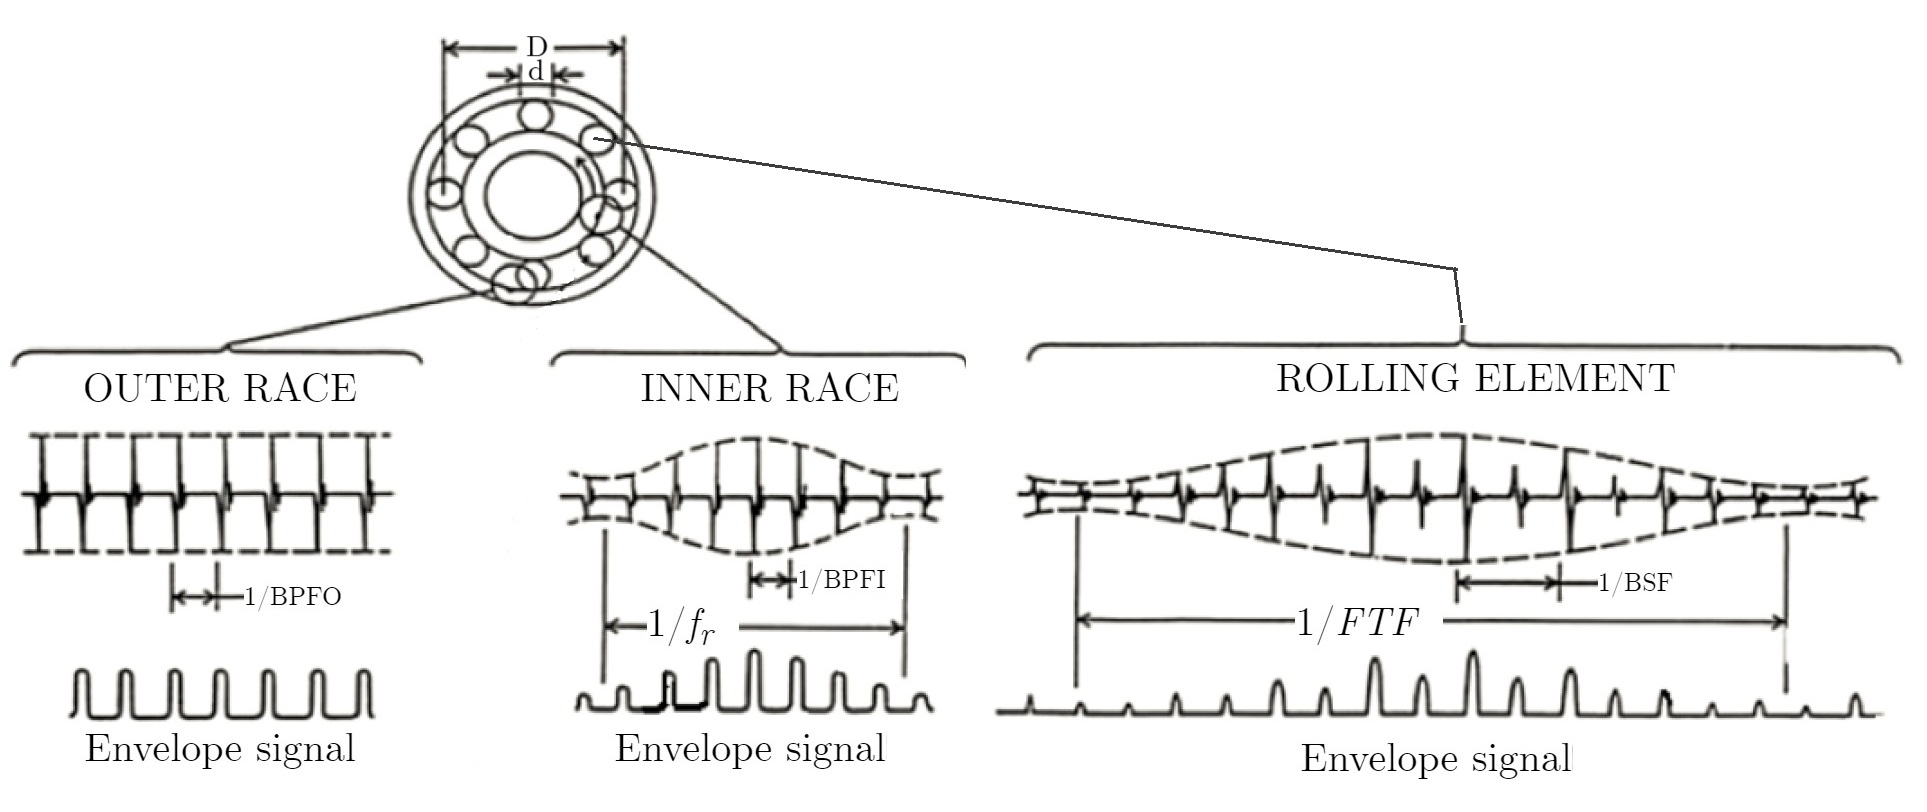
\includegraphics[width=\textwidth]{images/StateArt/bearing.jpg}
    \caption{Typical bearing fault signals \cite{RollingSignature}}
    \label{fig:bearing_faults}
\end{figure}

An automated method for bearing diagnosis has been developed by \cite{sawalhi2008semi}. The method is parametric and can be adapted to a large variety of cases. In the study, it has been tested on a helicopter gearbox, a high speed ($\approx 12000$rpm) test bench application and a low speed ($\approx 1800$rpm) radar tower. 

The automated procedure \cite{sawalhi2008semi} has been extended by a more recent study \cite{schlechtingen2019automated} where the authors applied a Cepstral Editing Procedure (\gls{cep}) based signal Pre-Whitening (\gls{pw}). The \gls{glo:frmwrk} has been tested on data collected from seventeen wind turbines. The procedure was successful in this case study, the preprocessing flow applied to the time-series, and the resulting spectral in which the \gls{bpfi} is exploited to detect the fault, are shown in \autoref{fig:turbine_faults}.

\begin{figure}
    \centering
    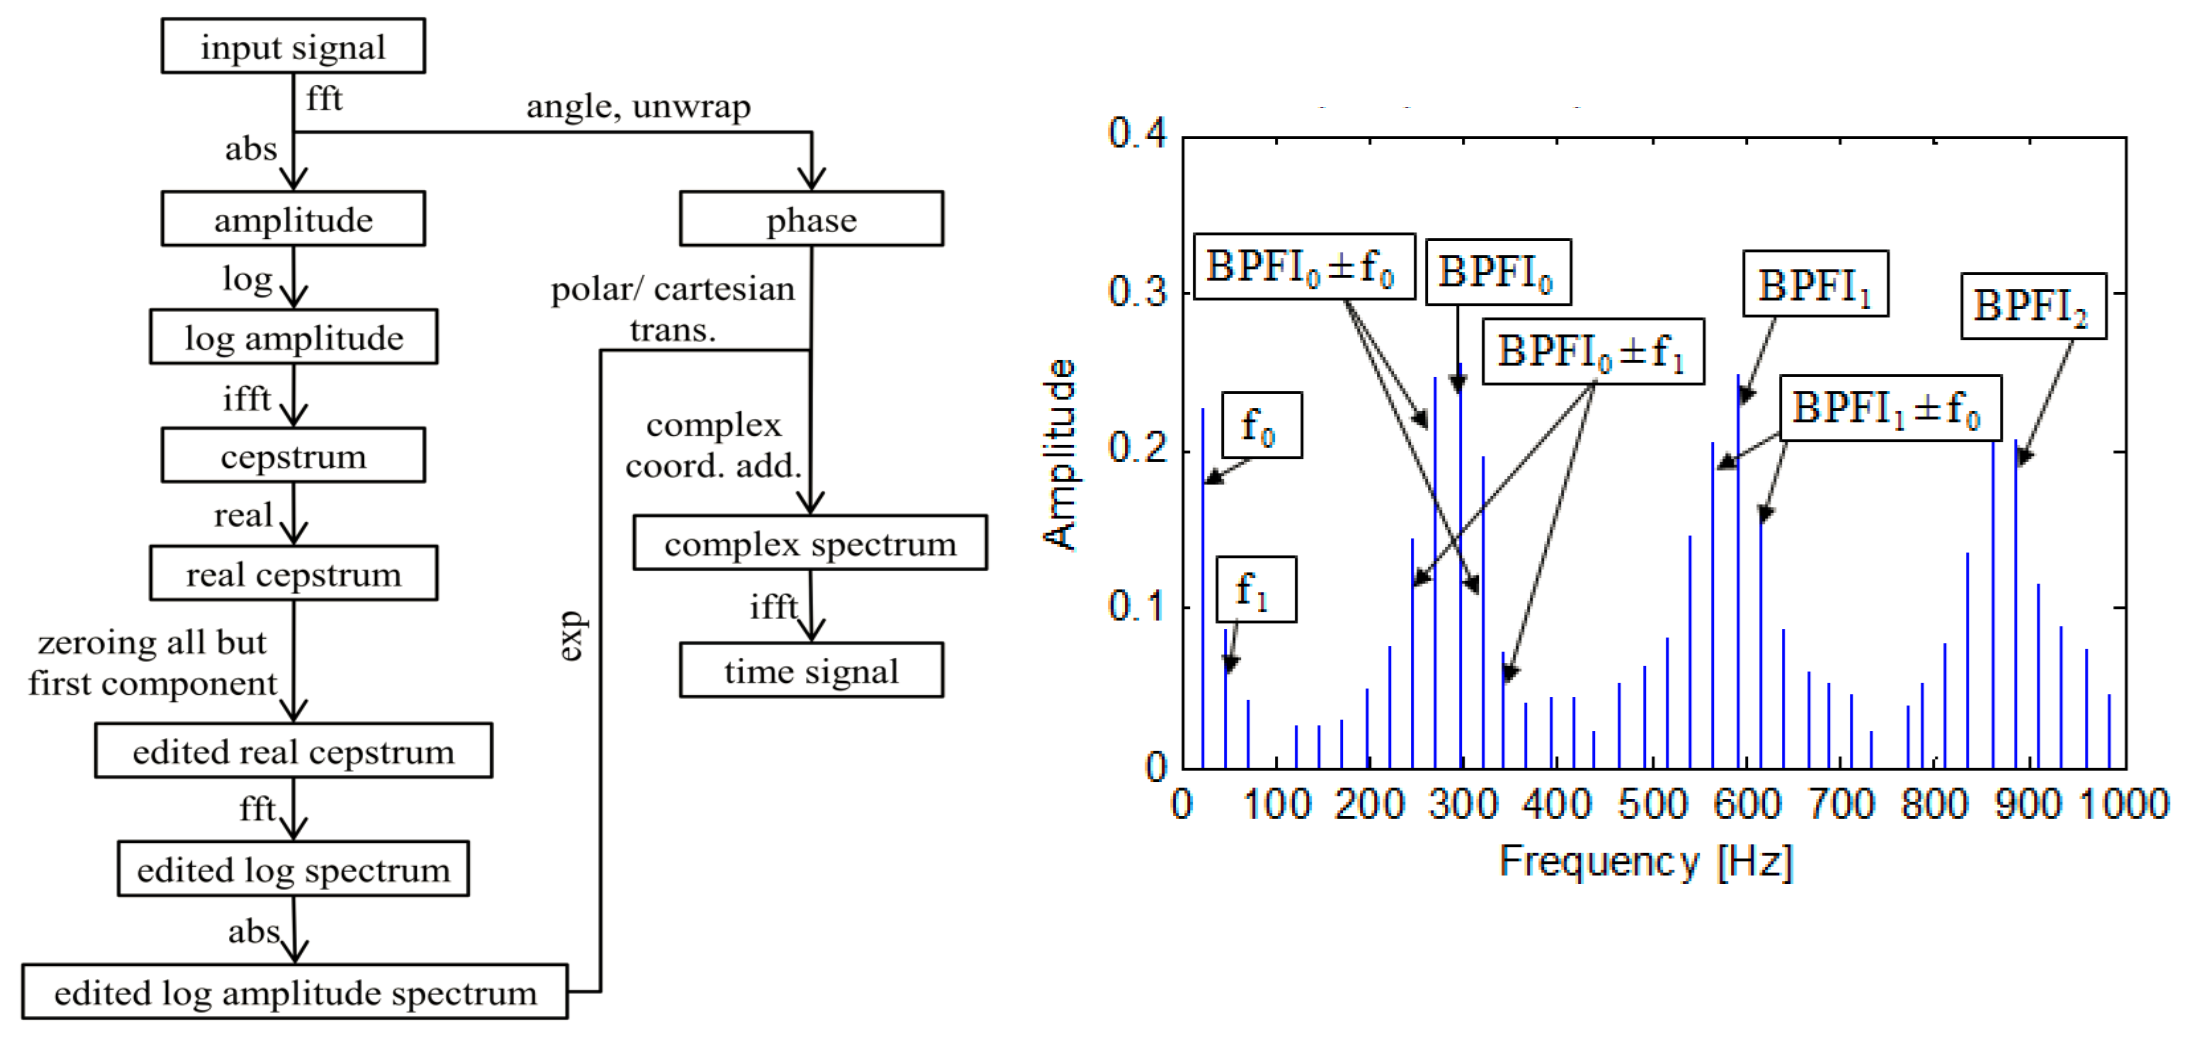
\includegraphics[width=\textwidth]{images/StateArt/spectrum.png}
    \caption{Preprocessing schematic and spectrum of a bearing fault signal \cite{schlechtingen2019automated}}
    \label{fig:turbine_faults}
\end{figure}

\subparagraph*{Novelty detection}
As anticipated, most of the time there is almost no precise knowledge about the physics of the system and data collections about faults are not available. In this case, \emph{novelty detection} (\gls{nd}) can be used. The task of detecting if a condition is \quoted{novel} can be seen as a classification problem with only one class (the data collected on the healthy system). The general idea is that if the one-class classifier is not able to classify a new observation as \quoted{healthy}, it means that the observation is \quoted{novel}.

Once the novelty detection algorithm is trained, it can be used to give an estimate of \quoted{how novel} the current behaviour of the system is. One of the major issues with \gls{nd} is to set the threshold value to decide if the observation is novel or not \cite{NoveltyReview}. This is because the value of the metric is hardly linkable to a physical property, and the span of the metric is not known a priori.

In \autoref{tab:novelTechniques}, the novelty detection techniques described in the comprehensive review \cite{NoveltyReview} are summarized. The review makes clear that in the field of \gls{nd}, both supervised and unsupervised techniques are used. It categorize the techniques into:
\begin{itemize}
    \item \textbf{Probabilistic} - involves a density estimation of the data;
    \item \textbf{Distance-based} - are the class of \gls{glo:clust}ing techniques used traditionally for classification;
    \item \textbf{Reconstruction-based} - use a regression model to reconstruct the data, then the error is used to detect the novelty;
    \item \textbf{Domain-based} - try to define a boundary that contains all the normal data;
    \item \textbf{Information-theoretic} - is based on the idea that novel data significantly alter the information content of the dataset.
\end{itemize}

{% \usepackage{tabularray}
\begin{longtblr}[
    caption = {State of the Art techniques for \gls{nd} \cite{NoveltyReview}},
    label = {tab:novelTechniques},
  ]{
    row{2} = {t},
    row{3} = {t},
    row{5} = {t},
    row{6} = {t},
    row{7} = {t},
    row{8} = {t},
    row{9} = {t},
    row{10} = {t},
    hline{1,11} = {-}{0.08em},
    hline{2} = {-}{},
  }
  \textbf{Model} & \textbf{Type}\\
  Mixture models & probabilistic, parametric\\
  State-space models & probabilistic, parametric\\
  Kernel density estimators & probabilistic\\
  Nearest neighbour & distance-based\\
  Clustering & distance-based\\
  Neural networs & reconstruction-based\\
  Subspace-based approaches~ & reconstruction-based\\
  Support vector descriptors & domain-based\\
  One-class support vectors & domain-based
  \end{longtblr}}

The first two terminologies are adopted also in the technical review of \gls{nd} methods \cite{NoveltyTech}. This study also categorizes the pattern to be identified in the following classes:
\begin{itemize}
    \item \textbf{Point pattern} - are single instances that are anomalous \gls{wrt} the rest of the data;
    \item \textbf{Contextual patter} - are anomalous \gls{wrt} a specific context;
    \item \textbf{Collective pattern} - is a collection of data instances that are anomalous if considered together.
\end{itemize}

The three distinct concepts are illustrated in \autoref{fig:pattern_types}.

The task of detecting the novelty is often associated with the task of predicting the \gls{glo:rul} (\gls{rul}) before the fault becomes fatal for the component.

\begin{figure}
    \centering
    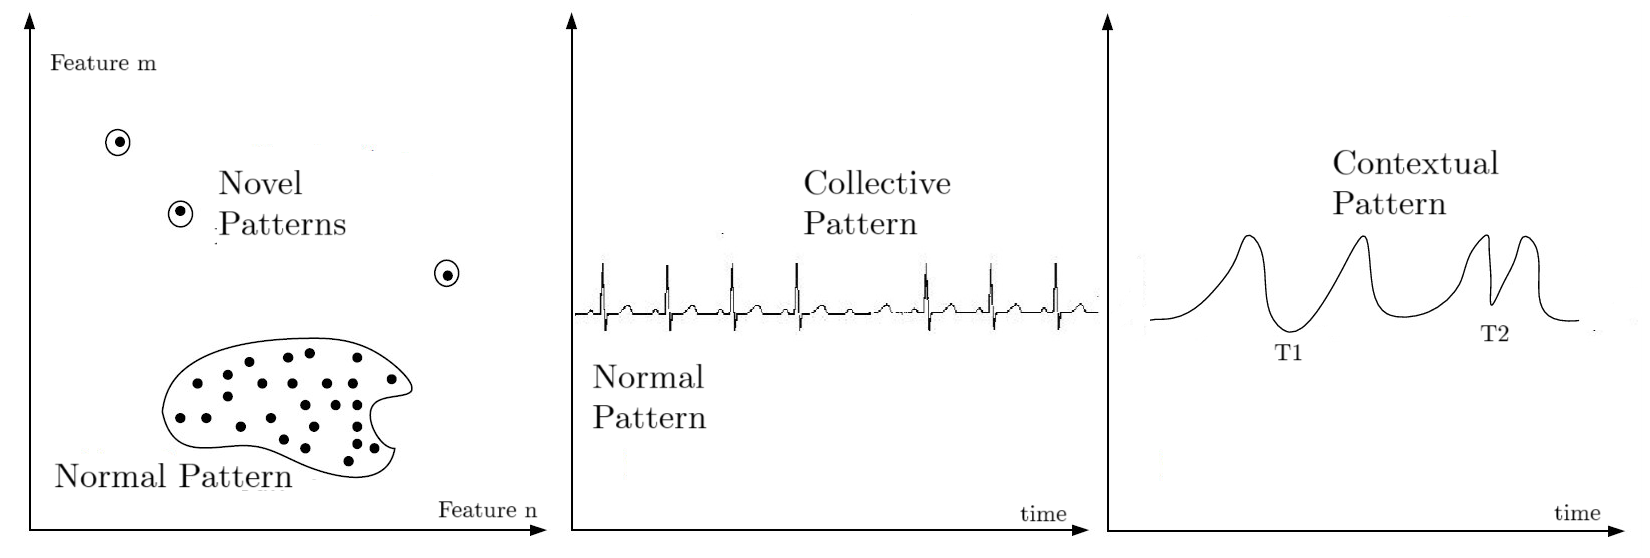
\includegraphics[width=\textwidth]{images/StateArt/patterns.png}
    \caption{Types of patterns \cite{NoveltyTech}}
    \label{fig:pattern_types}
\end{figure}

A novel \gls{glo:frmwrk} for performing \gls{nd}, \gls{fd} and \gls{rul} predictions has been proposed by researchers at PIC4SeR\footnote{\url{https://pic4ser.polito.it/}} \cite{Umberto}. It is based on several autonomous \gls{glo:agent}s working together on a database.  The authors aimed to perform \gls{pdm} in a scenario in which there is no physical knowledge and no prior data collections about the maintained system. The \gls{glo:frmwrk} is meant to be set in a \emph{training phase} on a new machine, to collect the \emph{normal} data and train the \gls{ml} model. After that, it will continuously work in \emph{testing mode}: the \gls{glo:frmwrk} will compute a prediction error on the current data that is used as a novelty metric.

The \gls{glo:feature}s are pre-processed using a windowing function and a cumulative absolute sum. Three regression models are used to perform \gls{nd} and \gls{fd}: a Linear Regressor \gls{lr}, a Decision Tree (\gls{dt}) and a Random Forest (\gls{rf}). The user of the \gls{glo:frmwrk} can decide which regressor to use in each specific case. 

The model can be retrained after a novelty has been detected, to update the model with the new data. Even if the \gls{glo:frmwrk} is meant to be trained on a new machine, it can be used also on a machine that has been in service for years: the faults already present will be part of the training database, but the predictions will still be useful because of the tendency of the faults to worsen over time.

The \gls{rul} predictions are made by averaging the prediction error in two intervals and then performing a linear regression on the two points. 

This \gls{glo:frmwrk} has been successfully tested on:  
\begin{itemize}
    \item a synthetic dataset that the authors created to emulate a bearing fault (using the definitions of the 4 typical faults \cite{RollingSignature}).
    \item a real dataset of bearing faults provided by the Center for Intelligent Maintenance Systems \cite{IMSpaper}
    \item a laboratory test on spring probes
\end{itemize}

In the first two cases, the \gls{glo:frmwrk} was able to detect the novelty and predict the \gls{rul}, in the laboratory test, it was able to recognise the new data as \emph{healthy} because the probes were not yet damaged. The graphical results of one test on real-world data are shown in \autoref{fig:umbertoresult}.

\begin{figure}
    \centering
    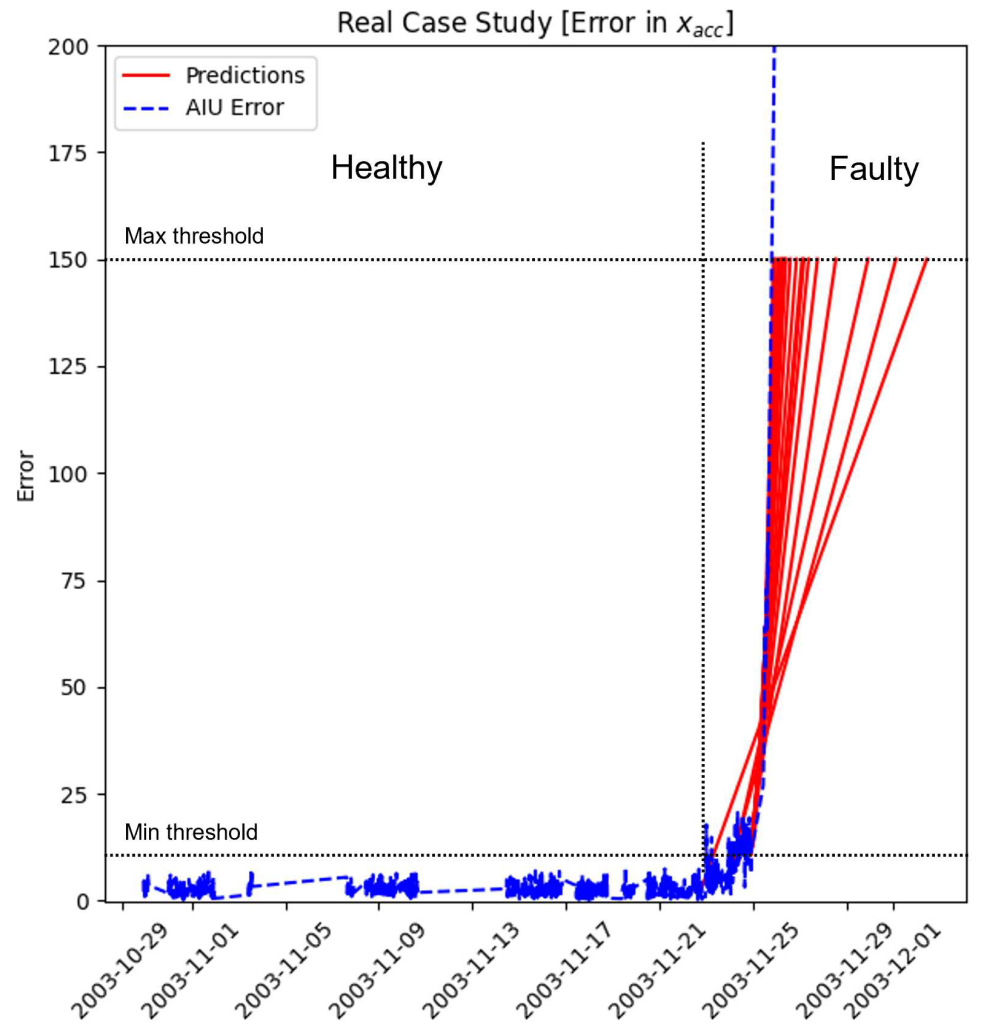
\includegraphics[width=0.6\textwidth]{images/IMS/UmbertoResults.png}
    \caption{Results provided by \cite{Umberto} for the test $\text{n}^\circ$1 of \gls{ims} dataset.}
    \label{fig:umbertoresult}
\end{figure}


\paragraph*{Clustering}
The most common unsupervised task is \gls{glo:clust}ing. In recent years, the volume of data collected in a typical factory has increased dramatically. Clustering is a collection of tools to extract information from huge amounts of unlabeled data. 

These algorithms can be divided into: \emph{partitioning-based} where the task is to define the boundaries between the \gls{glo:clust}s; \emph{hierarchical-based} that shows the relation between each pair of \gls{glo:clust}s depending on the medium of similarity or dissimilarity; \emph{density-based} that describes the \gls{glo:clust}s as a dense region of data points separated by low-density regions; \emph{grid-based} that apply the transformation of the \gls{glo:feature} space into a grid before proceeding with the \gls{glo:clust}ing and \emph{model-based} that use a statistical or deep-learning model to describe the data.

Recently, the survey \cite{Abla2019survey} provided a comprehensive overview of the most common \gls{glo:clust}ing algorithms used in an industrial context, with reference studies. The comparison of the study is reported in \autoref{tab:clustcomparison}.

{\small% \usepackage{color}
% \usepackage{tabularray}
\begin{longtblr}[
    caption = {Clustering algorithms comparison \cite{Abla2019survey}. $n$ = number of samples, $k$ = number of clusters, $d$ = number of features.},
    label = {tab:clustcomparison},
  ]{
    cell{2}{1} = {t},
    cell{2}{2} = {t},
    cell{3}{1} = {t},
    cell{3}{2} = {t},
    cell{5}{1} = {t},
    cell{5}{2} = {t},
    cell{6}{1} = {t},
    cell{6}{2} = {t},
    cell{7}{1} = {t},
    cell{7}{2} = {t},
    cell{8}{1} = {t},
    cell{8}{2} = {t},
    cell{9}{1} = {t},
    cell{9}{2} = {t},
    cell{10}{1} = {t},
    cell{10}{2} = {t},
    hline{1,23} = {-}{0.08em},
    hline{2} = {-}{},
  }
  \textbf{Algorithm} & \textbf{Volume} & {\textbf{High}\\\textbf{dim.}} & {\textbf{Cluster}\\\textbf{shape}} & \textbf{Complexity} & \textbf{n. param.}\\
  K-means & any & no & non-convex & $\mathcal{O}(nkd)$ & 1\\
  K-modes & large & yes & non-convex & $\mathcal{O}(n)$ & 1\\
  K-medioids & small & yes & non-convex & $\mathcal{O}(n^2dt)$ & 1\\
  PAM & small & no & non-convex & $\mathcal{O}(k(n-k)^2)$ & 1\\
  CLARA & large & no & non-convex & $\mathcal{O}(k(40+k)^2+$&1\\
  &&&&$+k(n-k))$ & \\
  Ward & any & no & non-convex & $\mathcal{O}(n)$ & 1\\
  BIRCH & large & no & non-convex & $\mathcal{O}(n)$ & 2\\
  CURE & large & yes & any & $\mathcal{O}(n^2\log n)$ & 2\\
  ROCK & large & no & any & $\mathcal{O}(n^2+n^2 \log n)$ & 1\\
  Chamelon & large & yes & any & $\mathcal{O}(n^2)$ & 3\\
  \gls{dbscan} & large & no & any & $\mathcal{O}(n \log n)$ & 2\\
  OPTICS & large & no & any & $\mathcal{O}(n \log n)$ & 2\\
  DENCLUE & large & yes & any & $\mathcal{O}(D)$ & 2\\
  Wavecluster & large & no & any & $\mathcal{O}(n)$ & 3\\
  STING & large & no & any & $\mathcal{O}(k)$ & 1\\
  CLIQUE & large & yes & any & $\mathcal{O}(ck+mk)$ & 2\\
  OPTGRID & large & yes & any & $\mathcal{O}(nd \log n)$ & 3\\
  \gls{em} & large & yes & non-convex & $\mathcal{O}(knp)$ & 3\\
  COBWEB & small & no & non-convex & $\mathcal{O}(n^2)$ & 1\\
  \gls{som} & small & yes & non-convex & $\mathcal{O}(n^2m)$ & 2\\
  \end{longtblr}}}
\mask{\chapter{Machine Learning}
\label{ch:MachineLearning}

Before diving into the description of the unsupervised algorithms used for the development of this thesis work presented in \autoref{ch:Unsupervised}, this chapter aims to be an introduction of \emph{Machine Learning} (\gls{ml}) in general.

An early but useful definition of Machine Learning was given by Arthur Samuel in 1959: \quoted{\emph{Machine learning is the field of study that gives computers the ability to learn without being explicitly programmed.}} A more recent definition is the following, from Tom Mitchell: \quoted{\emph{A computer program is said to learn from experience E with respect to some task T and some performance measure P, if its performance on T, as measured by P, improves with experience E.}} \citepage{hands-on-geron2022}{4}

So, in general, the ingredients of \gls{ml} are:
\begin{itemize}
    \item some data linked to some task
    \item a task to be performed
    \item an algorithm that learns how to perform the task on specific data
\end{itemize}

The data are usually preprocessed before giving them to the algorithm. The processed data are called \emph{features}. This is a generic term that refers to the information content of the data.
For example, if the data are recordings of temperatures over time, the features could be the mean, the standard deviation, the minimum, and the maximum of the temperature or, in some cases if the algorithm is able to learn directly from them, the raw data themself.

The tasks can be divided into main categories:
\begin{itemize}
    \item regression: the algorithm is trained to measure the relation between the value of output variables and corresponding values of other input variables;
    \item classification: the algorithm is trained to assign a label to a new instance, based on the training dataset of labelled instances;
    \item clustering: the algorithm is trained to group similar instances into clusters.
    \item anomaly detection: the algorithm is trained to identify instances that are different from known previous instances.
\end{itemize}

\section{Regression}
\label{sec:Regression}


\subsection{Least Squares}
\label{subsec:LS}

Let's consider a set of $m$ observations of a variable $y \in \mathbb{R}^{n_y}$ (output features) that depends on a variable $x \in \mathbb{R}^{n_x}$ (input features) and a set of $n_f \cdot n_y$ parameters $\theta \in \mathbb{R}^{n_f \times n_y}$.

Suppose to know that the output features are linked to the input features with $n_f$ functions linear in the parameters $\theta$, so that:
\begin{multline*}
    \begin{bmatrix}
        y_1 & y_2 & \dots & y_{n_y} 
    \end{bmatrix}
    =\\
        \begin{bmatrix}
            f_1(x_1, \dots, x_{n_x}) & f_2(x_1, \dots, x_{n_x}) & \dots & f_{n_f}(x_1, \dots, x_{n_x}) \\
        \end{bmatrix}
        \cdot
        \begin{bmatrix}
            \theta_{1,1}  & \dots & \theta_{1,n_y} \\
            \theta_{2,1}  & \dots & \theta_{2,n_y} \\
            \vdots & \ddots & \vdots \\
            \theta_{n_f,1}  & \dots & \theta_{n_f,n_y} \\
        \end{bmatrix}
\end{multline*}

Where all the $f_i$ are any known functions, $y_i$ and $x_i$ are known data and $\theta_{i,j}$ are the parameters to be found.

Considering the $m$ observations, the previous equation can be extended as:

\begin{multline*}
    \begin{bmatrix}
        y_{1,1} & y_{1,2} & \dots & y_{1,n_y} \\
        y_{2,1} & y_{2,2} & \dots & y_{2,n_y} \\
        \vdots & \ddots & \vdots \\
        y_{m,1} & y_{m,2} & \dots & y_{m,n_y} \\
    \end{bmatrix}
    =\\
        \begin{bmatrix}
            f_1(x_{1,1}, \dots, x_{1,n_x}) & \dots & f_{n_f}(x_{1,1}, \dots, x_{1,n_x}) \\
            f_1(x_{2,1}, \dots, x_{2,n_x}) & \dots & f_{n_f}(x_{2,1}, \dots, x_{2,n_x}) \\
            \vdots  & \ddots & \vdots \\
            f_1(x_{m,1}, \dots, x_{m,n_x}) & \dots & f_{n_f}(x_{m,1}, \dots, x_{m,n_x}) \\
        \end{bmatrix}
        \cdot
        \begin{bmatrix}
            \theta_{1,1}  & \dots & \theta_{1,n_y} \\
            \theta_{2,1}  & \dots & \theta_{2,n_y} \\
            \vdots & \ddots & \vdots \\
            \theta_{n_f,1}  & \dots & \theta_{n_f,n_y} \\
        \end{bmatrix}
\end{multline*}


Rewriting the previous equation in a more compact form:

\begin{equation}
    \begin{bmatrix}
        \vect{y}_1 \\
        \vect{y}_2 \\
        \vdots \\
        \vect{y}_m \\
    \end{bmatrix}
    =
    \begin{bmatrix}
        f_1(\vect{x}_1) & f_2(\vect{x}_1) & \dots & f_{n_f}(\vect{x}_1) \\
        f_1(\vect{x}_2) & f_2(\vect{x}_2) & \dots & f_{n_f}(\vect{x}_2) \\
        \vdots & \ddots & \vdots \\
        f_1(\vect{x}_m) & f_2(\vect{x}_m) & \dots & f_{n_f}(\vect{x}_m) \\
    \end{bmatrix}
    \cdot
    \begin{bmatrix}
        \theta_{1,1}  & \dots & \theta_{1,n_y} \\
        \theta_{2,1}  & \dots & \theta_{2,n_y} \\
        \vdots & \ddots & \vdots \\
        \theta_{n_f,1}  & \dots & \theta_{n_f,n_y} \\
    \end{bmatrix}
\end{equation}

That, in the most compact form, becomes:

\begin{equation}
    \vect{Y} = \vect{\Phi}(\vect{X}) \cdot \vect{\Theta}
\end{equation}

In close form, there is a solution $\vect{\Theta_{LS}}$, for estimating the parameters that minimize the error between the estimated output $\vect{Y_{LS}} = \vect{\Phi(\vect{X})}\vect{\Theta_{LS}}$ and the real output $\vect{Y_{}}$, that is known. Let's see, in an intuitive way:
\begin{eqnarray}
    \vect{Y} &=& \vect{\Phi}(\vect{X}) \cdot \vect{\Theta_{LS}} \\
    \vect{\Phi}(\vect{X})^T\vect{Y} &=& \underbrace{\vect{\Phi}(\vect{X})^T\vect{\Phi}(\vect{X})}_{\text{square}}\cdot \vect{\Theta_{LS}}\\
    (\vect{\Phi}(\vect{X})^T\vect{\Phi}(\vect{X}))^{-1}\vect{\Phi}(\vect{X})^T\vect{Y} &=& \vect{\Theta_{LS}}\\
    \text{pinv}(\vect{\Phi}(\vect{X}))\vect{Y} &=& \vect{\Theta_{LS}} \label{eq:LS}
\end{eqnarray}

In fact, it is known that $\vect{\Theta_{LS}} = \text{pinv}(\vect{\Phi}(\vect{X}))\vect{Y}$ is the solution of the following minimization problem:

\begin{equation}
    \vect{\Theta_{LS}} = \argmin{\vect{\Theta} \in \mathbb{R}^{n_f \times n_y}}{\norm{\vect{Y}-\vect{\Phi}(\vect{X})\vect{\Theta}}_2^2}
\end{equation}

That is why this method is called \emph{Least Squares} (\gls{ls}). It is proven that if the data $\vect{Y}$ affected my white noise, and the data $\vect{X}$ are known precisely, the solution converges to the real parameters $\vect{\Theta}_{\text{true}}$ when the number of observations $m$ goes to infinity.
\begin{equation}
    \lim_{m \to \infty} \vect{\Theta_{LS}} = \vect{\Theta}_{\text{true}}
\end{equation}

Is this considered machine learning? Yes, even being just a simple implementation of linear algebra, once programmed in a computer, it qualifies as the (simplest) machine learning algorithm because fitting new data does not require any human intervention. Let's see an example. Suppose to have 400 data points, shown in \autoref{fig:LinearRegressiondData}, of the variable $x$, $y_1$ and $y_2$ sampled with noise, that we call Feature 1, Feature 2 and Feature 3, respectively. Suppose that it is known that the output features are linked to the input feature with a linear combination of the functions $e^x$, $x^3$, $\cos(x)$, $\sin(x)$ and $\cos^3(x)$, but the parameters $\theta$ are unknown:

\begin{eqnarray}
    y_1 &=& \theta_{1,1} e^x + \theta_{2,1} x^3 + \theta_{3,1} \cos(x) + \theta_{4,1} \sin(x) + \theta_{5,1} \cos^3(x) \\
    y_2 &=& \theta_{1,2} e^x + \theta_{2,2} x^3 + \theta_{3,2} \cos(x) + \theta_{4,2} \sin(x) + \theta_{5,2} \cos^3(x)
\end{eqnarray}

\begin{figure}
    \centering
    \begin{subfigure}{0.49\textwidth}  % <----
        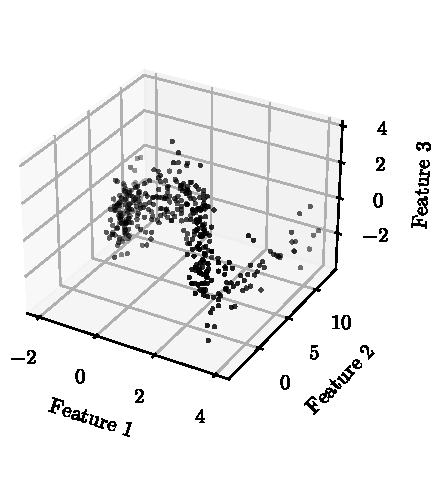
\includegraphics[width=\textwidth]{images/MachineLearning/LinearRegressiondData.pdf}
        \caption{400 data points}
        \label{fig:LinearRegressiondData}
    \end{subfigure}
    \begin{subfigure}{0.49\textwidth}  % <----
        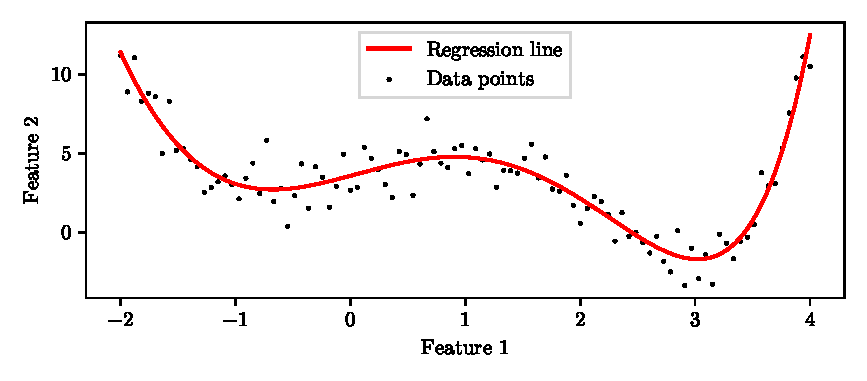
\includegraphics[width=\textwidth]{images/MachineLearning/LinearRegression.pdf}
        \caption{data points and the fitted curve}
        \label{fig:LinearRegression}
    \end{subfigure}
    \caption{Least square regression example}
\end{figure}

rearranging in matrix form: 
\begin{equation}
    \underbrace{\begin{bmatrix}
        y_{1,1} & y_{1,2} \\
        y_{2,1} & y_{2,2} \\
        \vdots & \vdots \\
        y_{m,1} & y_{m,2} \\
    \end{bmatrix}}_{\vect{Y}}
    =
    \underbrace{\begin{bmatrix}
        e^{x_1} & x_1^3 & \cos(x_1) & \sin(x_1) & \cos^3(x_1) \\
        e^{x_2} & x_2^3 & \cos(x_2) & \sin(x_2) & \cos^3(x_2) \\
        \vdots & \vdots & \vdots & \vdots & \vdots \\
        e^{x_m} & x_m^3 & \cos(x_m) & \sin(x_m) & \cos^3(x_m) \\
    \end{bmatrix}}_{\vect{\Phi}(\vect{X})}
    \cdot
    \underbrace{\begin{bmatrix}
        \theta_{1,1}  & \theta_{1,2} \\
        \theta_{2,1}  & \theta_{2,2} \\
        \theta_{3,1}  & \theta_{3,2} \\
        \theta_{4,1}  & \theta_{4,2} \\
        \theta_{5,1}  & \theta_{5,2} \\
    \end{bmatrix}}_{\vect{\Theta}}
\end{equation}

applying the \gls{ls} solution from \autoref{eq:LS}, we obtain:
\begin{equation*}
    \vect{\Theta_{LS}} = \text{pinv}(\vect{\Phi}(\vect{X}))\vect{Y} = 
    \begin{bmatrix}
        +1.997 & -0.004 \\
        -1.498 & +0.003 \\
        +1.332 & -0.018 \\
        -0.005 &  +0.999 \\
        -0.032 & +1.035 
    \end{bmatrix}
\end{equation*}

that is quite close to the real parameters used to generate the data:
\begin{equation*}
    \vect{\Theta}_{\text{true}} = 
    \begin{bmatrix}
        +2.0 & +0 \\
        -1.5 & +0 \\
        +1.3 & +0 \\
        +0.0 & +1 \\
        +0.0 & +1 
    \end{bmatrix}
\end{equation*}

Using the estimated parameters, it is possible to estimate the output features for new input features, the regression line is shown in \autoref{fig:LinearRegression}.

\subsubsection{Applicability}
This is an elegant closed-form solution for a regression problem, however, it has some limitations:
\begin{itemize}
    \item if the noise is not white, or it is present also in the input features, the solution is not guaranteed to converge to the real parameters;
    \item if there are nonlinearities in the parameters (for example $\sin(\theta_{1,1}x)$), the solution is not applicable;
\end{itemize}

\subsection{Gradient Descent \gls{gd}}
To overcome these limitations, another way to estimate the parameters is to use an iterative algorithm that minimizes a cost function over the parameters space. The iterations aim to update the parameters in the direction of the steepest descent of the cost function. This can be done even with nonlinearities in the data, and even if the noise is not white, but has the drawback of the risk of getting stuck in a local minimum of the cost function, starting from a random initialization.
Another limitation is the fact that a learning rate $\eta$ has to be defined, that is a parameter that defines how much the parameters are updated at each iteration. If the learning rate is too small, the algorithm will take a lot of time to converge, if it is too large, the algorithm may overshoot the minimum and avoid convergence.

In the previous closed form solution (\autoref{subsec:LS}), the hypothesis function was linear in the parameters $\vect{Y} = \vect{\Phi}(\vect{X})\cdot\vect{\Theta}$, so we can call this prediction $\vect{\hat{y}} = \vect{h}_{\vect{\Theta}}(\vect{x})$.

The cost function to be minimized is usually defined as the mean squared error between the prediction and the real data:
\begin{equation}
    \text{MSE}(\vect{X}, h_{\vect{\Theta}}) = \frac{1}{m}\sum_{i=1}^{m}(\vect{\hat{y}}_i - \vect{y}_i)^2
\end{equation}


The gradient of the cost function, used by all gradient descent algorithms, is defined as:

\begin{equation}
\nabla_{\vect{\Theta}} \text{MSE}(\vect{X}, h_{\vect{\Theta}}) = 
\begin{bmatrix}
    \frac{\partial}{\partial \theta_1} \text{MSE}(\vect{X}, h_{\vect{\Theta}}) \\
    \frac{\partial}{\partial \theta_2} \text{MSE}(\vect{X}, h_{\vect{\Theta}}) \\
    \vdots \\
    \frac{\partial}{\partial \theta_{n_f\times n_y}} \text{MSE}(\vect{X}, h_{\vect{\Theta}}) \\
\end{bmatrix}
\end{equation}

The algorithm then updates the parameters at each iteration as:
\begin{equation}
    \vect{\Theta}^{(i+1)} = \vect{\Theta}^{(i)} - \eta \nabla_{\vect{\Theta}} \text{MSE}(\vect{X}, h_{\vect{\Theta}})
\end{equation}


\subsection{Stochastic Gradient Descent}
\label{subsec:SGD}
The \emph{Stochastic Gradient Descent} (\gls{sgd}) is a variant of the \gls{gd} algorithm that computes the gradient only on one instance at each iteration, instead of on the whole dataset. This makes the algorithm much faster, but the cost function will be much more noisy, and theta will not reach a steady value but instead will oscillate around the minimum. This has the advantage of being more robust to local minimum entrapment, but the disadvantage of never reaching the minimum. To overcome this, the learning rate $\eta$ can be reduced at each iteration, but this will slow down the convergence.

\begin{figure}
    \centering
    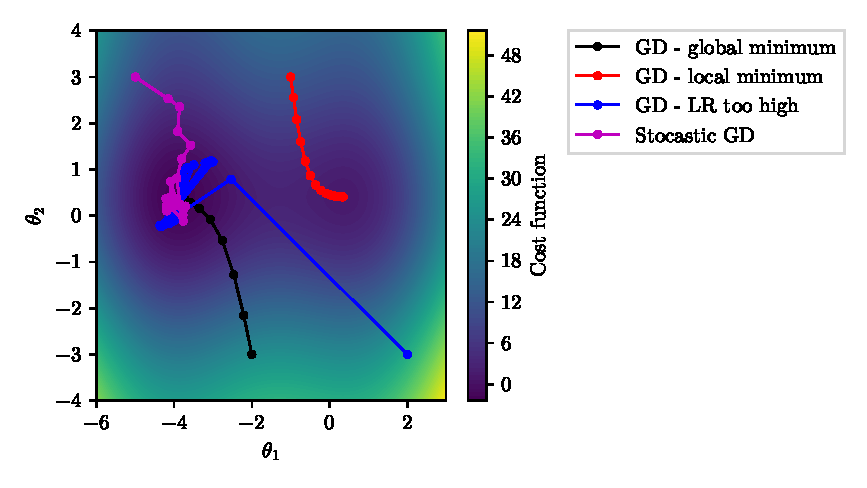
\includegraphics[width=\textwidth]{images/MachineLearning/GradientDescent.pdf}
    \caption{Gradient Descent comparison}
    \label{fig:SGD}
\end{figure}

In the \autoref{fig:SGD} it is visualized graphically what has been said about Gradient Descent.

\subsection{Avoid overfitting}
\label{subsec:overfitting}
The \gls{gd} algorithm is very powerful, but it can overfit the data. To avoid that, the problem of when to stop the iterations has to be addressed. A common way to do that is to split the dataset into a training set and a validation set. The training set is used to train the algorithm, and the validation set is used to evaluate the performance of the algorithm on new data. The training is stopped when the performance on the validation set starts to degrade, even if the performance on the training set is still improving. This is called \emph{early stopping}. In the \autoref{fig:overfitting} it is shown an example of early stopping using as metric the \emph{Root Mean Square Error} (RMSE), that is just the square root of MSE, on the validation set.

\begin{figure}
    \centering
    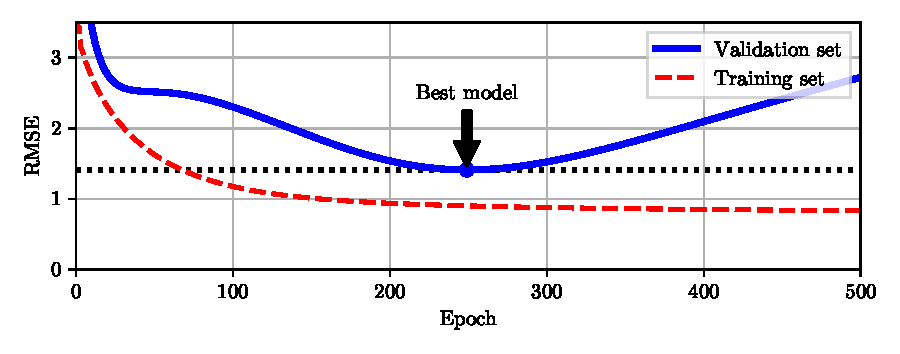
\includegraphics[width=\textwidth]{images/MachineLearning/EarlyStopping.pdf}
    \caption{Overfitting example \citepage{hands-on-geron2022}{162}}
    \label{fig:overfitting}
\end{figure}

\section{Classification}
\label{sec:Classification}
Another common task in \gls{ml} is classification. In this case, the algorithm is trained to assign a label to a new instance, based on the training dataset of labelled instances. Naively, it aims to define a set of rules that divide the space of the input features in regions, each one associated with a label. The two main approaches are \emph{hard} and \emph{soft} classification. In the former, the algorithm is trained to assign a single label to each instance, while in the latter, the algorithm is trained to output a probability for each label, and the label with the highest probability is assigned to the instance.

Classification is a \emph{supervised} learning task because the training dataset is labelled. The labels can be provided by a human or can be generated by another algorithm. Some classification algorithms are available also in the unsupervised version, where the labels are not provided, and the task is usually novelty detection.

\subsection{Support Vector Machines \gls{svm}}
\label{subsec:svm}
Support Vector Machines are simple but powerful classification algorithms that can be used both for hard and soft classification, with medium size datasets. They are based on the idea of finding the hyperplane that best divides the space of the input features into two regions, each one associated with a label.

The main drawback is that, natively, they can only be used for binary classification (two classes), but there are some extensions that allow to use of them for multiclass classification. Furthermore, as will be explained in \autoref{sec:OneClassSupportVectorMachine}, they can be used also for novelty detection (one class). Another limitation is that, being a linear classifier, they can only be used for linearly separable data, but using the \emph{kernel trick}, they can be used also for nonlinearly separable data.

\subsubsection{Linear \gls{svm}}
\label{subsubsec:LinearSVM}

\begin{figure}
    \centering
    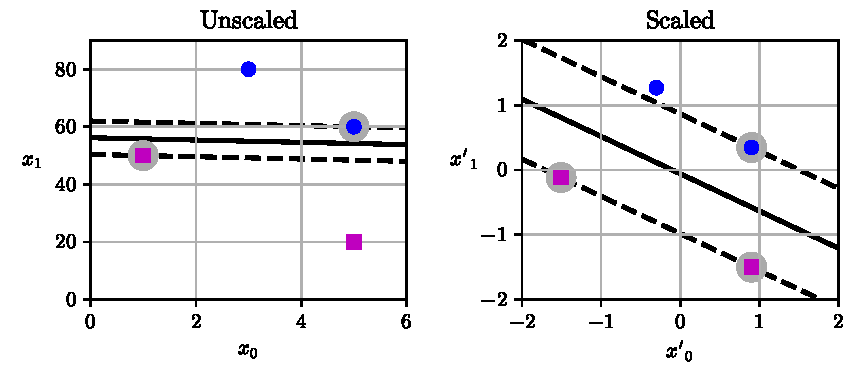
\includegraphics[width=\textwidth]{images/MachineLearning/LinearSVM.pdf}
    \caption{Linear SVM example \citepage{hands-on-geron2022}{176}}
    \label{fig:LinearSVM}
\end{figure}

Looking at \autoref{fig:LinearSVM}, it is possible to visualize what the algorithm does: it finds the plane that separates one class from the other, and vice-versa for the second class. In other words, it finds the most distant parallel hyperplanes that separate the two classes. As evident from the figure, the distance between the hyperplanes (called \emph{margin}) is sensitive to the features scaling. The term \quoted{support} derives from the fact that only the instances that are on the margin, define (support) the two planes. Those instances are called \emph{support vectors}, and in the figure are highlighted with a grey circle.

\subsubsection{Noninear \gls{svm}}
\label{subsubsec:NoninearSVM}
As said before, the \gls{svm} algorithm can be used also for nonlinearly separable data, using the \emph{kernel trick}. The idea is to project the data into a higher dimensional space, where they are linearly separable, and then use the linear \gls{svm} algorithm. The projection is done using a \emph{kernel mapping}. 

Let's have a look at what is the function for classifying an instance $\vect{x}^{(i)}$:
\begin{equation}
    t^{(i)} = \begin{cases}
        -1 & \text{if } \vect{w}^T\vect{x}^{(i)} + b < 0 \\
        1 & \text{if } \vect{w}^T\vect{x}^{(i)} + b \geq 0 
    \end{cases}
\end{equation}

The model is trained to find the parameters $\vect{w}$ and $b$ that:
\begin{align}
    \label{eq:LinearSVM}
    \underset{\vect{w},b}{\text{minimize }} & \frac{1}{2}\vect{w}^T\vect{w} \\
    \text{subject to } & t^{(i)}(\vect{w}^T\vect{x}^{(i)} + b) \geq 1 \quad \forall i = 1, \dots, m
\end{align}

Since the objective function is convex, and the inequality constraints are differentiable and convex, the solution is the same as the solution of the dual problem \citepage{hands-on-geron2022}{188}:
\begin{align}
    \label{eq:LinearSVMdual}
    \underset{\vect{\alpha}}{\text{minimize }} & \frac{1}{2}\sum_{i=1}^{m}\sum_{j=1}^{m}\alpha^{(i)}\alpha^{(j)}t^{(i)}t^{(j)}\vect{x}^{(i)T}\vect{x}^{(j)} -\sum_{i=1}^{m}\alpha^{(i)}\\
    \text{subject to } & \alpha^{(i)} \geq 0 \quad \forall i = 1, \dots, m \quad \text{and} \quad \sum_{i=1}^{m}\alpha^{(i)}t^{(i)}=0
\end{align}

\paragraph{Kernel Trick}
Suppose needing to use a second-degree polynomial mapping, the mapping function is defined as:
\begin{equation}
    \phi(\vect{x}) = \phi(\begin{bmatrix}
        x_1 \\
        x_2 \\
    \end{bmatrix}) = \begin{bmatrix}
        x_1^2 \\
        \sqrt{2}x_1x_2 \\
        x_2^2 \\
    \end{bmatrix}
\end{equation}

Transforming two vectors $\vect{a}$ and $\vect{b}$ with the mapping function, to be inserted in \autoref{eq:LinearSVMdual}:
\begin{equation}
    \phi(\vect{a})^T\phi(\vect{b}) = \begin{bmatrix}
        a_1^2 \\
        \sqrt{2}a_1a_2 \\
        a_2^2 \\
    \end{bmatrix}^T
    \begin{bmatrix}
        b_1^2 \\
        \sqrt{2}b_1b_2 \\
        b_2^2 \\
    \end{bmatrix} = a_1^2b_1^2 + 2a_1b_1a_2b_2 + a_2^2b_2^2 = (\vect{a}^T\vect{b})^2
\end{equation}

So, transforming with a polynomial mapping of degree $d$, does not require computing the mapping function, but just computing the dot product of the two vectors and elevating it to the degree $d$, in the dual problem. There also are other kinds of kernels, resumed in the following:
\begin{align*}
    \text{Linear: } & K(\vect{a}, \vect{b}) = \vect{a}^T\vect{b} \\
    \text{Polynomial: } & K(\vect{a}, \vect{b}) = (\gamma\vect{a}^T\vect{b} + r)^d \\
    \text{Gaussian RBF: } & K(\vect{a}, \vect{b}) = \exp(-\gamma\norm{\vect{a}-\vect{b}}^2) \\
    \text{Sigmoid: } & K(\vect{a}, \vect{b}) = \tanh(\gamma\vect{a}^T\vect{b} + r)
\end{align*}

\begin{figure}
    \centering
    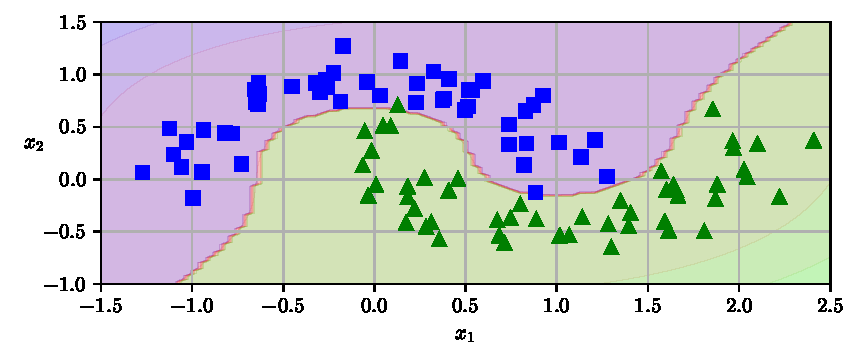
\includegraphics{images/MachineLearning/KernelTrick.pdf}
    \caption{Kernel Trick example \citepage{hands-on-geron2022}{180}}
    \label{fig:KernelTrick}
\end{figure}

The \autoref{fig:KernelTrick} shows an example of \gls{svm} classification of data that are not linearly separable.

This topic seems unrelated to the scope of this thesis, but in \autoref{sec:OneClassSupportVectorMachine} we will see how to use the \gls{svm} algorithm for novelty detection, as a one-class classifier.


\subsection{Decision Trees \gls{dt}}
\label{subsec:dt}

\begin{figure}
    \centering
    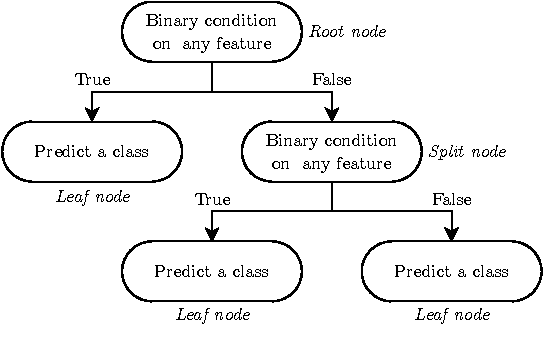
\includegraphics[scale = 1]{images/MachineLearning/DT_structure.pdf}
    \caption{Decision Tree structure}
    \label{fig:DecisionTree}
\end{figure}

Decision Trees are very powerful classification algorithms that can also be used for regression, thinking of feature values as classes. The classification process is based on a tree structure, where each sample starts from the root node, and is filtered through a bunch of \emph{if - then} statements until it reaches a leaf node, that outputs the predicted class. In \autoref{fig:DecisionTree}, it is illustrated the structure of a very simple binary tree with only a split node and three leaf nodes.

\paragraph*{Gini impurity}
The classification algorithm is hence very simple, the \gls{ml} part is the training process. Let's consider a leaf node, and imagine processing all the training samples through the tree. Ideally, all the samples that reach the leaf node (and any other leaf node) should have the same class. This is possible, but a tree that does that is most likely very overfitted to the training dataset and will not perform well on future data. Anyway, the aim of training is to obtain a tree close enough to the ideal one, without overfitting. To do that, there exists a metric called \emph{Gini impurity} that assumes a value of zero if the leaf node is pure (all the samples that reach it have the same class), or a positive value $\in (0,0.5]$ that measures how different the classes in the node are, 0.5 being the maximum value that means that all the classes are present in the node with equal frequency. The mathematical definition is the following:
\begin{equation}
    G_i = 1 - \sum_{k=1}^{n}p_{i,k}^2
\end{equation}
where $p_{i,k}$ is the ratio of class $k$ instances among the training instances in the $i^{th}$ node.

Then the training procedure tries to grow a tree defining the binary conditions that minimizes the weighted average of the Gini impurity of the two child nodes, so the cost function is:
\begin{equation}
    J(k, t_k) = \frac{m_{\text{left}}}{m}G_{\text{left}} + \frac{m_{\text{right}}}{m}G_{\text{right}}
\end{equation}
where $k$ is the feature index, $t_k$ is the threshold value, $m_{\text{left}}$ and $m_{\text{right}}$ are the number of instances in the left and right child nodes, and $G_{\text{left}}$ and $G_{\text{right}}$ are the Gini impurity of the left and right child nodes.

A common way for minimization of the cost function is to use the \emph{Classification and Regression Tree} (\gls{cart}) algorithm, which is a greedy algorithm that searches for the optimal split at each node, but not for the global optimal tree. The algorithm complexity is $\mathcal{O}(n \times m \log_2(m))$.

\paragraph{Entropy}
Another metric that can be used instead of Gini impurity inside the same cost function is the \emph{entropy} of the node, which is defined as:
\begin{equation}
    H_i = - \sum_{k=1}^{n}p_{i,k}\log_2(p_{i,k})
\end{equation}

This renders trees very similar to the ones obtained using Gini impurity, but the entropy is slightly slower to compute, due to the logarithm. however, it tends to produce slightly more balanced trees \cite{raschka2013decisiontrees}.

\paragraph{Avoid overfitting}
To avoid overfitting the data, the \gls{cart} algorithm implementation in \texttt{sklearn} has some \gls{glo:hyperparameter}s that can be tuned:
\begin{itemize}
    \item \texttt{max\_depth}: the maximum depth of the tree;
    \item \texttt{min\_samples\_split}: the minimum number of samples a node must have before it can be split;
    \item \texttt{min\_samples\_leaf}: the minimum number of samples a leaf node must have;
    \item \texttt{max\_leaf\_nodes}: the maximum number of leaf nodes;
    \item \texttt{max\_features}: the maximum number of features that are evaluated for splitting at each node.
\end{itemize}
Increasing the \texttt{min} bound, or decreasing the \texttt{max} bound, will regularize the model, and reduce the risk of overfitting.
In \autoref{fig:DecisionTreeOverfitting} it is shown an example of overfitting, where the left plot shows the decision boundaries of a tree with no regularization, and the right plot shows the decision boundaries of a tree with regularization.

\begin{figure}
    \centering
    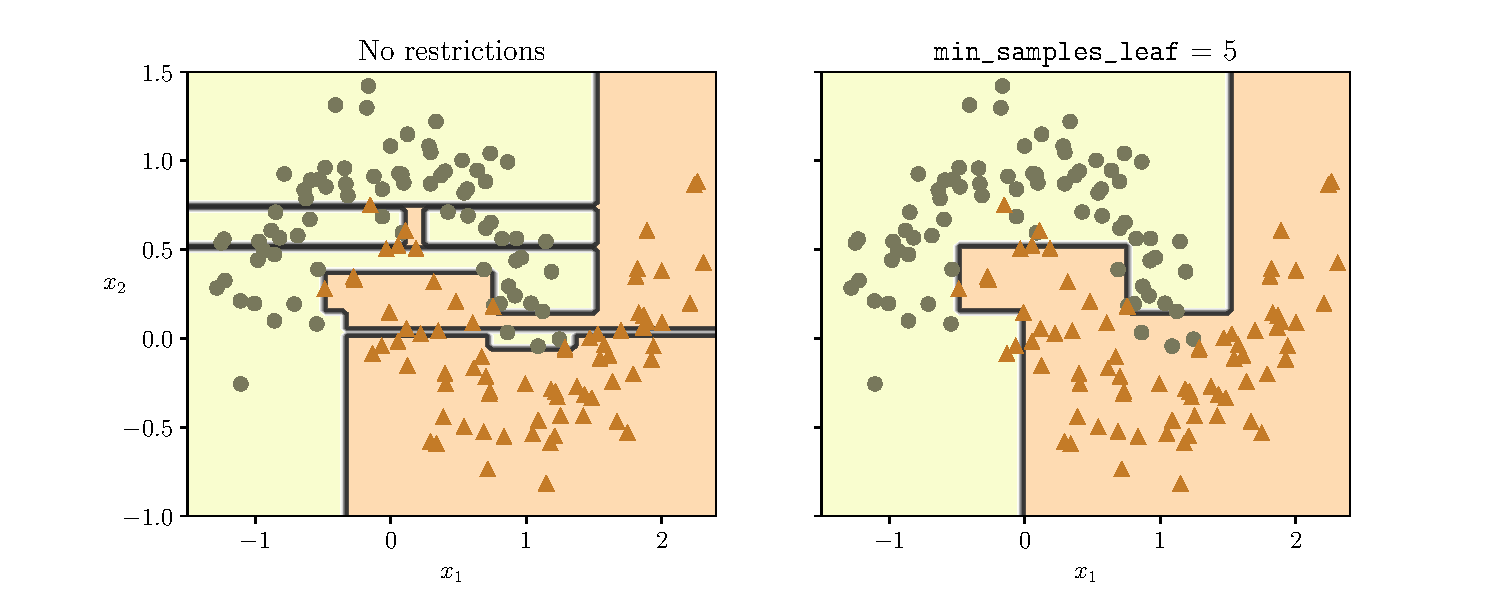
\includegraphics{images/MachineLearning/DecisionTreeOverfitting.pdf}
    \caption{Decision Tree overfitting example \citepage{hands-on-geron2022}{203}}
    \label{fig:DecisionTreeOverfitting}
\end{figure}

\paragraph{Regression}
As anticipated, the \gls{dt}s can also be used for regression, in this case, the cost function is the \gls{mse} of the predicted value in the leaf node:
\begin{equation}
    J(k, t_k) = \frac{m_{\text{left}}}{m}\text{MSE}_{\text{left}} + \frac{m_{\text{right}}}{m}\text{MSE}_{\text{right}}
\end{equation}

\paragraph{Advantages and limitations}
The main disadvantages of \gls{dt}s are that the classification procedure uses thresholds on the value of the features (cutting the hyperspace in orthogonal hyperplanes), so they are sensitive to axis orientation, and they are very sensitive to small variations in the training data. They are also very sensitive to the \gls{glo:hyperparameter}s, so a small variation in constraints leads to very different trees. The main advantages are that they are very fast to train, and the resulting model is very fast to make predictions, they are very easy to understand and visualize and they do not require any feature scaling or centring.

\subsection{Random Forests \gls{rf}}
\label{subsec:rf}
The high sensitivity of the \gls{dt}s to small variations in the training data, can be reduced using the \emph{Random Forests} (\gls{rf}) algorithm. The idea is to train a bunch of \gls{dt}s on different random subsets of the training data, and then to average their predictions. The subsets of the training set are usually picked randomly with replacement, this technique is called \emph{bagging} (short for \emph{bootstrap aggregating}). 

The benefits of using more threes on subsets of the training data are shown in the \autoref{fig:RandomForest}. The left plot shows the decision boundaries of a single \gls{dt}, and the right plot shows the decision boundaries of a \gls{rf} with 500 trees.

\begin{figure}
    \centering
    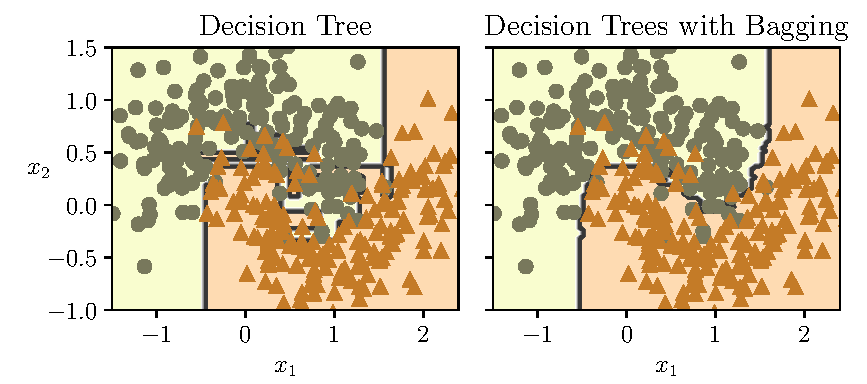
\includegraphics{images/MachineLearning/RandomForest.pdf}
    \caption{Random Forest example \citepage{hands-on-geron2022}{218}}
    \label{fig:RandomForest}
\end{figure}

Again, this topic seems unrelated to the scope of this thesis, but in \autoref{sec:IsolationForest} we will see how to use the \gls{rf} algorithm for novelty detection, exploiting the fact that outliers are usually more isolated (require more split nodes to be reached) than the normal instances.}
\mask{\chapter{Unsupervsed learning}
\label{ch:clustering}

\chapter{Clustering}
\label{ch:clustering}

\section{K-means algorithm}
\label{sec:kmeans}

Let's assume to have extrapolated $F$ features from each of our signals, to produce a set $\snapshot$ of $n$ snapshots $\snapshot_i, i \in [1,n], \snapshot_i \in \snapshot $ (every snapshot is a vector of features $\in \mathbb{R}^F$). The task is to define a set $\cluster$ of $k$ clusters ($k \leq n$) $\cluster_i, i \in [1,k], \cluster_i \in \cluster$ that minimize the squared sum of the distances between the snapshots and the centroids $\vect{c}_i$ of the clusters they belong to. This is equivalent to find the centroids that minimize the variance of the clusters themeself, so the problem can be formulated as in the \autoref{eq:kmeans_problem}.

\begin{equation}
  \argmin{\cluster}\sum_{i=1}^{k}\sum_{\snapshot_j \in \cluster_i} \norm{\snapshot_j - \vect{c}_i}^2 = \argmin{\cluster}\sum_{i=1}^{k}\abs{\cluster_i}\mathrm{Var}\cluster_i
\label{eq:kmeans_problem}
\end{equation}

Unfortunately, this problem is NP-hard, even for as little as $F=2$ features considered \cite{MAHAJAN201213}, so it is not possible to guarantee to find the global optimum in a reasonable time. 

Anyway, euristic clustering algorithms were already developed in the 1950s. The first appearence of the therm \quoted{K-means} was used in 1957 by MacQueen \cite{macqueen1967some}, and the algorithm settled to a \quoted{standard} version in 1982 \cite{Lloyd1982}.

Nowadays, the K-means algorithm is one of the most used clustering algorithms, and it is implemented in many libraries, such as \texttt{scikit-learn} for \texttt{Python}, and others for \texttt{C}, \texttt{R}, \texttt{MATLAB}, etc. However, the runtime performances vary widely depending on the implementation \cite{Kmeans-performances-Kriegel2017}. The problem of the algorithm returning a local minima instead of the global one is still present. Most implementation try to minimise the probability of returning this sub-optimal result running the algorithm multiple times with different initializations, and then selecting the best result.

\subsection{Training}

\begin{figure}[htbp]
  \centering
  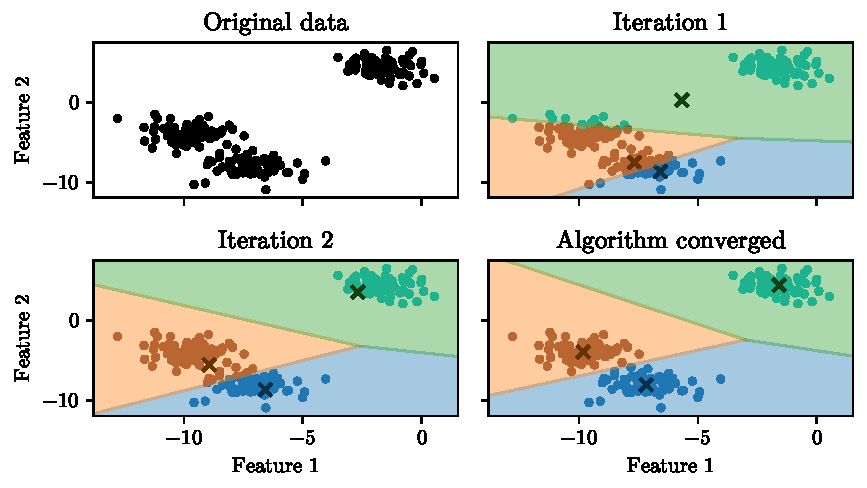
\includegraphics[width=\textwidth]{images/Kmeans_vornoi.pdf}
  \caption{K-means algorithm in the $2$-dimensional space}
  \label{fig:kmeans_vornoi}
\end{figure}

\paragraph*{K-means} The naive kmeans algorith consist in a series of iterions. First, the centroids $\vect{c}_i$ are initialized randomly, then the snapshots are assigned to the nearest centroid, and finally the centroids are updated as the mean of the snapshots assigned to them. These steps are repeated untill the position of the centroids does not change anymore, or a defined maximum number of iterations is reached. This naive algorithm is summarized in the following \autoref{alg:kmeans}.

\begin{algorithm}
  \caption{Training of the K-means model}
  \label{alg:kmeans}
  \begin{algorithmic}[1]
  \Function{K-means.train}{$\snapshot, k$}
  \LineComment{$\snapshot$ is the set of snapshots to be clustered}
  \LineComment{$k$ is the number of clusters to be obtained}
  \State $\vect{c}_i \gets \text{random initialization}, \forall i \in [1,k], \vect{c}_i \in \text{Domain of }\snapshot$
  \Repeat
  \LineComment{Every snapshot is assigned to the nearest centroid. Every centroid defines a cluster containing the assigned snapshots}
  \State $\cluster_i \gets \left\{ \snapshot_p : \norm{\snapshot_p - \vect{c}_i}^2 \leq  \norm{\snapshot_p - \vect{c}_j}^2  \forall j \in [1,k] \right\} \forall i \in [1,k] $
  \LineComment{The centroids are updated as the mean of their snapshots}
  \State $\vect{c}_i \gets \frac{1}{\abs{\cluster_i}}\sum_{\snapshot_j \in \cluster_i} \snapshot_j, \forall i \in [1,k]$, \Comment{$\abs{\cluster_i}$ is the cluster size}
  \Until{All the centroids do not change anymore, or max iterations reached}
  \State $r_i \gets \max{\norm{\snapshot_j-\vect{c}_i}, \, \forall \snapshot_j \in \cluster_i}, \, \forall i \in [1,k]$ 
  \State \Return $\mathcal{M}_{\text{\texttt{k-means}}}$  \Comment{The model contains the centroids $\vect{c}_i$, the radii ${r}_i$ of the clusters, and the labels of the snapshots}
  \EndFunction
  \end{algorithmic}
\end{algorithm}

As an example, we can consider $F=2$ features, and generate some test points shaped like tree separated clusters. In the \autoref{fig:kmeans_vornoi} are shown the original data, the first two iteration of the algorithm, and the final result. The K-means algorithm had $n=200$ snapshots, and $k=3$ clusters as input. The colors of the dots and the shaded areas represent the clusters, and the decision boundaries. The centroids are represented as black crosses. 
The decision boundaries are a vornoi tessellation of the space, and they are defined as the set of points that are equidistant from the centroids of two different clusters. The algorithm itself does not compute the boundaies, but it is useful to plot them for visualization purposes.

\paragraph*{K-means \texttt{++}}
\lipsum[1]

\subsection{Selecting the number of clusters}
It is important to notice that, even being an \emph{unsupervised} learning algorithm, the K-means algorithm needs to know the number of clusters $k$ in advance. There are some methods to decide what is the best number of clusters, but they usually need to perform more iterations of the algorithm with different values of $k$, and then compare the results. This task is hardly automatable so, during the training phase, the user has to decide the number of clusters to be used.

To compare the results of the different iterations, it is possible to use some metrics on the data and the centroids. The most common metrics are the \emph{inertia} and the \emph{silhouette score}, described in the following paragraphs.

\paragraph*{Inertia}
The inertia metric measure the total (sum) distance of each point belongigng to a cluster from the centroid of the cluster itself, as shown in the \autoref{eq:inertia}. This is called inertia because in the phisical sense it is the sub of the moment of inertia of each cluster if all the snapshots were considered as point masses (with unitary mass). This analogy is useful to understand that the lower the inertia, the more compact the clusters are.

Let's span $k \in [1,9]$ and plot the inertia of the clusters for each value of $k$, on the previous dataset. The result is shown in the \autoref{fig:kmeans_inertia}. As expected, the inertia decreases as the number of clusters increases. This is not a desirable behavior, if the aim is selecting the number of clusters, the best guess is to select (by eye or with some automatism) the Pareto optimal point (\acrshort{pof}) of the curve \cite{pareto}.

\begin{equation}
  \label{eq:inertia}
  I = \sum_{i=1}^{k}\sum_{\snapshot_j \in \cluster_i} \norm{\snapshot_j - \vect{c}_i}^2
\end{equation}

\begin{figure}
  \centering
  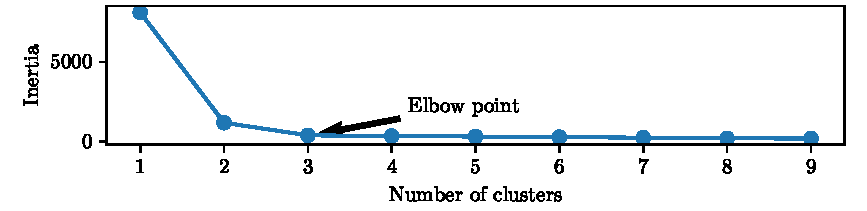
\includegraphics[width=\textwidth]{images/Kmeans_inertia.pdf}
  \caption{Inertia of the clusters for different values of $k$}
  \label{fig:kmeans_inertia}
\end{figure}




\subsection{Evaluation of a new instance}

At this point, with a model trained on the data, a generic $n$th new snapshot instance $\snapshot_n$ can be evaluated using the K-means algorithm.
From a geometric point of view, the snapshot $\snapshot_n$ is a point in the ${F}$-dimensional space, where ${F}$ is the number of features used to train the model.

For demonstration purposes, in this section, it is considered an example with ${F}=3$ features.

\begin{figure}[htbp]
  \centering
  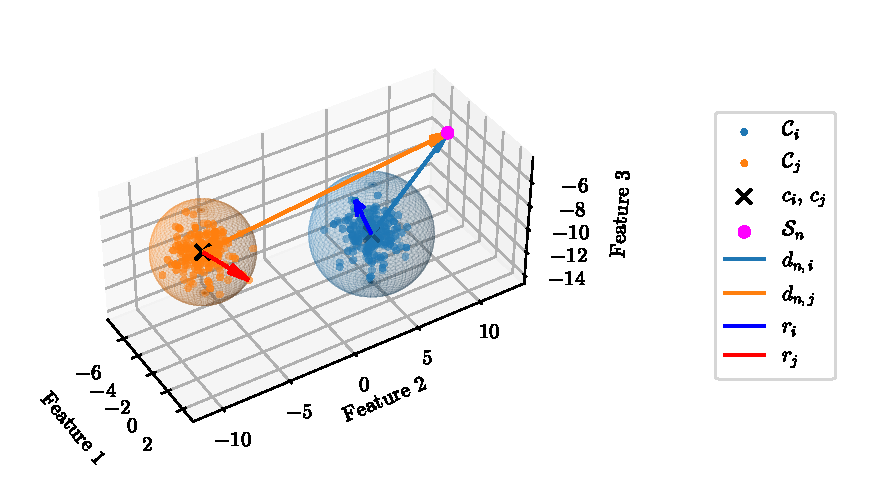
\includegraphics[width=\textwidth]{images/Spheres_2.pdf}
\caption{Cluster model in the $3$-dimensional space, with new snapshot $\snapshot_n$}
\label{fig:clust_spheres}
\end{figure}

In the \autoref{fig:clust_spheres}, the training data are represented in the $3$-dimensional space, where the axis are the features used to train the model. The K-means model has been ideally trained with an arbitrary number $k$ of clusters but, for display purposes, only two clusters  ($\cluster_i$ and $\cluster_j$) are plotted. 
\paragraph*{}
The entities shown in the \autoref{fig:clust_spheres} are:
\begin{itemize}
  \item $\vect{c}_{i(j)}$ is the centroid of the $i$th ($j$th) cluster;
  \item $\vect{r}_{i(j)}$ is the radius of the $i$th ($j$th) cluster, it is defined as the distance between the centroid $\vect{c}_{i(j)}$ and the farthest point belonging to the cluster itself;
  \item $\cluster_{i(j)}$ is the set of training snapshots belonging to the $i$th ($j$th) cluster, it has a centroid $\vect{c}_{i(j)}$ and a radius $\vect{r}_{i(j)}$;
  \item $\snapshot_n$ is the new snapshot to be evaluated;
  \item $\vect{d}_{n,i}$ is the vector between $\snapshot_n$ and $\vect{c}_i$;
  \item $\vect{d}_{n,j}$ is the vector between $\snapshot_n$ and $\vect{c}_j$;
  \item the semi-transparent spheres represent the cluster sizes, the radius of the spheres is the radius of the cluster itself, and the center is the centroid of the cluster;
\end{itemize}

\subsection{Assignation of the new instance to a cluster} 
The procedure for assigning the new snapshot $\snapshot_n$ to a cluster is quite simple, it is sufficient to compute the distance between $\snapshot_n$ and the centroids $\vect{c}_m$, $\forall m \in  [1, \dots , k]$. The distance is defined as the $l^2$-norm in the feature space, and can be computed using the \autoref{eq:clust_dist}, and assign $\snapshot_n$ to the cluster with the minimum distance.

\begin{equation}
  \label{eq:clust_dist}
  \vect{d}_{n,m} = ||\snapshot_{n,f} - \vect{c}_{m,f}||_2 = \sqrt{\sum_{f=1}^{F} (\snapshot_{n,f} - \vect{c}_{m,f})^2}
\end{equation}

\subsection{Evaluation of the new instance}
Once the new snapshot $\snapshot_n$ has been assigned to the right cluster $\cluster_i$, some kind of measure (a.k.a. metric) linked to how novel this snapshot is needs to be computed. In this document, this measure, referred to the $n$-th cluster, will be called $e_n$, in order to remind some sort of error, even if it is not an error in the strict sense. One simple approach could be to compute the difference between the distance of $\snapshot_n$ from the centroid $\vect{c}_i$ and the radius $\vect{r}_i$ of the cluster itself. With this approach, the measure defined in the \autoref{eq:clust_eval} is relative to the current snapshot, so it is possible to use that as a novelty measure.

Few consideration about the resoult of the \autoref{eq:clust_eval}:
\begin{itemize}
  \item if $e_{n} > 0$, the new snapshot $\snapshot_n$ is outside the sphere of radius $\vect{r}_i$ centered in $\vect{c}_i$, so it is probably a novel snapshot;
  \item if $e_{n} < 0$, the new snapshot $\snapshot_n$ is inside the sphere of radius $\vect{r}_i$, so it is probably a normal snapshot. In this case it is worth noticing that this assumption is reasonable only if the shape of the point cloud resambles a sphere, otherwise the radius $\vect{r}_i$ is not a good measure of the cluster size, and use it for novelty detection would not be reasonable. \emph{This enpasises the importance of the standardization procedure applied to the features before the training phase};
\end{itemize}

\begin{equation}
  \label{eq:clust_eval}
  e_{n} = ||\vect{d}_{n,i}||_2 - ||\vect{r}_{i}||_2, \text{ where $i$ is the of the assigned cluster}
\end{equation}

Using this metric it is possible to define as novelty all the snapshots with $e_{n} > 0$, and as normal all the snapshots with $e_{n} < 0$. This approach is not very robust because s snapshot that is even slightly outside the sphere of radius $\vect{r}_i$ will be considered as novelty, but since the sphere is tuned the training \emph{measured} data, that have an aleatory component, this approach will probably detect some novelty even in normal snapshots.

\subsection{Evaluation of the new instance with a threshold}
In order to improve the robustness of the novelty detection algorithm, it is possible to define a threshold ${t}_i$ for each cluster $\cluster_i$, and use it to detect the if a snapshot is a novelty or not. Once the threshold ${t}_i$ is defined, the detection of the novelty can be triggered by the condition $e_{n} > \norm{\vect{r}_i}+ {t}_i$.

\paragraph*{}
At this point the problem is that the user would have to define a threshold for each cluster, and this is not a trivial task. This is because it is likely that the clusters have different sizes, and so one threshold for all the clusters would be more conservative for the smaller clusters and less conservative for the bigger ones.

To address this problem, it is possible to change the definition of the metric itself, so that is not dependent on the cluster size. This can be done by normalizing the already defined metric $e_{n}$ with the radius $\vect{r}_i$ of the cluster itself, as shown in the \autoref{eq:clust_eval_norm}. In this way, $t_i$ can be defined as a percentage of the cluster size, so that the user can define a single threshold for all the clusters, and selecting the number to assign to $t_i$ has a more intuitive meaning. From now on if not otherwise specified, the metric $e_{n}$ will be this normalized version. 
Obviously, the metric can be easily displayed as a percentage: $e_{n,\%} = e_n \cdot 100$.
This value can be evaluated in real-time, and plotted in a graph so that the user can see the novelty metric behavior over time.

\begin{equation}
  \label{eq:clust_eval_norm}
  e_{n} = \frac{\norm{\vect d_{n,i}}-\norm{\vect r_{n,i}}}{\norm{\vect r_{n,i}}} = \frac{\norm{\vect{d}_{n,i}}}{\norm{\vect{r}_{i}}} - 1, \text{ where $i$ is the of the assigned cluster}
\end{equation}

\subsection{Evaluation procedure}
All said in the previous sections can be summarized in the following \autoref{alg:eval_new_snapshot}:

\begin{algorithm}
  \caption{Evaluation of a new snapshot with a K-means model}
  \label{alg:eval_new_snapshot}
  \begin{algorithmic}[1]
  \Procedure{eval}{$\mathcal{M}_{\text{\texttt{k-means}}},\snapshot, t$}
  \LineComment{$\mathcal{M}_{\text{\texttt{k-means}}}$ is the trained K-means model}
  \LineComment{the model contain the centroids $\vect{c}_i$ and the radii $\vect{r}_i$ of the clusters}
  \LineComment{$\snapshot$ is the new snapshot to be evaluated}
  \LineComment{$t$ is the threshold for the novelty detection}
  \State $k \gets \text{number of clusters in $\mathcal{M}_{\text{\texttt{k-means}}}$}$
  \State min $\gets \infty$ \Comment {initialize the minimum distance}
  \For{$i \gets 1$ to $k$}
    \State $\vect{d}_{i} \gets \snapshot - \vect{c}_{i}$
    \If {$\norm{\vect{d}_{i}} < \text{min}$}
      \State min $\gets \norm{\vect{d}_{i}}$
      \State $i_{\text{min}} \gets i$
    \EndIf
    \EndFor
  \State$e \gets \frac{\norm{\vect{d}_{i_{\text{min}}}}}{\norm{\vect{r}_{i_{\text{min}}}}} - 1$ \Comment {compute the novelty metric}
  \If {$e > t$}
    \State \Return novelty  \Comment {the snapshot is novelty}
  \Else
    \State \Return normal \Comment {the snapshot is normal}
  \EndIf
  \EndProcedure
  %\end{small}
  \end{algorithmic}
  \end{algorithm}}
\mask{\chapter{Feature Extraction}
\label{ch:FeatureExtraction}

Before diving into the novelty detection framework itself, the features to be used need to be defined and extracted from the data. Since our goal is to detect a novel behaviour, we are interested in both \quoted{time-domain} and \quoted{frequency-domain} features. The former are used to capture the temporal evolution of the signal, while the latter are used to capture the spectral content of the signal. In this chapter, we will first introduce the reference dataset that will be used to test the framework and then we will describe the features that will be used in the framework.

\section{Reference dataset}
In the field of \gls{nd}, a famous bearing vibration dataset has been collected from the Center for Intelligent Maintenance Systems (\gls{ims}) of the University of Cincinnati and made available online on the \gls{nasa} website \cite{lee2007bearingdataset}. 
Let's take this as a starting point for our work. The dataset contains the vibration measurements collected at a sampling frequency $f_s=20\si{\kHz}$ of four forced-lubricated bearings. The shaft was kept constant at $2000$rpm during the data collection. The test rig is shown in \autoref{fig:IMS_bearing_dataset} and the test parameters are summarized in \autoref{tab:IMS_test_parameters}, that also shows the type of faults that happened in each repetiotion of the test.

\begin{figure}
    \centering
    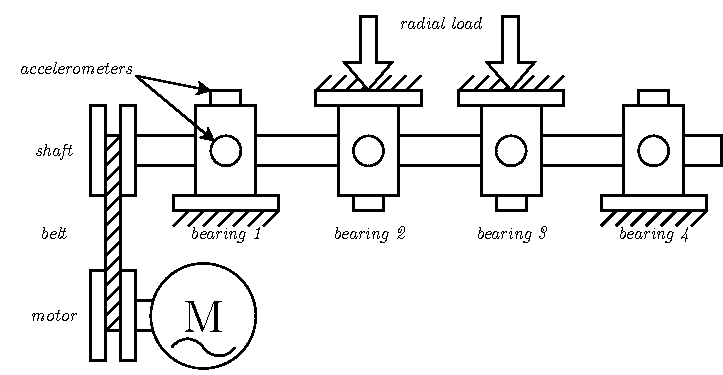
\includegraphics[scale=1]{images/FeatureExtraction/testrig.pdf}
    \caption{The test rig used by \cite{lee2007bearingdataset}}
    \label{fig:IMS_bearing_dataset}
\end{figure}

% \usepackage{tabularray}
\begin{table}
    \centering
    \caption{Test setup \cite{lee2007bearingdataset}}
    \label{tab:IMS_test_parameters}
    \resizebox{\linewidth}{!}{%
    \begin{tblr}{
      cell{2}{1} = {t},
      cell{2}{2} = {t},
      cell{3}{1} = {t},
      cell{3}{2} = {t},
      cell{5}{1} = {t},
      cell{5}{2} = {t},
      cell{6}{1} = {t},
      cell{6}{2} = {t},
      cell{7}{1} = {t},
      cell{7}{2} = {t},
      hline{1,8} = {-}{0.08em},
      hline{2} = {-}{},
    }
     & \textbf{Set No. 1} & \textbf{Set No. 2} & \textbf{Set No. 3}\\
    \textbf{Recording Duration} & 22/10/2003 - 25/11/2003 & 12/02/2004 - 19/02/2004 & 04/03/2004 - 04/04/2004\\
    \textbf{No. of Files} & 2156 & 984 & 4448\\
    \textbf{No. of Channels} & 8 & 4 & 4\\
    \textbf{Channel Arrangement} & {Bearing 1 ch 1  2\\Bearing 2 ch 3  4
    \\Bearing 3 ch 5  6
    \\Bearing 4 ch 7 \& 8~ ~~} & {Bearing 1 ch 1\\Bearing 2 ch 2\\Bearing 3 ch 3\\Bearing 4 ch 4 ~} & {Bearing 1 ch 1\\Bearing 2 ch 2\\Bearing 3 ch 3\\Bearing 4 ch 4~ ~~}\\
    \textbf{File Recording Interval} & 5 or 10 min & 10 min & 10 min\\
    \textbf{Fault type } & {Bearing 3: inner race defect\\Bearing 4: roller element defect} & Bearing 1: outer race failure & Bearing 3: outer race failure
    \end{tblr}
    }
    \end{table}

\section{Time-domain features}
Let's consider a timeserie $\vect{x}$ containing $n$ samples $x_1, x_2, \dots, x_n$. The goal of the feature extraction process is to extract a set of features $\vect{f} = \{f_1, f_2, \dots, f_m\}$ that can be used to describe the signal. In this section, we will describe the features that will be used in the developed framework.
\paragraph{Mean}
The first feature to be considered is simply the mean of the signal. It is defined as
\begin{equation}
    \mu = \frac{1}{n}\sum_{i=1}^n x_i
\end{equation}

\paragraph{\gls{rms}}
The Root mean square of the signal \gls{rms} is related with the power and is defined as
\begin{equation}
    \text{RMS} = \sqrt{\frac{1}{n}\sum_{i=1}^n x_i^2}
\end{equation}

\paragraph{Peack-to-peak}
The peak-to-peak value of the signal is defined as
\begin{equation}
    \text{P2P} = \max(\vect{x}) - \min(\vect{x})
\end{equation}

\paragraph{Standard deviation}
The standard deviation is a measure of the dispersion of the signal and is defined with respect a known distribution with knowledge of the true mean $\mu_{true}$ as

\begin{equation}
    \hat{\sigma} = \sqrt{\frac{1}{n}\sum_{i=1}^n (x_i - \mu_{true})^2}
\end{equation}

but since in our case we don't know the true mean, we will use the sampled standard deviation, that is the best estimate, defined as

\begin{equation}
    \sigma = \sqrt{\frac{1}{n-1}\sum_{i=1}^n (x_i - \mu)^2}
\end{equation}

\paragraph{Skewness}
The skewness is a measure of the asymmetry of the signal and is defined as
\begin{equation}
    \gamma = \frac{1}{n}\sum_{i=1}^n \left(\frac{x_i - \mu}{\sigma}\right)^3
\end{equation}

\paragraph{Kurtosis}
The kurtosis is a measure of the \quoted{peakedness} of the signal and is defined as
\begin{equation}
    \kappa = \frac{1}{n}\sum_{i=1}^n \left(\frac{x_i - \mu_{true}}{\sigma}\right)^4
\end{equation}

and can be estimated on sampled data as

\begin{equation}
  \hat{\kappa} = \frac{(n+1)\,n}{(n-1)\,(n-2)\,(n-3)} \; \frac{\sum_{i=1}^n (x_i - \mu)^4}{k_2^2} - 3\,\frac{(n-1)^2}{(n-2) (n-3)}
\end{equation}}
\mask{\chapter{Proposed Framework}
\label{ch:Framework}}
{\chapter{Embedded implementation}
\label{ch:Embedded}
In \autoref{ch:Framework}, an overview of the framework developed in \texttt{python} was given, relying on the \gls{glo:mongodb} database. This chapter will focus on the implementation of the embedded system. The first big difference is that the embedded system is written in \texttt{C}, which is not an object-oriented language. The second big difference is that the embedded system does not use a database, but it relies only on the variables stored in the RAM. Because of the memory constraints, the training phase relies upon the communication with a \gls{pc} for storing the heavy data. Once the model has been trained, the model is stored in the embedded program and the novelty detection is performed in real time. The general structure is shown in \autoref{fig:Embedded}.

\begin{figure}
    \centering
    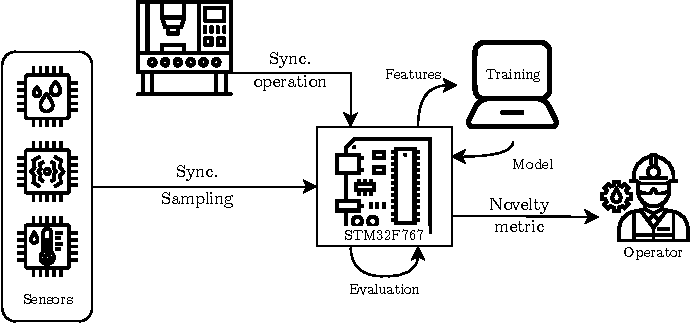
\includegraphics[scale=1]{images/Embedded/EmbeddedStructure.pdf}
    \caption{Embedded system overview}
    \label{fig:Embedded}
\end{figure}


\section{Hardware}
The hardware used for the implementation is the STM32F767ZI board. The characteristics of the board are resumed in \autoref{tab:stm32f767zi}.


\begin{longtable}{p{0.35\linewidth}p{0.55\linewidth}}
    \caption{Hardware characteristics of STM32F767ZI board}    \label{tab:stm32f767zi}\\
    \toprule
    \textbf{Feature} & \textbf{Description} \endfirsthead 
    \hline
    Microcontroller & STM32F767ZI \\
    Architecture & ARM Cortex-M7 \\
    Clock Speed & Up to 216 MHz \\
    Flash Memory & 2 MB \\
    SRAM & 512 KB \\
    EEPROM & No \\
    GPIO & Up to 176 \\
    Timers & 3 x 12-bit, 12 x 16-bit, 2 x 32-bit \\
    ADC & 3 x 12-bit \\
    DAC & 3 x 12-bit \\
    Communication Interfaces & USART, UART, SPI, I2C, CAN, Ethernet, USB \\
    Operating Voltage & 1.7V - 3.6V \\
    Operating Temperature & \SI{-40}{\celsius} to \SI{+150}{\celsius} \\
    \bottomrule    
\end{longtable}

Similarly to what has been done for the \texttt{python} implementation, the parameters of the algorithm are configurable. To avoid the reading of files during the operation, the configuration is held in global variables defined in a header file. The configurable parameters are the usual: depth of the wavelet three, number of features, sampling frequency, time-series length etc.

\section{Software}
The code consists of a main loop, that is continuously running. It is responsible for executing the state machine behaviour, that manages the different phases of operation. The phases of operation are the same as described for the \texttt{python} implementation, except for the training phase, in which the microcontroller performs the sensor polling and the feature extraction and then sends the data to the \gls{pc} using serial communication. The \gls{pc} is responsible for the training phase. This part is developed again in \texttt{python}, but the final model is then formatted as a \texttt{model.h} file that can be directly included in the embedded code. The model is then stored in the flash memory of the microcontroller, together with the rest of the program.

The hardware configuration has been done using the \gls{ide} ({STM32cubeIDE} tool), which is a graphical interface that allows the configuration of the microcontroller and generates the initialization code. 

\subsection{Sensor polling}
The microcontroller comes with a Hardware Abstraction Layer (\gls{hal}) which acts as an intermediary layer between the hardware and software. It simplifies interaction with the microcontroller's peripherals, such as GPIO, UART, and timers, by providing standardized functions and APIs. The \gls{hal} library enhances code reusability across different STM32 microcontroller families, streamlining the development process and enhancing the scalability of embedded systems projects.

To sample the data at a precise sampling frequency, two options are available:
\begin{itemize}
    \item Use the Direct Memory Acces (\gls{dma}) capability of the microcontroller. This approach allows sampling the GPIO and storing the result in the memory accessible by the CPU, without using CPU time. The \gls{dma} is then configured to trigger an interrupt at the end of the transfer, and the interrupt is used to signal the end of the sampling and to start the feature extraction. It is suitable for high sampling frequencies and in fact, even downscaling the clock frequency linked to the \gls{dma} there is a lower bound of obtainable sampling frequencies.
    \item Use the Timer peripheral of the microcontroller. The timer is configured to trigger an interrupt at a precise frequency, and the interrupt causes the CPU to poll the sensor data. This approach is suitable for sampling frequencies that are not too high, and it is the one used in this work (for frequency in the order of \SI{ }{\kilo\hertz}).
    If too many interrupts are generated, the CPU may not be able to execute them instantly, so the actual sampling may shift from the desired frequency, however, in this implementation the only interrupt used is the one for the sampling, so the CPU is not overloaded and the sampling frequency is precise.
\end{itemize}


\subsection{Feature extraction}
The features available to be extracted are the same as the ones described in \autoref{ch:FeatureExtraction}. The time-domain features are coded directly in a function that is responsible for extracting them. The frequency-domain features are computed by another function that relies on the \texttt{C} library \texttt{wavelib} for the wavelet transform \cite{wavelib}. The power of the wavelet coefficients is then computed and appended to the feature vector. The feature vector is then stored in the RAM, and it is used for novelty detection.
The features are then standardized using the same mean and standard deviation used for the training phase. 

\subsection{Evaluation}
When the microcontroller is in the evaluation phase, the feature vector is processed to compute the novelty metric. The model cluster centroids and radiuses were saved in the code in the training phase, so now it is possible to run the \autoref{alg:eval_new_snapshot}. 

\subsection{Custom \texttt{C} functions}
The \texttt{C} main loop, which executes all the behaviours that in the \texttt{python} implementation were executed by the various agents, relies on the library functions as well as on the custom functions resumed in \autoref{tab:custom_functions}.

\begin{longtable}{p{0.4\textwidth}p{0.5\textwidth}}
    \caption{Custom function implemented in \texttt{C}\label{tab:custom_functions}}\\ 
    \toprule
    \textbf{Method} & \textbf{Description} \endfirsthead 
    \hline
    setRTCclock & Set the clock of the microcontroller to the current time \\
    get\_time & Get the current time from the RTC clock \\
    acquireSnapshot & Acquire a snapshot from the sensor \\
    calcSnapDistanceError & Calculate the novelty metric based on the model centroids, radiuses and the current features vector \\
    std\_sclr & Standardize the features vector \\
    snapReadyHandler & Handle the snapshot ready event (the interrupt of the Timer) \\
    norm2 & Compute the norm of a vector \\
    packetCoeff & Perform the Wavelet packed decomposition and compute the norm of the coefficients, it relies on the \emph{wavelib} library \cite{wavelib} \\
    featureExtractor & Extract the features from the snapshot (both time domain and frequency domain) \\
    eucDist & Compute the Euclidean distance between two vectors \\
    \bottomrule
    \end{longtable}}
\mask{\chapter{Validation}
\label{sec:Validation}

This chapter is dedicated to the validation of the framework on real-world data. In \autoref{ch:FeatureExtraction}, the reference dataset \cite{lee2007bearingdataset} has been introduced. Firstly, the \texttt{python} implementation of the framework is validated on the \gls{ims} dataset several times with different configurations to show the flexibility of the framework, and try to find the best configuration for the dataset. 

The first test in the \gls{ims} dataset is carried out with all the machine learning models developed, then only the K-mean model is used in the following tests. In all tests an outlier filter has been implemented, so that the \gls{mla} will warn about the novelty behavior only if two consecutive snapshots are labeled as outliers. 

Then, the \gls{glo:edge} implementation of the framework is validated experimentally on a machine and with a laboratory shaker.



\maskongoig{
\section{\gls{ims} dataset No.1 - Bearing 3x sensor}
\label{sec:ValidationOnRealWorldData}
\begin{figure}
    \centering
    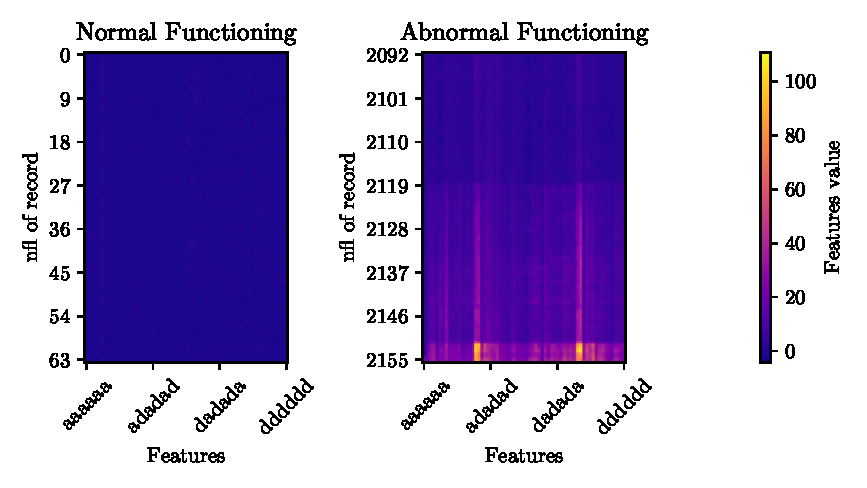
\includegraphics{images/IMS/Heatmap.pdf}
    \caption{Heatmap of the \gls{glo:std} features value for the test $\text{n}^\circ$1 of \gls{ims} dataset}
    \label{fig:Heatmap}
\end{figure}


To start the validation, the test No.1 of the \gls{ims} dataset is subdivided into \emph{training} and \emph{testing} datasets. The first 500 samples are used for training, and the remaining samples are used for testing. 

For all the algorithms, the assumption about the system is that, even if the degradation is continuous, the system is surely healthy until 2003-11-07. The threshold for performing the \gls{nd} is set conformingly to this assumption, for every model considered. Otherwise, the performance of any model could be artificially made as good as desired, by simply setting the threshold to a lower value.

The configuration file is set to use the data from the \quoted{bearing 3x} sensor, extracting all the time-domain and frequency-domain features described in \autoref{ch:FeatureExtraction}. The training dataset is used to train the \gls{mla} to recognize the normal behaviour of the bearing, and the testing dataset is used to validate the trained model. The \autoref{tab:IMS_test_parameters} shows the parameters of test No.1 of the \gls{ims} dataset. For display purposes, the features are \gls{glo:std}, and the heatmap of the \gls{glo:std} features is shown in \autoref{fig:Heatmap} in normal and abnormal conditions.

The abstract version of the \gls{fieldAg} has been used to extract the features from the dataset, creating all the \gls{glo:snap}s in the set $\gls{sym:snapset}=\{\gls{sym:snap}_1,\gls{sym:snap}_2,\dots,\gls{sym:snap}_{500}\}$. These \gls{glo:snap}s are stored in the \emph{unconsumed} collection of the database.

\subsection{Training - K-means}

Using the commands of the \gls{cli}, the training procedure has been launched:
\begin{minted}[linenos,breaklines]{bash}
    C:/Users/JohnSmith/Code/framework> python ./MASTER.py run-feature-agent
    C:/Users/JohnSmith/Code/framework> python ./MASTER.py run-machine-learning-agent novelty train
\end{minted}

where the first command runs the \gls{fieldAg} and the second one runs an \quoted{healthy} instance of the \gls{mla} in training mode.
At this point, the \gls{mla} asks the user to move the \gls{glo:snap}s from the \emph{unconsumed} to the \emph{healthy} collection, since the \emph{healthy} collection is empty. After the confirmation, the \gls{mla} starts the training with a different number of \gls{glo:clust}s and outputs the scoring in the form of silhouette and inertia scores. The results are shown in \autoref{fig:SilScore_01} and \autoref{fig:InertiaScore_01}. The user can confirm that the best number of \gls{glo:clust}s is 2, as the silhouette score is the highest and the inertia score is at the \gls{pof} point, or insert another number of \gls{glo:clust}s, remembering that it is best to overestimate the number of \gls{glo:clust}s to increase the system sensitivity, as discussed in \autoref{sec:wrong_k}. 

In this case, the number of \gls{glo:clust}s has been set to 2, so that the \gls{mla} saves the model trained with $n=2$ into the database. Even if the feature space has high dimensionality, the agent plot to the user also a scatter plot of a subset of features of the training dataset, to have a visual feedback of the \gls{glo:clust}ing, as shown in \autoref{fig:Clusters}, where the points are the \gls{glo:snap}s, the crosses are the centroids and the colours represent the assigned \gls{glo:clust}. We can observe that selecting 2 as the number of \gls{glo:clust}s is adequate and that the projections of the \gls{glo:clust}s' shapes on some planes are not perfectly spherical but, at least, they are not too elongated. This is a good sign for the K-means algorithm, as discussed in \autoref{sec:kmeans_limits}.

\begin{figure}
    \centering
    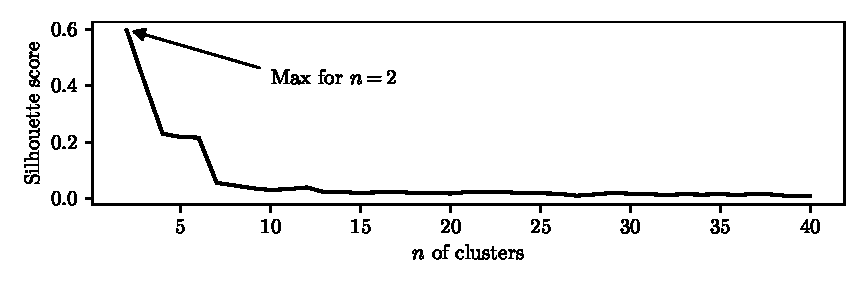
\includegraphics{images/IMS/SilScore_01.pdf}
    \caption{Silhouette score for \gls{glo:clust}ing the test $\text{n}^\circ$1 of \gls{ims} dataset (K-means)}
    \label{fig:SilScore_01}
\end{figure}

\begin{figure}
    \centering
    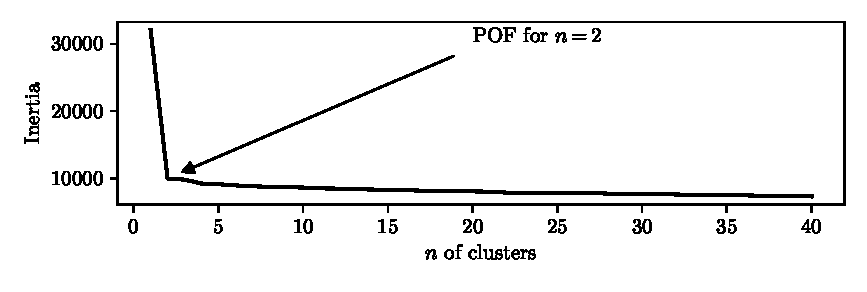
\includegraphics{images/IMS/InertiaScore_01.pdf}
    \caption{Inertia score for \gls{glo:clust}ing the test $\text{n}^\circ$1 of \gls{ims} dataset (K-means)}
    \label{fig:InertiaScore_01}
\end{figure}

\begin{figure}
    \centering
    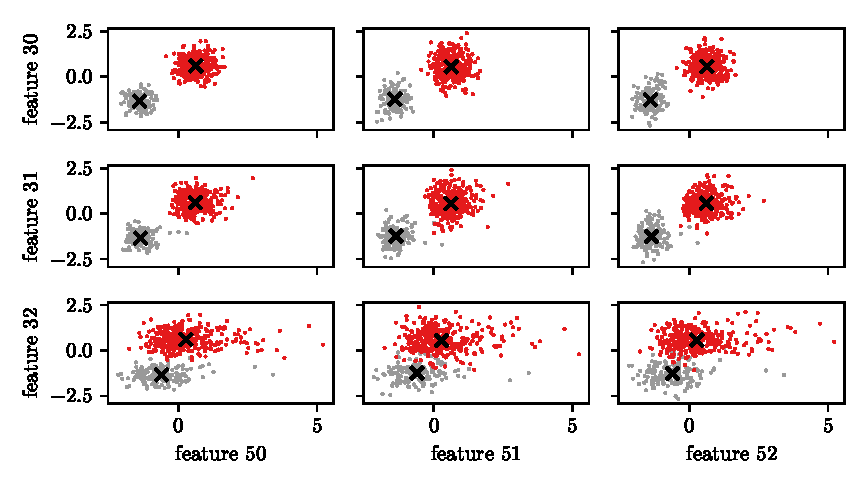
\includegraphics{images/IMS/Clusters.pdf}
    \caption{Scatterplot of training $\gls{glo:snap}$ for the test $\text{n}^\circ$1 of \gls{ims} dataset}
    \label{fig:Clusters}
\end{figure}

\subsection{\gls{nd} Validation - K-means}
Using the validation partition of the dataset, it is possible to set the \gls{mla} in \emph{evaluate} mode. The \gls{fieldAg} uses the validation partition and fills the \emph{raw} collection with the time-series. The {\gls{fa}} extract the features and continuously fill the \emph{unconsumed} collection with the \gls{glo:snap}s. The \gls{mla} evaluates the \gls{glo:snap}s according to \autoref{alg:eval_new_snapshot}  and plots the result, as well as generating a warning if the novelty metric is greater than a certain threshold (in this case 50\%, but it is configurable in the usual \texttt{.yaml} file). The results are shown in \autoref{fig:NoveltyScore_01}, where we can see that the framework detects the novelty quite early, at 2003-11-16 07:46, while the dataset authors, declared the test finished because of bearing defects (not catastrophic failures) at 2003-11-25 23:40. The comparison of the margin of early detection for different algorithms will be resumed later.

In \autoref{fig:NoveltyScore_01_detail}, a detailed view of the \gls{nd} metric becoming consistently greater than the threshold is shown.

\begin{figure}
    \centering
    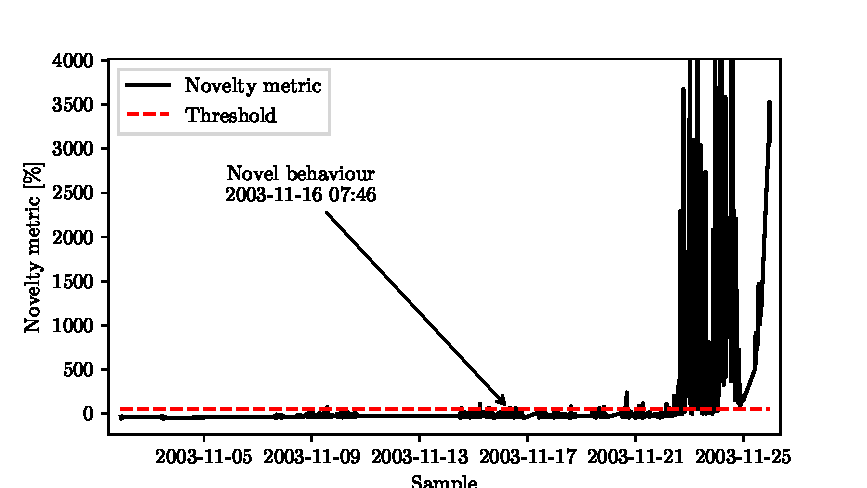
\includegraphics{images/IMS/Novelty_01_500samples_bearing3x.pdf}
    \caption{Results of \gls{nd} for the test $\text{n}^\circ$1 of \gls{ims} dataset (K-means)}
    \label{fig:NoveltyScore_01} 
\end{figure}

\begin{figure}
    \centering
    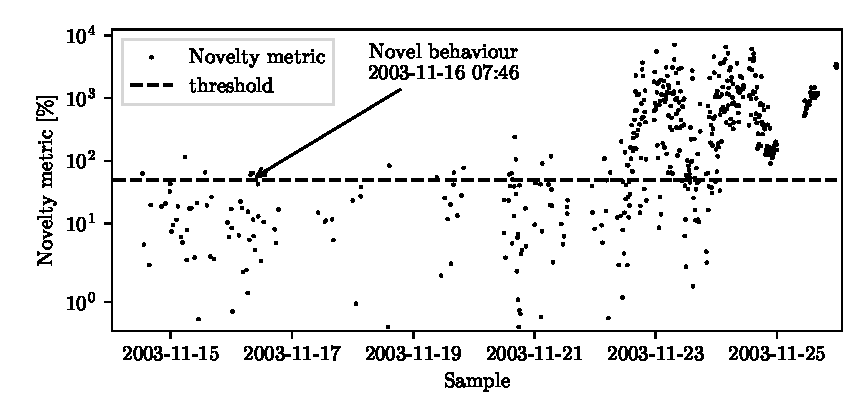
\includegraphics{images/IMS/Novelty_01_500samples_bearing3x_detail.pdf}
    \caption{Results of \gls{nd} for the test $\text{n}^\circ$1 of \gls{ims} dataset (K-means) - detailed view}
    \label{fig:NoveltyScore_01_detail} 
\end{figure}

\subsection{Training - \gls{dbscan}}
Using the same partition of the dataset as for the K-means training, we can train a \gls{dbscan} model. In this case, the silhouette score has to be used to select a suitable value of the radius $\varepsilon$. As shown in \autoref{fig:silscore_dbscan}, the optimal value is 8, which corresponds correctly to the generation of two \gls{glo:clust}s.

\begin{figure}
    \centering
    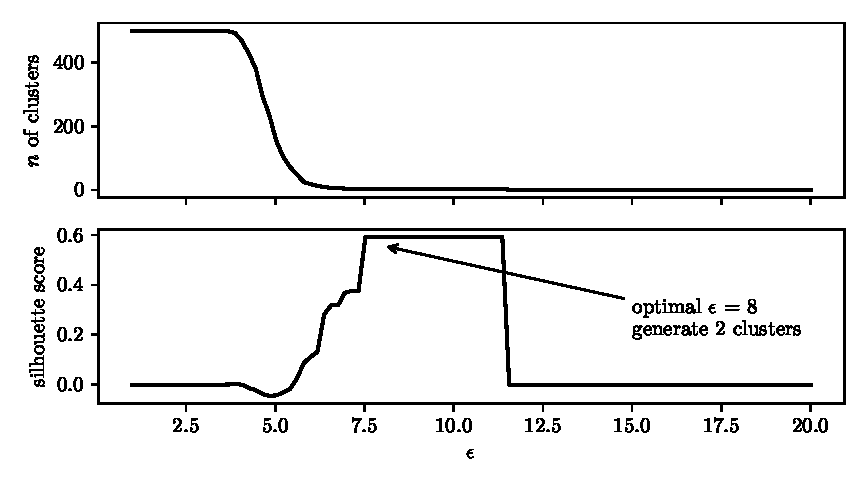
\includegraphics{images/IMS/InertiaScore_01_dbscan.pdf}
    \caption{Silhouette score for \gls{glo:clust}ing the test $\text{n}^\circ$1 of \gls{ims} dataset (\gls{dbscan})}
    \label{fig:silscore_dbscan}
\end{figure}

\subsection{\gls{nd} Validation - \gls{dbscan}}
As it has been done for the K-means, the validation partition of the dataset is now used for performing \gls{nd} with the \gls{dbscan} model, as described in \autoref{sec:dbscan_eval}. The result is shown in \autoref{fig:NoveltyScore_01_dbscan}, where we can see that the \gls{dbscan} model detects the novelty at 2003-11-22 15:06, that is quite early, but not as early as the K-means model. This is because the metric generated by the \gls{dbscan} model has a greater variance so, instead of increasing consistently, it overshoots the threshold quite before this time but fails to consistently stay above the threshold. 

\begin{figure}
    \centering
    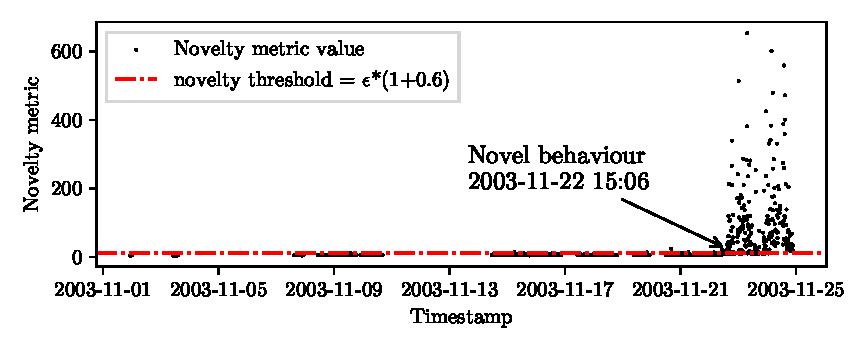
\includegraphics{images/IMS/Novelty_01_500samples_bearing3x_dbscan.pdf}
    \caption{Results of \gls{nd} for the test $\text{n}^\circ$1 of \gls{ims} dataset (\gls{dbscan})}
    \label{fig:NoveltyScore_01_dbscan}
\end{figure}

\subsection{Training - \gls{gmm}}
Let's now try with the \gls{gmm} model. The metric for selecting the number of \gls{glo:clust}s is now the \gls{bic} and the \gls{aic}, as shown in \autoref{fig:bic_aic_gmm}. The two metrics diverge but, as discussed in \autoref{sec:gauss_train}, the \gls{aic} tends to perform better. In this case, minimizing the \gls{aic} leads to select 25 as the number of \gls{glo:clust}s, which is much more than what was selected with the K-means, but still a reasonable choice, also considering that the \gls{gmm} is a soft \gls{glo:clust}ing algorithm and that we are using the density as a metric to perform \gls{nd}.

\begin{figure}
    \centering
    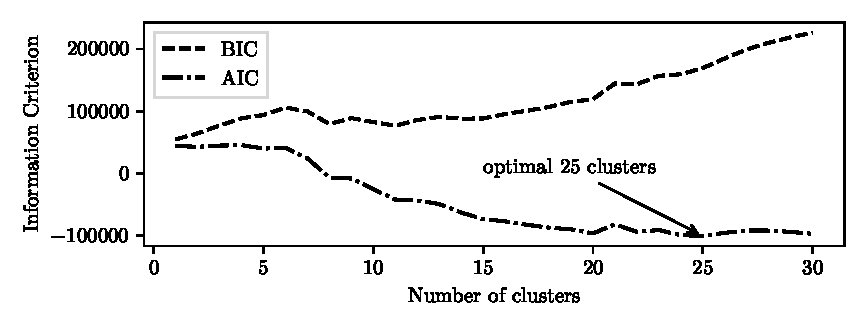
\includegraphics{images/IMS/BICAIC_GMM.pdf}
    \caption{\gls{bic} and \gls{aic} for \gls{glo:clust}ing the test $\text{n}^\circ$1 of \gls{ims} dataset (\gls{gmm})}
    \label{fig:bic_aic_gmm}
\end{figure}

\subsection{\gls{nd} Validation - \gls{gmm}}
The validation partition of the dataset is now used for performing \gls{nd} with the \gls{gmm} model. The result is shown in \autoref{fig:NoveltyScore_01_gmm}, where we can see that the \gls{gmm} model detects the novelty at 2003-11-22 03:47. The considerations about this result are the same as for the \gls{dbscan} model, and in fact, the timestamp of the detection event is really close to the one obtained with \gls{dbscan}. In \autoref{fig:NoveltyScore_01_gmm}, the metric (density value) appears in coloured dots, as each colour represents the \gls{glo:clust} to which the \gls{glo:snap} has been assigned.
\begin{figure}
    \centering
    \includegraphics{images/IMS/Novelty_01_500samples_bearing3x_gmm.pdf}
    \caption{Results of \gls{nd} for the test $\text{n}^\circ$1 of \gls{ims} dataset (\gls{gmm})}
    \label{fig:NoveltyScore_01_gmm}
\end{figure}

\subsection{\gls{nd} Validation - Bayesian \gls{gmm}}
The other Gaussian model is the \gls{bgmm}, since this approach is totally unsupervised, only the validation results are reported here. The result is shown in \autoref{fig:NoveltyScore_01_bgmm}, where we can see that the \gls{bgmm} model detects the novelty around the same time as the \gls{gmm} model, at 2003-11-22 03:45.

In both \gls{gmm} and \gls{bgmm} the metric (density value) spans a lot of decades, so the plots are done on a logarithmic scale.

\begin{figure}
    \centering
    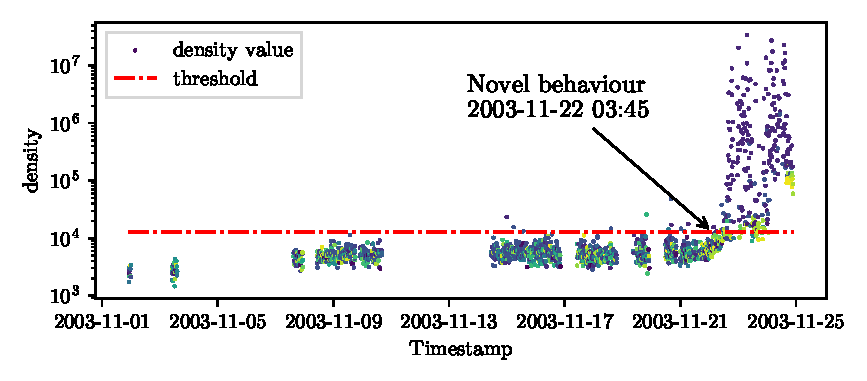
\includegraphics{images/IMS/Novelty_01_500samples_bearing3x_GMM_bayesan.pdf}
    \caption{Results of \gls{nd} for the test $\text{n}^\circ$1 of \gls{ims} dataset (\gls{bgmm})}
    \label{fig:NoveltyScore_01_bgmm}
\end{figure}

\subsection{\gls{nd} Validation - \gls{nu_svm}}
The next algorithm to test is the \gls{nu_svm}. Again, this is totally unsupervised, so only the validation results are reported here. The novelty metric evolution over time is shown in \autoref{fig:NoveltyScore_01_nusvm}, where we can see that the \gls{nu_svm} model detects the novelty at 2003-11-22 14:56, which is comparable with the \gls{dbscan} and \gls{gmm} models.

\begin{figure}
    \centering
    \includegraphics{images/IMS/Novelty_01_500samples_bearing3x_nusvm.pdf}
    \caption{Results of \gls{nd} for the test $\text{n}^\circ$1 of \gls{ims} dataset (\gls{nu_svm})}
    \label{fig:NoveltyScore_01_nusvm}
\end{figure}

\subsection{\gls{nd} Validation - \gls{iforest}}
The second last technique to test is the one based on the \gls{iforest} model. The result is shown in \autoref{fig:NoveltyScore_01_iforest}, where we can see that the \gls{iforest} model detects the novelty at 2003-11-16 10:08:46, which is a good result comparable with the K-means model. The problem with the metric of the \gls{iforest} is that it increases a lot the variance around the \gls{nd} event, but the mean does not increase consistently, so a lot of \gls{glo:snap}s are discarded as outliers, before the \gls{nd} event. 

This is, in my opinion, a promising approach. With these settings a lot of \gls{glo:snap}s are discarded as outliers, but with a different outlier filter, based on the percentage of novelty samples in a window, the \gls{iforest} model could perform even better.
\begin{figure}
    \centering
    \includegraphics{images/IMS/Novelty_01_500samples_bearing3x_iforest.pdf}
    \caption{Results of \gls{nd} for the test $\text{n}^\circ$1 of \gls{ims} dataset (\gls{iforest})}
    \label{fig:NoveltyScore_01_iforest}
\end{figure}

\subsection{\gls{nd} Validation - \gls{lof}}
The last algorithm to test is the \gls{lof}. The result is shown in \autoref{fig:NoveltyScore_01_lof}, where we can see that the \gls{lof} model detects the novelty at 2003-11-16 07:49, which is a good result comparable with the K-means model. It doesn't have the same problem as the \gls{iforest}, as there aren't as many discarded \gls{glo:snap}s before the \gls{nd} event.

\begin{figure}
    \centering
    \includegraphics{images/IMS/Novelty_01_500samples_bearing3x_lof.pdf}
    \caption{Results of \gls{nd} for the test $\text{n}^\circ$1 of \gls{ims} dataset (\gls{lof})}
    \label{fig:NoveltyScore_01_lof}
\end{figure}

\subsection{Comparison of the results}

\subsubsection{Comparison between the models}

\begin{table}
    \centering
    \caption{Comparison of the results for the test $\text{n}^\circ$1 of \gls{ims} dataset.}
    \label{tab:ims01_comparision}
    \begin{tabular}{lrr} 
    \toprule
    \textbf{Algorithm} & \textbf{\gls{nd} event} & \textbf{\gls{glo:leadtime} }{[}min] \\ 
    \hline
    K-means & 2003-11-16 07:46 & \textbf{13913} \\
    \gls{dbscan} & 2003-11-22 15:06 & 4833 \\
    \gls{gmm} & 2003-11-22 03:47 & 5513 \\
    \gls{bgmm} & 2003-11-22 03:45 & 5514 \\
    \gls{nu_svm} & 2003-11-22 14:56 & 4844 \\
    \gls{iforest} & 2003-11-16 10:08 & 13771 \\
    \gls{lof} & 2003-11-16 07:48 & 13912 \\
    {P2P} without any \gls{ml} & 2003-11-22 16:06 & 4774 \\
    \bottomrule
    \end{tabular}
\end{table}

In \autoref{tab:ims01_comparision}, the results of all the previous tests are resumed, together with the result of performing \gls{nd} without any machine learning algorithm, but just setting a threshold on the P2P value of the time-series, as it was previously shown in \autoref{fig:IMS_TD_features}. This last basic approach detects the novelty around the afternoon of 2003-11-22. 

The \gls{nu_svm} and the \gls{dbscan} models are not performing much better than not even using machine learning (at least on this dataset signal). The \gls{gmm} and \gls{bgmm} models are performing slightly better, but the margin is so low that the result may be biased by the threshold setting. The \gls{iforest}, \gls{lof} and K-means models are performing better, they are all very close to detecting the novelty, around 14000 min = 9.7 days before the end of the test. The K-means model is the one performing the best, but just slightly better than the \gls{iforest} and \gls{lof} models so, again, this small difference may not be significant. However, as discussed in the previous chapters, the K-means model will be used in the rest of the work, as it is also the most simple and interpretable model.


\subsubsection{Comparison with another approach}
As anticipated in the \autoref{ch:state_of_the_art}, about the State of the Art, the signal of the same bearing (Bearing 3x) of this same test has been used in \cite{Umberto}. In their research, the authors used a different approach, based on regression, and obtained the result reported in \autoref{fig:umbertoresult}


\subsubsection{Comment about the comparison}
Every system that outputs a warning based on a trigger on a threshold is highly sensitive to the value of the threshold itself. This means that the comparison of the results is not straightforward, and quite opinable, because selecting a low threshold will make almost every system trigger earlier. The measure to take into consideration, in my opinion, is how many false positives are generated if the threshold is lowered, and how small the variance of the metric is. A high variance, on this dataset, means that the system is very sensitive while evaluating quite similar signals.

\subsection{\gls{rul} Predictions validation - K-means}
After the \gls{nd} event, the \gls{mla} starts predicting the future evolution of the novelty metric, and it superimposes the prediction curve to the same plot displayed to the user. The fitting procedure is the closed form solution of the \gls{ls} problem applied to an exponential curve of \autoref{eq:exp_degradation_2}, as described in \autoref{sec:predictions}. The samples used for the regression of the curve are the last 230 before the current one. This parameter of the framework is configurable in the \texttt{.yaml} file. 

Some good predictions are shown in \autoref{fig:RULPredictions01}. The \gls{rul} is the difference between the intercept of the prediction curve and another threshold, higher than the one used for \gls{nd}, and the current time. In the figure, the blue line is a prediction made just a few hours after the \gls{nd} event (the vertical dashed line marks the time of the prediction). The same concept applies to the other predictions performed in later times.

In some circumstances, the novelty metric starts decreasing slightly, on average, as can be seen around 2003-11-21. In this case, if the novelty metric has this behaviour for several \gls{glo:snap}s ($\approx 230$), the fitted curve will be a decreasing exponential, as shown in \autoref{fig:RULPredictions01_fail}. 

If this situation occurs, the intercept with the threshold does not exist, and the \gls{rul} prediction fails, so the interpretation of the \gls{rul} is left to the user. In some cases, the defect in a system can \quoted{self-heal} (for example a crack in a bearing can be polished with the use \cite{IMSpaper}). If this behaviour is possible for the system, this situation can be interpreted as a sign that the system is going to return to normality. Otherwise, the user can retain the previous \gls{rul} prediction as the \gls{rul} of the system.

\begin{figure}
    \includegraphics{images/IMS/Novelty_01_500samples_bearing3x_predictions.pdf}
    \caption{\gls{rul} prediction at different instants after the \gls{nd} event (dashed lines are the instants of the predictions corresponding to the same-colour solid line prediction)}
    \label{fig:RULPredictions01}
\end{figure}

\begin{figure}
    \includegraphics{images/IMS/Novelty_01_500samples_bearing3x_predictions_failed.pdf}
    \caption{Failed \gls{rul} prediction.}
    \label{fig:RULPredictions01_fail}
\end{figure}

\subsection{Retraining,  evaluating and predicting after \gls{nd} event}
If the user, after the \gls{nd} event, performs an investigation that leads to the belief that the system is still healthy, the user can turn the \gls{mla} in \emph{retrain} mode. In this case, the \gls{glo:snap}s that are in the quarantine collection, are moved to the healthy collection (faulty if the instance is for \gls{fd} and the investigation reveals that the fault is real). 
The model is then retrained with the new data with the same procedure used for the first training (silhouette and inertia scores are computed and the user is asked to confirm the number of \gls{glo:clust}s).

Let's investigate what would have happened if the user declared the system healthy at 2003-11-23 00:00, in the previous scenario of  \quoted{Bearing 3 x} signal in the \gls{ims} dataset. The \gls{mla} suggests that the best number of \gls{glo:clust}s is still two, so it has been retrained with the new data. The result of the updated model performing \gls{nd} is shown in \autoref{fig:NoveltyScore_01_retrained}. The predictions of the \gls{rul} are shown in \autoref{fig:RULPredictions01_retrained}. 

This test shows that in an increasingly decaying system retrained with data very close to the fault condition the \gls{mla} is able to detect the fault again. This comes at the cost of a later detection, and the first predictions after the \gls{nd} event are not as good as the previous ones. Anyway, the \gls{rul} predictions still become more accurate as time passes, and the \gls{rul} prediction at the end of the test is still quite accurate (on the same day of the event). 

Another consideration is about the \gls{rul} threshold: since the model has been retrained with \quoted{worse} data, the threshold for the \gls{rul} prediction should be set to a lower value, because now the \gls{glo:clust}s are either more in quantity, distorted or bigger, so it is unlikely that the novelty metric can still reach the same high values estimated before the retraining.

An intuition about why the sensitivity of the system is reduced after the retraining comes by examining the scatter plot of the \gls{glo:snap}s in the feature space, shown in \autoref{fig:Clusters_novelty}, where all the \gls{glo:snap}s extracted from the dataset are displayed. The \gls{glo:clust}s are more elongated and much bigger. These shapes arise gradually from the original ones of \autoref{fig:Clusters} so, by performing a retrain, both the effect of producing bigger \gls{glo:clust}s and one of the \gls{glo:clust}s being much more elongated play a role in reducing the sensitivity of the \gls{mla}.

\begin{figure}
    \centering
    \includegraphics{images/IMS/Novelty_01_500samples_bearing3x_retrained.pdf}
    \caption{Results of \gls{nd} for the test $\text{n}^\circ$1 of \gls{ims} dataset (K-means) - retrained model}
    \label{fig:NoveltyScore_01_retrained}
\end{figure}

\begin{figure}
    \centering
    \includegraphics{images/IMS/Novelty_01_500samples_bearing3x_predictions_retrained.pdf}
    \caption{\gls{rul} prediction at different instants after the \gls{nd} event with the retrained model (dashed lines are the instants of the predictions corresponding to the same-colour solid line prediction)}
    \label{fig:RULPredictions01_retrained}
\end{figure}

\begin{figure}
    \centering
    \includegraphics{images/IMS/Clusters_novelty.pdf}
    \caption{Scatterplot of all the $\gls{glo:snap}$ for the test $\text{n}^\circ$1 of \gls{ims} dataset}
    \label{fig:Clusters_novelty}
\end{figure}


\section{Experiments on a laboratory shaker - Test 1}
\label{sec:shaker_test01}

After the \gls{pc} implementation of the \gls{glo:frmwrk} has been tested widely on the \gls{ims} dataset, the \gls{glo:edge} implementation had to be validated experimentally. The first test was done with a laboratory shaker, which is basically a powerful active speaker with a really wide band that can be attached with a bolt to a structure, to vibrate it.

In this case, an accelerometer, whose key specifications are shown in \autoref{tab:adxl335_specifications}, was used to capture the vibration signal. The accelerometer was attached to the shaker, with a custom 3D-printed fixture. This first test has the scope of checking the capability of the \gls{glo:edge} implementation to detect a new low amplitude harmonic in the signal. The signal is generated as a \texttt{.wav} file and fed to the shaker by a player. Both the input of the shaker and the output of the accelerometer were monitored with a digital oscilloscope. The setup is shown in \autoref{fig:shaker_setup}.



\begin{table}[h]
    \centering
    \caption{Specifications of the ADXL335 Accelerometer}
    \label{tab:adxl335_specifications}
    \begin{tabular}{ll} 
    \toprule
    \textbf{Parameter} & \textbf{Value} \\ 
    \hline
    Supply Voltage & 1.8V to 3.6V \\
    Sensing Range & ±3g \\
    Sensitivity & 300 mV/g \\
    Bandwidth & 0.5 Hz to 1600 Hz \\
    Output Type & Analog \\
    Output Voltage Range & 0V to V$_{CC}$ \\
    Operating Temperature & -40°C to +85°C \\
    Package & $3\si{mm} \times 5 \si{mm} \times 1 \si{mm}$ \\
    \bottomrule
    \end{tabular}
\end{table}

\begin{figure}
    \centering
    \includegraphics[width=.4\textwidth]{Images/shaker/IMG_20231207_103126143.jpg}
    \caption{Setup of the shaker tests.}
    \label{fig:shaker_setup}
\end{figure}
\begin{table}
    \centering
    \caption{Harmonic coefficients for the shaker test. Wave 1 and Wave 2 are training signals, and Harmonic Injection is the signal to be detected.}
    \label{tab:shaker_param_01}
    \begin{tabular}{lccccccc} 
    \toprule
    \multirow{2}{*}{\textbf{Signal Name }} & \multicolumn{6}{c}{\textbf{Harmonic frequency} [Hz]} & \multirow{2}{*}{\textbf{Amplitude} [mV]$_{pp}$} \\
     & 30 & 70 & 100 & 300 & 800 & 1400 &  \\ 
    \hline
    Wave 1 & 0.1 & 1.0 & 1.0 & \multicolumn{1}{c}{-} & 1.0 & 1.0 & 1000 \\
    Wave 2 & 0.1 & 0.8 & 1.0 & \multicolumn{1}{c}{-} & 3.0 & 0.6 & 1000 \\
    Harmonic Injection & 0.1 & 1.0 & 1.0 & 0.1 & 1.0 & 1.0 & 1000 \\
    \bottomrule
    \end{tabular}
    \end{table}

\subsection{Training and evaluating}
The \gls{glo:frmwrk} was firstly set to gather the data, extract the \gls{glo:feature}s according to the configuration, and send the data to the \gls{pc} for training. The training signals are two waves with different harmonic content and the test signal is very similar to one used for training, except for the presence of an additional harmonic with a small amplitude. The train and test signals harmonic content is reported in \autoref{tab:shaker_param_01}. The amplitude of the vibration has been tuned at each test to ensure that the microcontroller was reading a signal of 1V$_{pp}$. The amplitude of the signals has been kept constant to test the capability of the \gls{glo:frmwrk} to detect the frequency content of the signal in the \gls{glo:feature} extraction phase. The waveform of the test signals is shown with the one of one training signal in \autoref{fig:shaker}, to show the similarity of the two signals. 

The setting of the \gls{glo:frmwrk} can be resumed as follows:
\begin{itemize}
    \item 67 \gls{glo:feature}s extracted from the signal ($2^6=64$ \gls{glo:feature}s from the wavelet decomposition, mean, P2P, and \gls{rms});
    \item 110 samples for training for each signal.
    \item sampling frequency of 5kHz, for 1s of acquisition.
\end{itemize}

After the data gathering was completed, the training was done on the \gls{pc}, as usual. The silhouette score correctly suggested 2 as the best number of \gls{glo:clust}s to be used. The \gls{pc} part of the \gls{glo:frmwrk} outputs the \texttt{model.h} file directly in the embedded project folder, so just a new upload of the firmware was needed to test the detection. The microcontroller was then set in \emph{evaluation} mode and both the two training signals and the test signal were fed to the shaker. 

\subsection{Results}
The result of the novelty detection is shown in \autoref{fig:shaker_results}. The result is consistent with the expected outcome, as the training signals produced a negative novelty metric, while the test signal produced a positive (and quite high) novelty metric. The spectrum of the signals used is shown graphically in \autoref{fig:shaker_spectrum}.

\begin{figure}
    \centering
    \includegraphics{Images/shaker/Figure_1.pdf}
    \caption{Waveform comparison of the shaker test.}
    \label{fig:shaker}
\end{figure}

\begin{figure}
    \centering
    \includegraphics{Images/shaker/Results.pdf}
    \caption{Novelty detection result}
    \label{fig:shaker_results}
\end{figure}

\begin{figure}
    \centering
    \includegraphics{Images/shaker/spectrum.pdf}
    \caption{Spectrum of the waveforms.}
    \label{fig:shaker_spectrum}
\end{figure}



\section{Experiments on a laboratory shaker - Test 2}
\label{sec:shaker_test02}
In the previous section, the first test on the shaker was presented. The test has shown the capability of the framework to detect unknown harmonics. A second test was done to evaluate the capability to detect time-domain variations and the effect of reducing the frequency resolution. 

\subsection{Training and evaluating}
This new configuration has been set to use only 4 frequency-domain features and the same 3 time-domain features of the previous test, for a total of 7 features. The signal used for training and testing is resumed in \autoref{tab:shaker_param_02}. The set is composed of the same signal at different amplitudes used for training and testing, plus another signal with different frequency content but the same amplitude as a training signal used for testing. 

The training has been carried out in the same way as the previous test, the training of the K-means model has been done with 4 \gls{glo:clust}s, and loaded on the microcontroller. 

\begin{table}
    \centering
    \caption{Parameters of the second shaker test.}
    \label{tab:shaker_param_02}
    \begin{tabular}{cccccccc} 
    \toprule
    \multicolumn{5}{c}{\textbf{Harmonic frequency} {[}Hz]} & \multirow{2}{*}{\textbf{Amplitude }{[}mV$_{pp}$]} & \multicolumn{2}{c}{\textbf{ No. of \gls{glo:snap}s}} \\
    10 & 30 & 60 & 70 & 100 &  & Train & Test \\ 
    \hline
    - & 0.1 & - & 1.0 & 1.0 & 580 & 100 & 10 \\
    - & 0.1 & - & 1.0 & 1.0 & 1000 & 100 & 10 \\
    - & 0.1 & - & 1.0 & 1.0 & 1980 & 100 & 10 \\
    - & 0.1 & - & 1.0 & 1.0 & 1540 & 100 & 10 \\
    - & 0.1 & - & 1.0 & 1.0 & 2000 & - & 20 \\
    - & 0.1 & - & 1.0 & 1.0 & 0 & - & 10 \\
    - & 0.1 & - & 1.0 & 1.0 & 800 & - & 10 \\
    - & 0.1 & - & 1.0 & 1.0 & 200 & - & 10 \\
    - & 0.1 & - & 1.0 & 1.0 & 1220 & - & 10 \\
    1.0 & 1.0 & 0.1 & - & - & 1540 & - & 10 \\
    \bottomrule
    \end{tabular}
    \end{table}



\subsection{Results}
\begin{figure}
    \centering
    \includegraphics{Images/shaker/Test02.pdf}
    \caption{Novelty detection result}
    \label{fig:shaker_results02}
\end{figure}
The result of the novelty detection is shown in \autoref{fig:shaker_results02}. The first 4 lines have been correctly identified as normal, as they were in fact a repetition of the training signals.
Then the purple and cyan line in the figure is the same training signal, but 20 mV higher in amplitude \gls{wrt} the training signal. The novelty metric overshoots the threshold in 5 samples out of 20. An increase of 2\% in amplitude generates the \gls{nd} event 25\% of the times can be observed with this signal. 

The brown, grey and light-green lines are the same signal, but with a bigger difference in amplitude \gls{wrt} the training signal. All the \gls{glo:snap}s of these signals correctly generated a novelty metric above the threshold. The blue line is the signal with a different frequency content, and it has been correctly identified as a novelty event, this is the confirmation that even with just 4 frequency bins, the wavelet decomposition is still generating features that are informative.

The pink line is the test signal with an amplitude of 800mV. It's evident that the novelty metric is below the threshold, and the signal has been classified as normal even if it is not in the training dataset. Let's investigate how this happened. The first consideration is that the 800mV amplitude is quite tight to both the 1000mV and 580mV signals used for training. Moreover, in this case, the total number of features is just 7. This allows plotting all the features against each other, to see why the \gls{nd} event has not been detected. In \autoref{fig:shaker_conf_matrix} the scatter plot of the features is shown. It's evident that, in this environment, even performing the standardization of the features, the \gls{glo:clust}s are still very elongated, resembling almost a line. To fit an elongated \gls{glo:clust} in a hypersphere, it is inevitable that in some sections, the hypersphere will not closely surround the \gls{glo:clust}, leaving \quoted{space} for false negative results. Another problem is that the k-means algorithm tends to split long \gls{glo:clust}s. In the figure, the red dots are the false negative results, and the grey shades are the hypersphere projection on the considered features plane. The black dots are the training data. The effect of the elongated \gls{glo:clust}s is particularly evident in the plot of the \quoted{Feature 3} against \quoted{Feature 2}, where the red dots are in between two \gls{glo:clust}s, that are modelled as one. On the other hand, looking at the plot of \quoted{Feature 1} against \quoted{Feature 4}, a very long \gls{glo:clust} has been split in two. This is an example of exploiting the limitations of the k-means algorithm anticipated in \autoref{sec:kmeans_limits}. 
For completness, in \autoref{fig:shaker_conf_matrix}, also the true positive results are shown, as magenta dots.


\begin{figure}
    \centering
    \includegraphics{Images/shaker/ConfusionMatrix.pdf}
    \caption{False Negative and True Positive results. On the diagonal, there is a histogram of the feature values. The off-diagonal plots are the scatter plots of the features. The shades are the projection of the \gls{glo:clust}s on the considered plane. (Red: False Negative, Magenta: True Positive, Black: training data)}
    \label{fig:shaker_conf_matrix}
\end{figure}
\clearpage

\subsection{Possible improvements}
The environment of this test is very challenging for the k-means algorithm. As discussed in \autoref{ch:Unsupervised}, there are algorithms that are not affected by the \gls{glo:clust}s' shapes. The candidate algorithms that may perform better in this situation are the \gls{lof}, the \gls{iforest} and \gls{dbscan}. Future work could be to implement these algorithms in the \gls{glo:edge} framework, despite being more demanding in computational power and memory, and test them in this environment.

As proof of concept, the \gls{lof} implementation in \texttt{\gls{glo:python}} has been used to perform \gls{nd} on the same dataset used in this section in \gls{glo:edge}. The results are reported in \autoref{label:lof_results}. The \gls{lof} algorithm has been able to correctly identify all the \gls{nd} events, even the signals with just 20mV variation from the training dataset, and the 800mV signal that was problematic for the K-means. The \gls{lof}, however, generated a false positive on the 580mV signal. This false positive may be avoided by increasing the threshold, but this would also increase the false negative rate. 

\begin{figure}
    \centering
    \includegraphics{Images/shaker/Test02_LOF.pdf}
    \caption{\gls{lof} novelty detection result}
    \label{fig:lof_results}
\end{figure}
\section{Experimental validation}
\label{sec:ExperimentalValidation}
}}
\mask{\chapter{Conclusion and future work}
\label{ch:Conclusion}

The proposed \gls{glo:frmwrk} has demonstrated the capability of detecting anomalies in generic time domain data. The proposed modular structure is a key for enabling the \gls{glo:frmwrk} to be considered a prototype that can be applied to a wide range of applications. The unsupervised learning approach further eases and accelerates the adaptation of this solution into different domains. 

The deployment of the solution also for \gls{glo:edge} enables the \gls{glo:frmwrk} to expand the range of applicability beyond classical industrial environments, toward non-standard applications. The intrinsic cybersecurity of edge devices is a nice byproduct that can be exploited whenever the \gls{glo:frmwrk} is deployed in a critical infrastructure.

In future work, there is significant potential for further testing and refinement of the already developed \gls{glo:frmwrk}. One path to explore involves testing the edge implementation on a degrading system rather than relying on simulated degradation through environmental parameter changes. This approach could provide invaluable insights into the robustness and adaptability of the \gls{glo:frmwrk} in critical scenarios. Additionally, deploying the remaining algorithms within the edge \gls{glo:frmwrk} to address the limitations of K-means \gls{glo:clust}ing presents an exciting opportunity. Since the repertoire of algorithms shown promising results on real word datasets, deploying all of them also in the edge version of the \gls{glo:frmwrk} allows to offer a more comprehensive solution to complex problems in \gls{glo:edge} environments.

The \gls{glo:frmwrk} could also be enhanced from the user experience perspective by developing a Graphical User Interface (\gls{gui}) that allows to interact with the \gls{glo:frmwrk} in a more intuitive way. The already developed \gls{cli} could remain a secondary option for advanced users, or be used in the background by the \gls{gui} to execute the \gls{glo:frmwrk}'s functionalities. }



% \paginavuota % it works even without stile=classica

\appendix
% appendix
\mask{\chapter{Fourier Transform}
\label{app:FFT}
This appendix aims to provide a brief and non-exhaustive introduction to the Fourier Transform. The various types of Fourier Transform are key tools in a vast range of fields in engineering, physics and mathematics. In computer science, the Fourier Transform is used in signal processing, image processing, data compression, and many other applications.

\section{Continuous Fourier Transform}
\label{sec:ContinuousFourierTransform}
Most of the modern signal processing techniques find their roots in the Fourier Transform, which is a mathematical tool that allows the decomposition of a non-periodic signal into its frequency components. For periodic signals, The transform is a train of impulses, whose amplitudes are linked to the Fourier series coefficients.

The Continuous Fourier Transform (\gls{cft}) of a signal $x(t)$ is defined as:
$$
X(f) = \int_{-\infty}^{\infty} x(t) e^{-j2\pi ft} dt, \qquad \forall f \in \mathbb{R}
$$
where $X(f)$ is the Fourier Transform of $x(t)$, $f$ is the frequency variable and $j$ is the imaginary unit. The quantity $2\pi f$ is the angular frequency.

\section{Discrete Fourier Transform}
\label{sec:DiscreteFourierTransform}
The Discrete Fourier Transform (\gls{dft}) is a sampled version of the Continuous Fourier Transform. 
From an engineering perspective, the DFT is of particular interest because most of the signals are sampled in time and therefore, the \gls{dft} is the most commonly used form of the Fourier Transform.

The \gls{dft} is used to transform a sequence of $N$ complex numbers $x(n)$ into another sequence of $N$ complex numbers $X(k)$. The DFT is defined as:
\begin{equation}
\label{eq:DFT}
X(k) = \sum_{n=0}^{N-1} x(n) e^{-j2\pi kn/N}, \qquad \forall k \in \{0, 1, \ldots, N-1\}
\end{equation}
where $X(k)$ is the \gls{dft} of $x(n)$, $k$ is the frequency index and $N$ is the number of samples in the sequence.

The output spectrum given by the \gls{dft} is also discrete and finite, with the same number of samples as the input signal. 
The sampling frequency of the signal $x(n)$ determines the upper frequency limit of the \gls{dft} output, as the faster the sampling rate, the higher the frequencies that can be represented. The length of the signal $x(n)$ determines the frequency resolution of the \gls{dft} output, as the longer the signal, the finer the frequency resolution is.

\paragraph{Computational complexity}
Examining the definition of the \gls{dft} in Equation \ref{eq:DFT}, we can notice that it requires $N$ complex multiplications and $N(N)$ complex additions. Therefore, the computational complexity of the \gls{dft} is $\mathcal{O}(N^2)$, which does not scale well for large values of $N$.

\section{Fast Fourier Transform}
\label{sec:FastFourierTransform}

To overcome the computational complexity of the \gls{dft}, the Fast Fourier Transform (\gls{fft}) algorithm was developed in the 1960s by Cooley and Tukey \cite{cooley1965algorithm}. Choosing a data length $N$ that is a power of 2, the \gls{fft} algorithm reduces the computational complexity of the \gls{dft} from $\mathcal{O}(N^2)$ to $\mathcal{O}(N \log_2 N)$. This becomes particularly important for large values of $N$, where the \gls{fft} algorithm is significantly faster than the \gls{dft}.

In the classic algorithm, a single multiplication happens many times. The general idea of this fast algorithm is to exploit the periodicity of the complex exponentials in the \gls{dft} to divide the computation into smaller sub-problems and reuse the already computed multiplication. 

Breaking the exponential into its sine and cosine components, it becomes intuitive that the same result appears multiple times in the computation. The \gls{fft} algorithm takes advantage of this redundancy to reduce the number of operations, recursively dividing the problem into half-sized subproblems up to the point that the subproblems have only one sample.
}
\mask{\chapter{Wavelet Transform}
\label{app:wavelet}}


% endnotes here if needed

\customClearDoublePage
\printbibliography[heading=bibintoc] % heading required to show it in ToC

\end{document}
